%\section{Reproducibility Appendix}
\section{Supplementary Information}
\label{sxn:appendix}


\subsection{Supplementary Tables} 

\paragraph{Reproducing Sections \ref{sxn:cv} and \ref{sxn:nlp}. }   

We provide a github repository for this paper that includes Jupyter notebooks that fully reproduce all results (as well as many other results)~\cite{kdd20_sub_repo}.
All results have been produced using the \texttt{WeightWatcher} tool (v0.2.7)~\cite{weightwatcher_package}.
The ImageNet and OpenAI GPT pretrained models are provided in the current 
pyTorch~\cite{pytorch} and Huggingface~\cite{huggingface} distributions, as specified in the \texttt{requirements.txt}~file. 

\begin{table}[t]
\small
\begin{center}
\begin{tabular}{|p{1in}|c|}
\hline
Figure & Jupyter Notebook \\
\hline
\ref{fig:vgg-metrics}                                 & WeightWatcher-VGG.ipynb \\
\ref{fig:resnet-accuracy}                             & WeightWatcher-ResNet.ipynb \\
\ref{fig:resnet1k-accuracy}                           & WeightWatcher-ResNet-1K.ipynb \\
\ref{fig:vgg-alpha-layers}                            & WeightWatcher-VGG.ipynb \\
\ref{fig:resnet-alpha-layer}                          & WeightWatcher-ResNet.ipynb \\
\ref{fig:densenet-alpha-layer}                        & WeightWatcher-DenseNet.ipynb \\
\hline
\ref{fig:resnet204D5L}                                & WeightWatcher-Intel-Distiller-ResNet20.ipynb \\
\hline
\ref{fig:GPT-hist}                                    & WeightWatcher-OpenAI-GPT.ipynb \\
\ref{fig:gpt-alpha-layers}, \ref{fig:gpt2-histograms} & WeightWatcher-OpenAI-GPT2.ipynb \\
\hline
\end{tabular}
\end{center}
\caption{Jupyter notebooks used to reproduce all results in Sections~\ref{sxn:cv} and~\ref{sxn:nlp}.}
\label{table:notebooks}
\end{table}


\paragraph{Reproducing Figure~\ref{fig:resnet204D5L}, for the Distiller Model.}

In the \texttt{distiller} folder of our github repo, 
we provide the original Jupyter Notebooks, which use the Intel \texttt{distiller} framework~\cite{distiller}.   % \footnote{\url{https://nervanasystems.github.io/distiller}} 
Figure~\ref{fig:resnet204D5L} is from the  \texttt{``...-Distiller-ResNet20.ipynb''} notebook (see Table~\ref{table:notebooks}).  
For completeness, we provide both the results described here, as well as additional results on other pretrained and distilled models using the \texttt{WeightWatcher} tool.


\paragraph{Reproducing Table~\ref{table:results} in Section~\ref{sxn:all_cv_models}. }

In the \texttt{ww-colab} folder of our github repo, we provide several Google Colab notebooks which can be used to reproduce the results of Section~\ref{sxn:all_cv_models}.
The ImageNet-1K and other pretrained models are taken from the pyTorch models in the \texttt{omsr/imgclsmob} 
``Sandbox for training convolutional networks for computer vision'' github repository~\cite{osmr}.
The data for each regression can be generated in parallel by running each Google Colab notebook (i.e., \texttt{ww\_colab\_0\_100.ipynb}) simultaneously on the same account.
The data generated are analyzed with \texttt{ww\_colab\_results.ipynb}, which runs all regressions and which tabulates the results presented in Table~\ref{table:results}.

We attempt to run linear regressions for all pyTorch models for each architecture series for all datasets provided.  
There are over $450$ models in all, and we note that the \texttt{osmr/imgclsmob} repository is constantly being updated with new models.
We omit the results for CUB-200-2011, Pascal-VOC2012, ADE20K, and COCO datasets, as there are fewer than 15 models for those datasets.  
Also, we filter out regressions with fewer than 5 datapoints.

We remove the following outliers, as identified by visual inspection: \texttt{efficient\_b0,\_b2}.
We also remove the entire \texttt{cifar100} \texttt{ResNeXT} series, which is the only example to show no trends with the norm metrics.
%
The final datasets used are shown in Table~\ref{table:datasets}.
The final architecture series used are shown in  Table~\ref{table:architectures}, with the number of models in each.

\begin{table}[t]
\small
\begin{center}
\begin{tabular}{|p{1in}|c|}
\hline
Dataset & $\#$ of Models \\
\hline
imagenet-1k   &  76 \\
svhn          &  30 \\
cifar-100     &  26 \\
cifar-10      &  18 \\
cub-200-2011  &  12 \\
\hline
\end{tabular}
\end{center}
\caption{Datasets used}
\label{table:datasets}
\end{table}

\begin{table}[t]
\small
\begin{center}
\begin{tabular}{|p{3in}|c|}
\hline
Architecture & $\#$ of Models \\
\hline
ResNet                                     & 30 \\
SENet/SE-ResNet/SE-PreResNet/SE-ResNeXt    & 24 \\
DIA-ResNet/DIA-PreResNet                   & 18 \\
ResNeXt                                    & 12 \\
WRN                                        & 12 \\
DLA                                        & 6 \\
PreResNet                                  & 6 \\
ProxylessNAS                               & 6 \\
VGG/BN-VGG                                 & 6 \\
IGCV3                                      & 6 \\
EfficientNet                               & 6 \\
SqueezeNext/SqNxt                          & 6 \\
ShuffleNet                                 & 6 \\
DRN-C/DRN-D                                & 6 \\
ESPNetv2                                   & 6 \\
HRNet                                      & 6 \\
SqueezeNet/SqueezeResNet                   & 6 \\
\hline
\end{tabular}
\end{center}
\caption{Architectures used}
\label{table:architectures}
\end{table}

\begin{figure}[t]
    \centering
    \subfigure[ImageNet 1K]{
        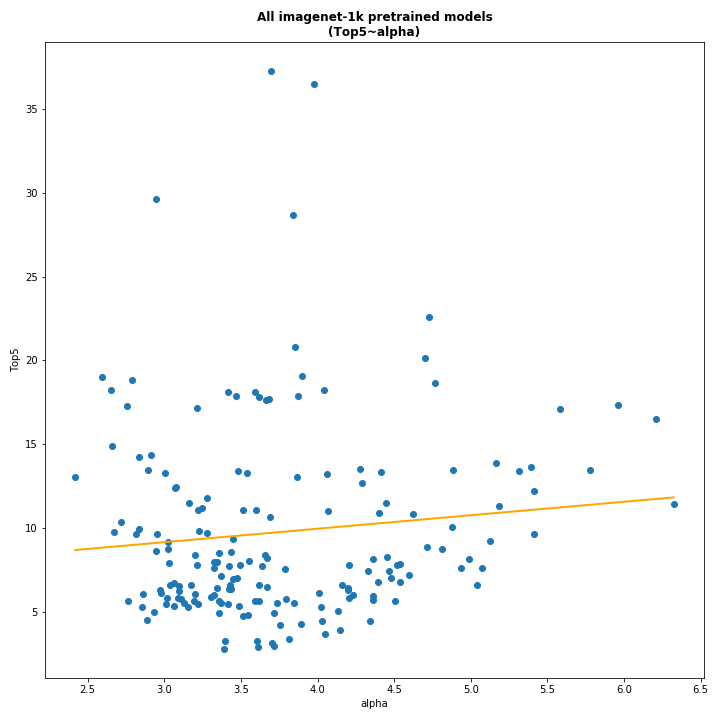
\includegraphics[width=4.9cm]{img/all-imagenet-1k_alpha.png}
        \label{fig:imagenet1k-alpha}
    }
    \qquad
    \subfigure[ CIFAR 10 ]{
        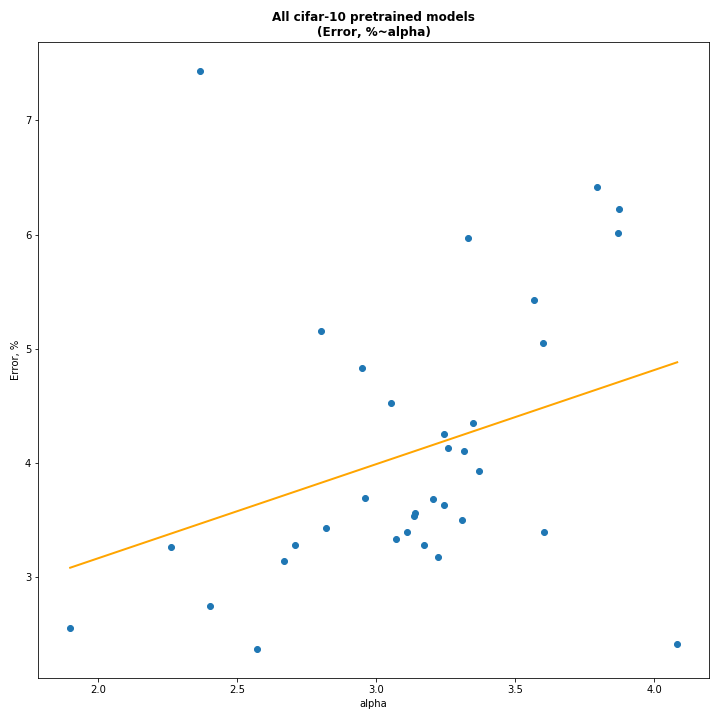
\includegraphics[width=4.9cm]{img/all-cifar-10_alpha.png}
        \label{fig:cifar10.alpha}
    }
    \qquad
    \subfigure[ CIFAR 100 ]{
        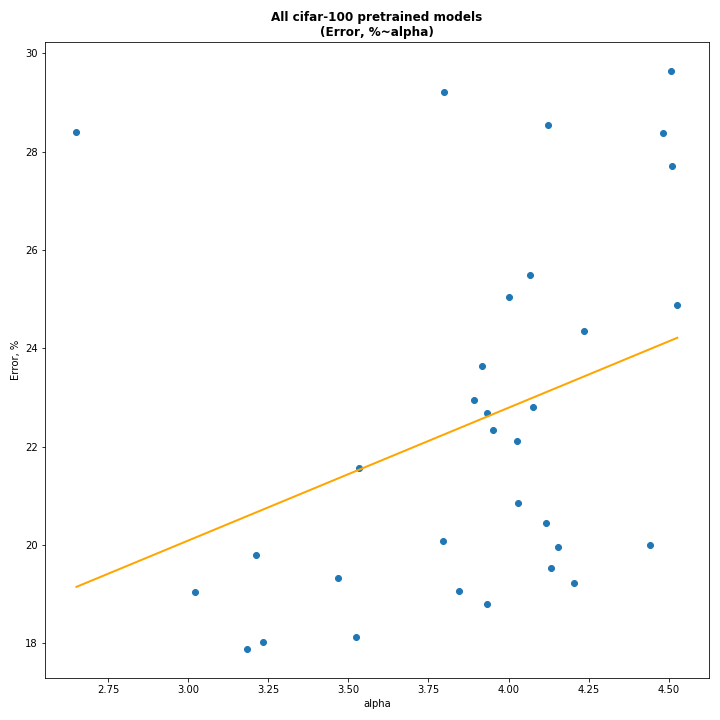
\includegraphics[width=4.9cm]{img/all-cifar-100_alpha.png}
        \label{fig:cifar100.alpha}
    }
    \qquad
    \subfigure[ SVHN ]{
        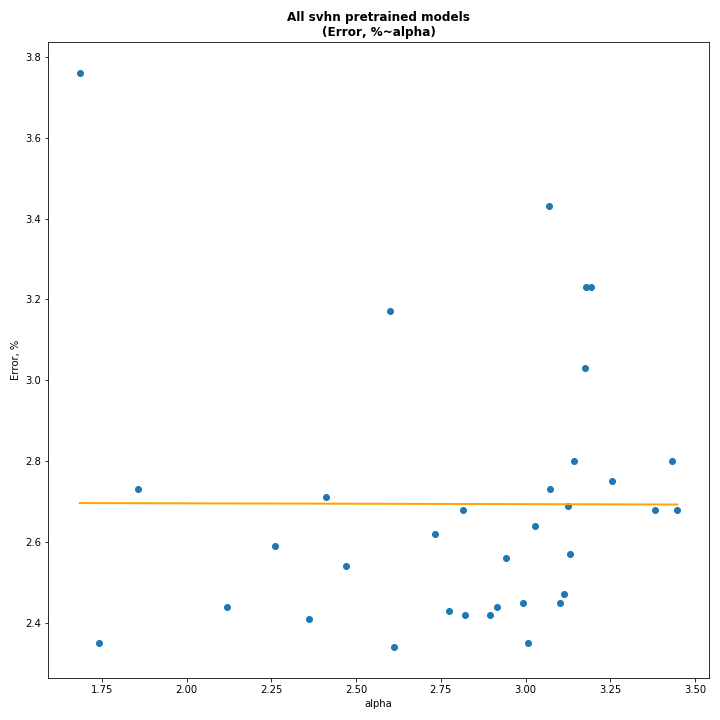
\includegraphics[width=4.9cm]{img/all-svhn_alpha.png}
        \label{fig:svhn.alpha}
    }
    \qquad
    \subfigure[ CUB 200 ]{
        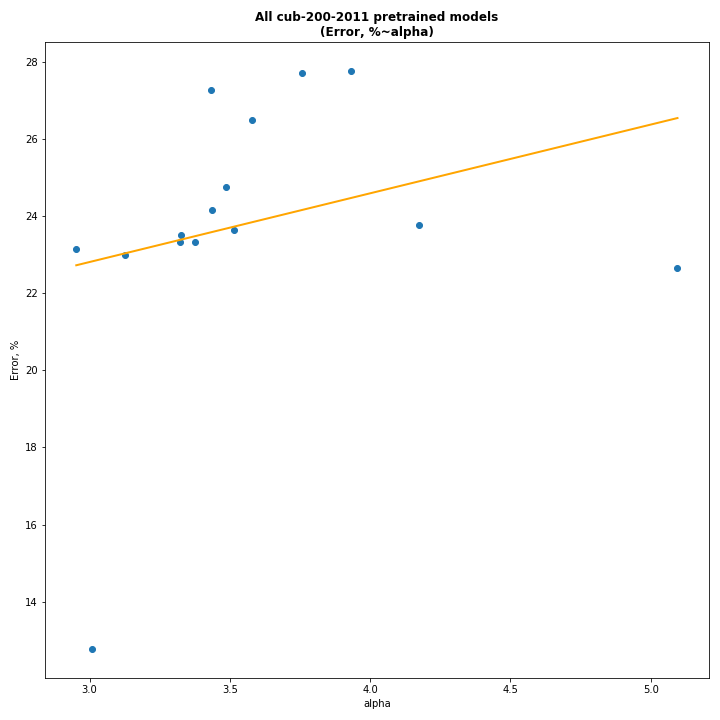
\includegraphics[width=4.9cm]{img/all-cub-200-2011_alpha.png}
        \label{fig:cub200.alpha}
    }
    \caption{PL exponent $\alpha$ versus reported Top1 Test Accuracies for pretrained DNNs available for different datasets (as segmented in Table~\ref{table:datasets}).
            }
    \label{fig:DSalphas}
\end{figure}

 
\begin{figure}[t]
    \centering
    \subfigure[ ResNet ]{
        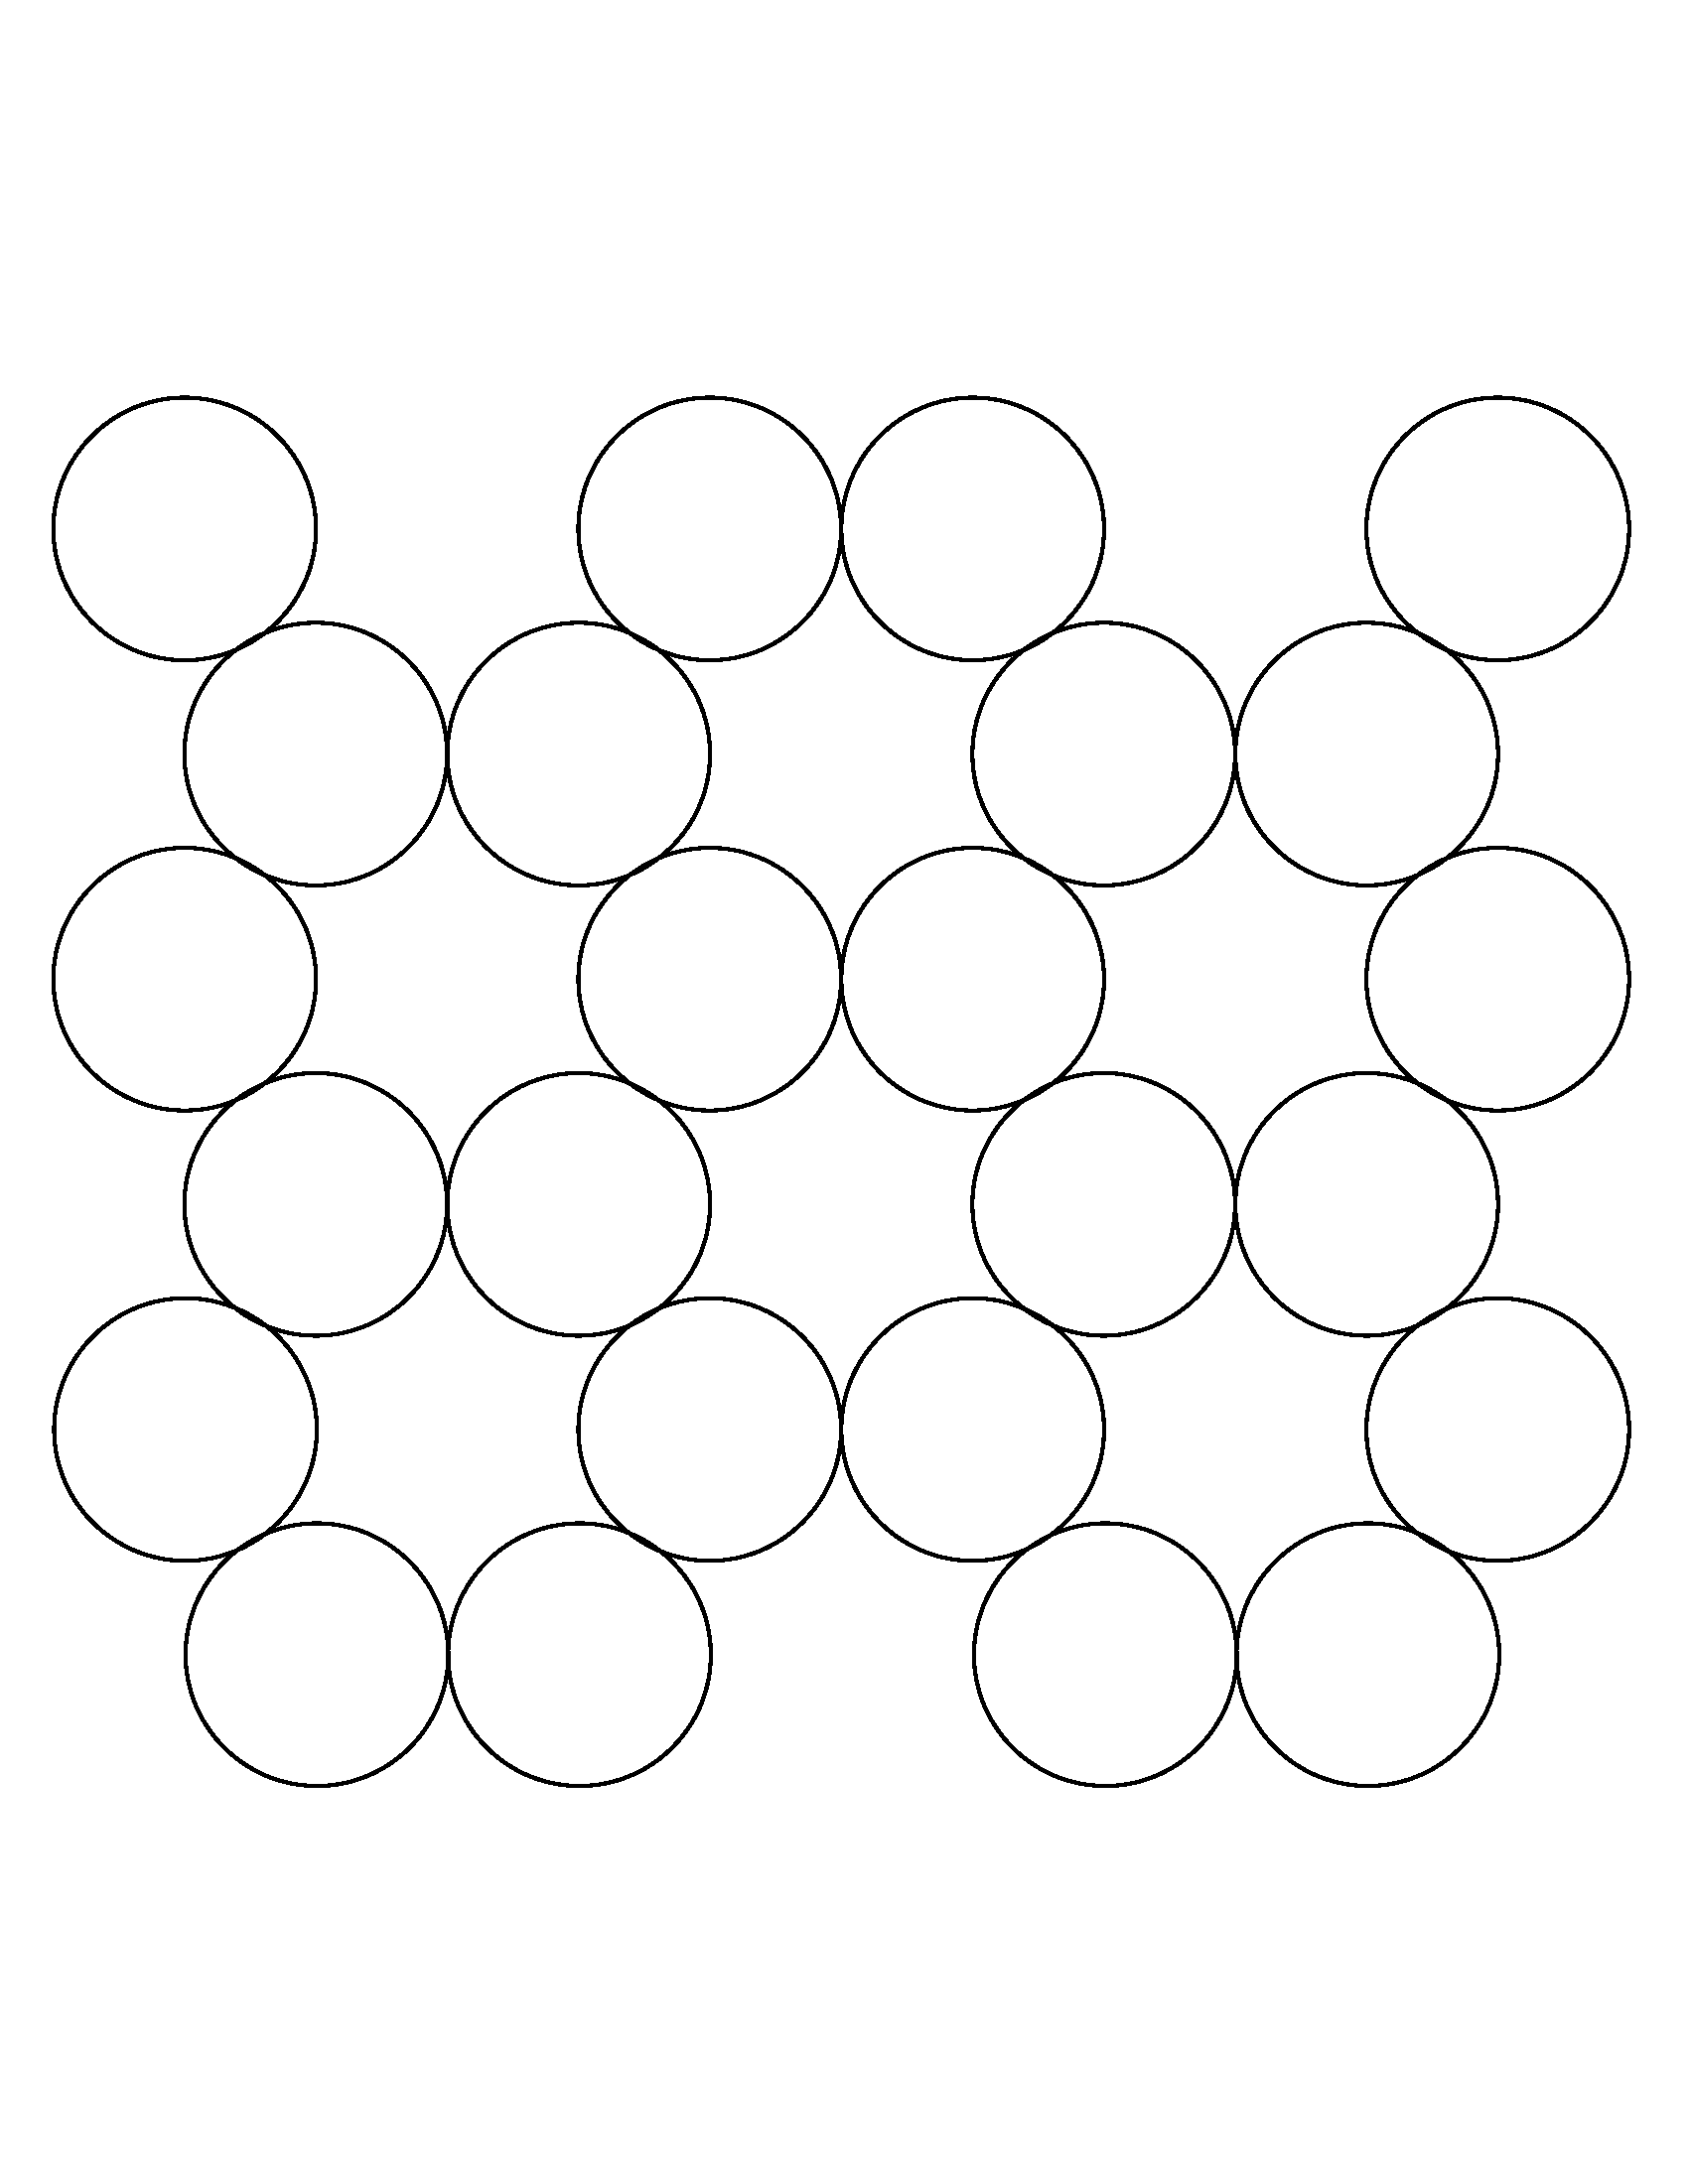
\includegraphics[width=2.7cm]{img/hex.png}
        \label{fig:ARCHalphas_01}
    }
    \subfigure[ SENet/SE-ResNet/SE-PreResNet/SE-ResNeXt ]{
        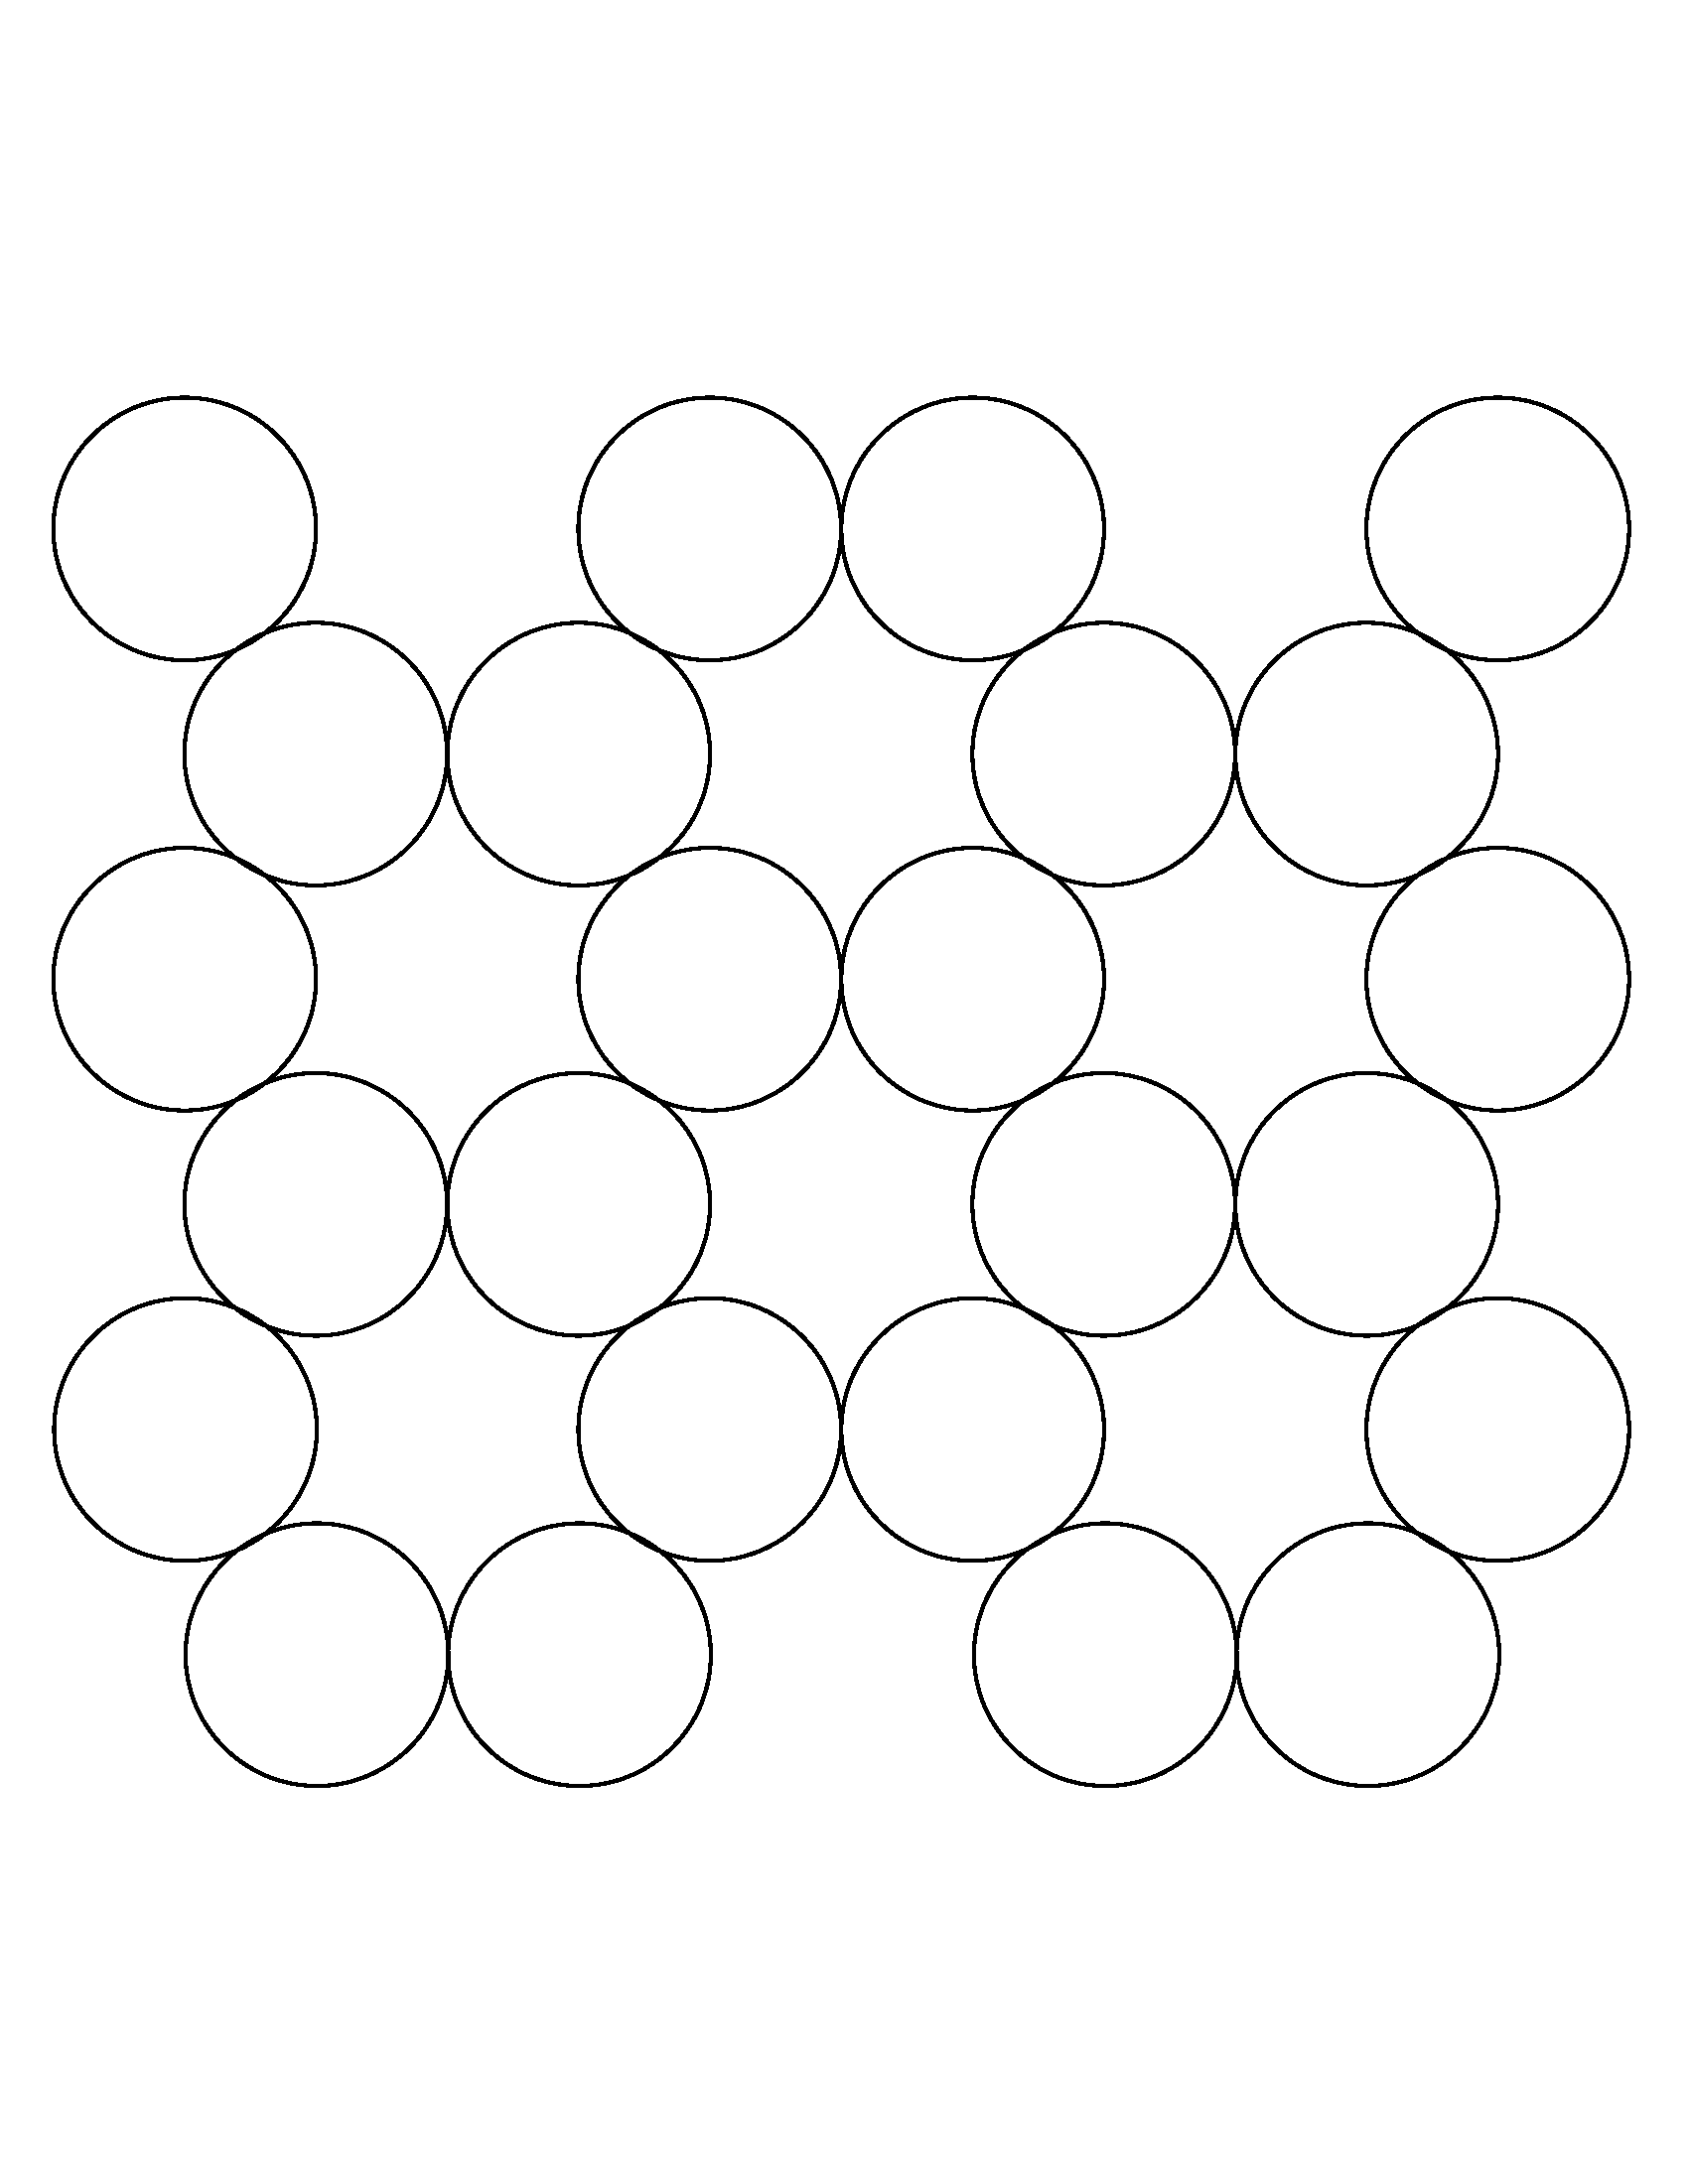
\includegraphics[width=2.7cm]{img/hex.png}
        \label{fig:ARCHalphas_02}
    }
    \subfigure[ DIA-ResNet/DIA-PreResNet ]{
        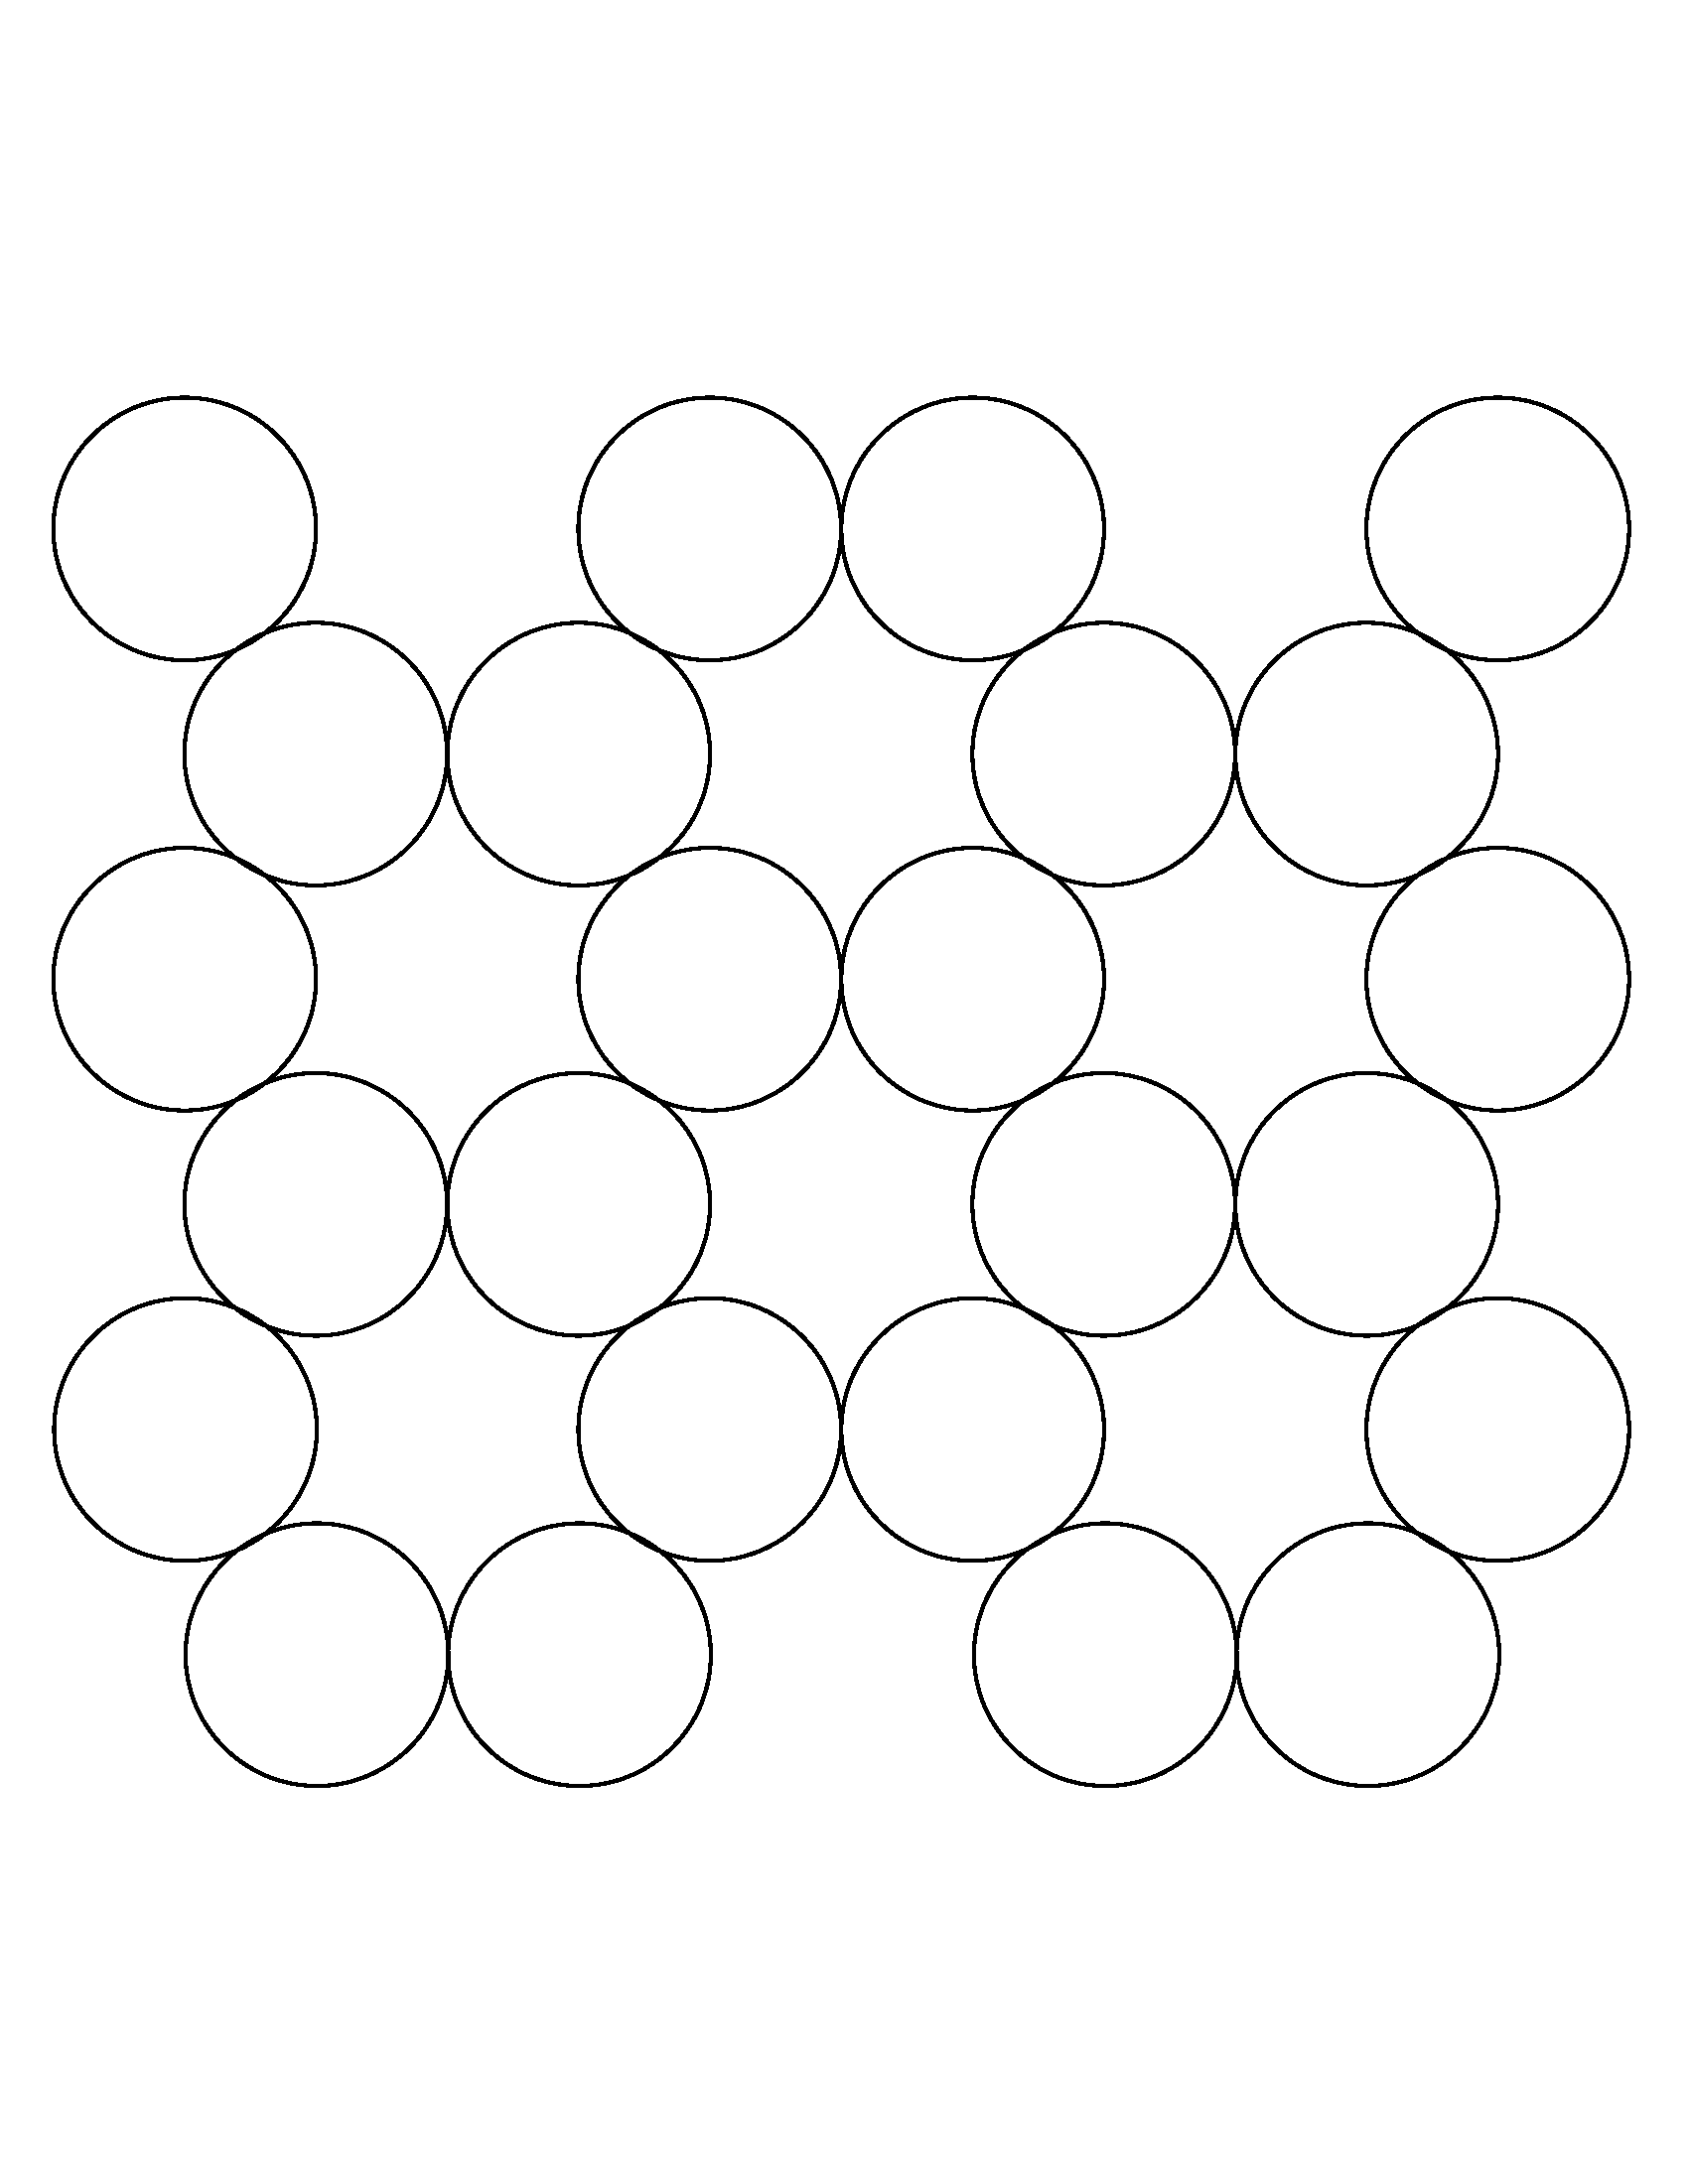
\includegraphics[width=2.7cm]{img/hex.png}
        \label{fig:ARCHalphas_03}
    }
    \subfigure[ ResNeXt ]{
        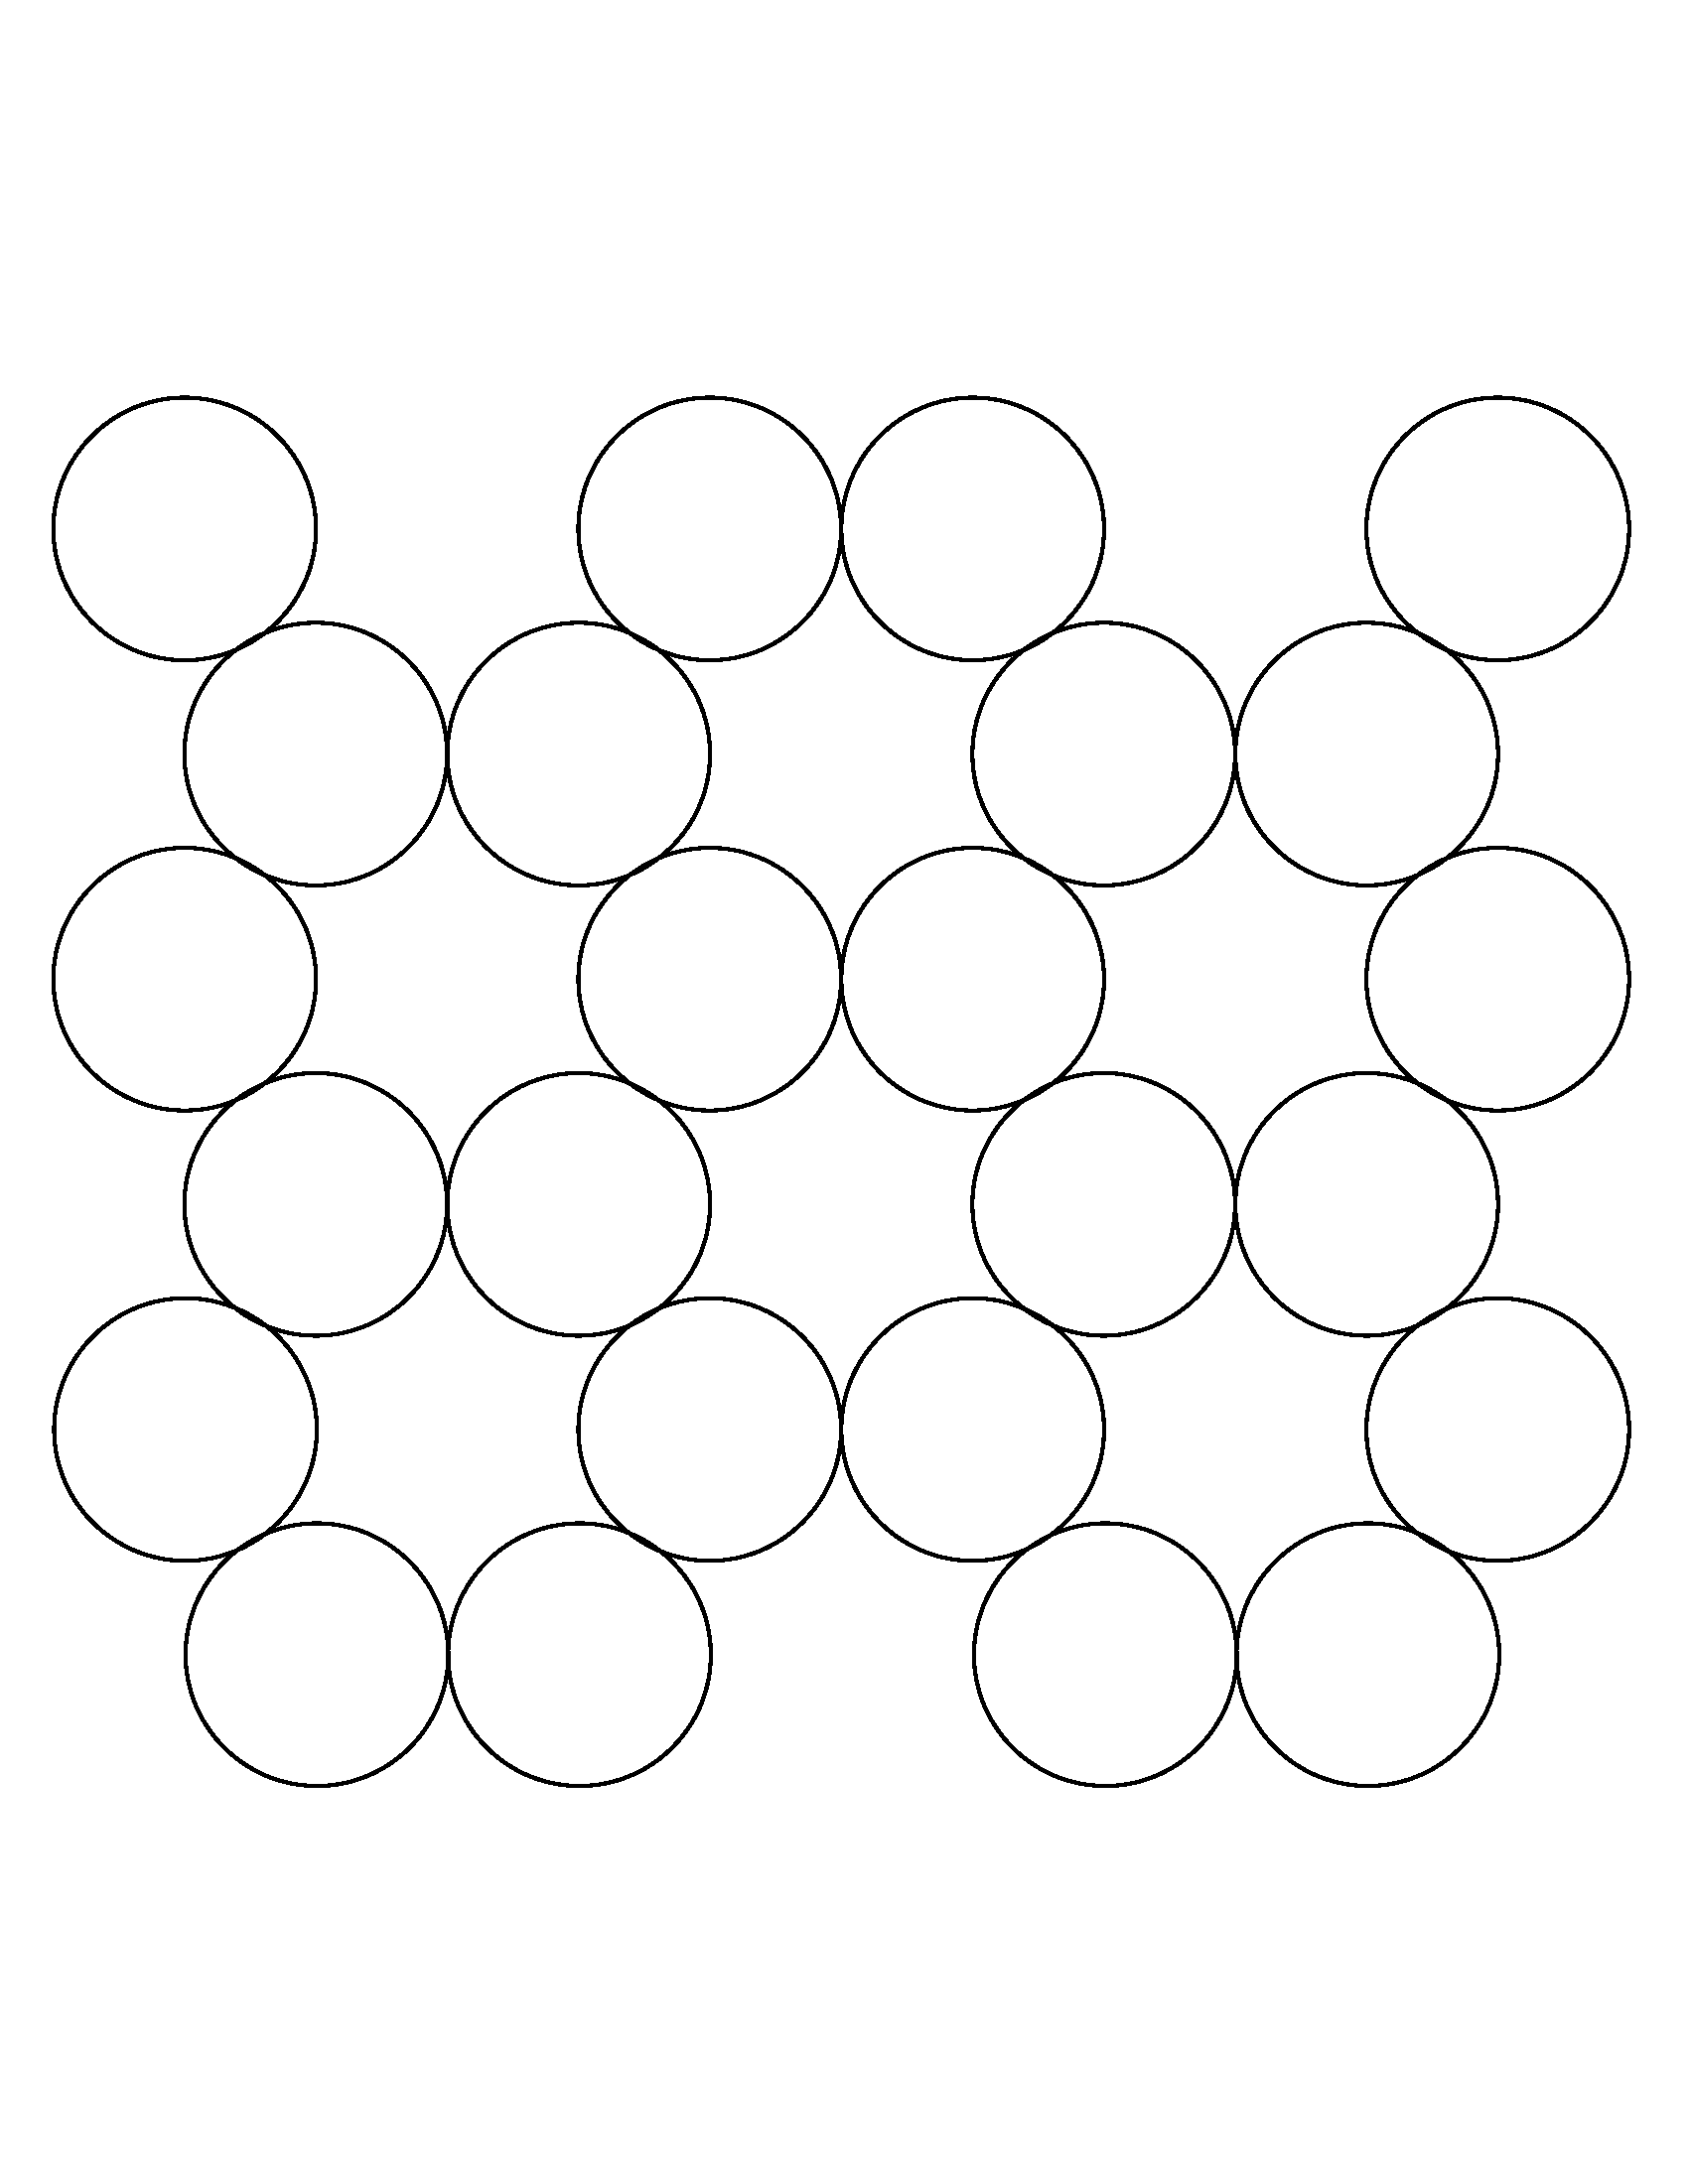
\includegraphics[width=2.7cm]{img/hex.png}
        \label{fig:ARCHalphas_04}
    }
    \subfigure[ WRN ]{
        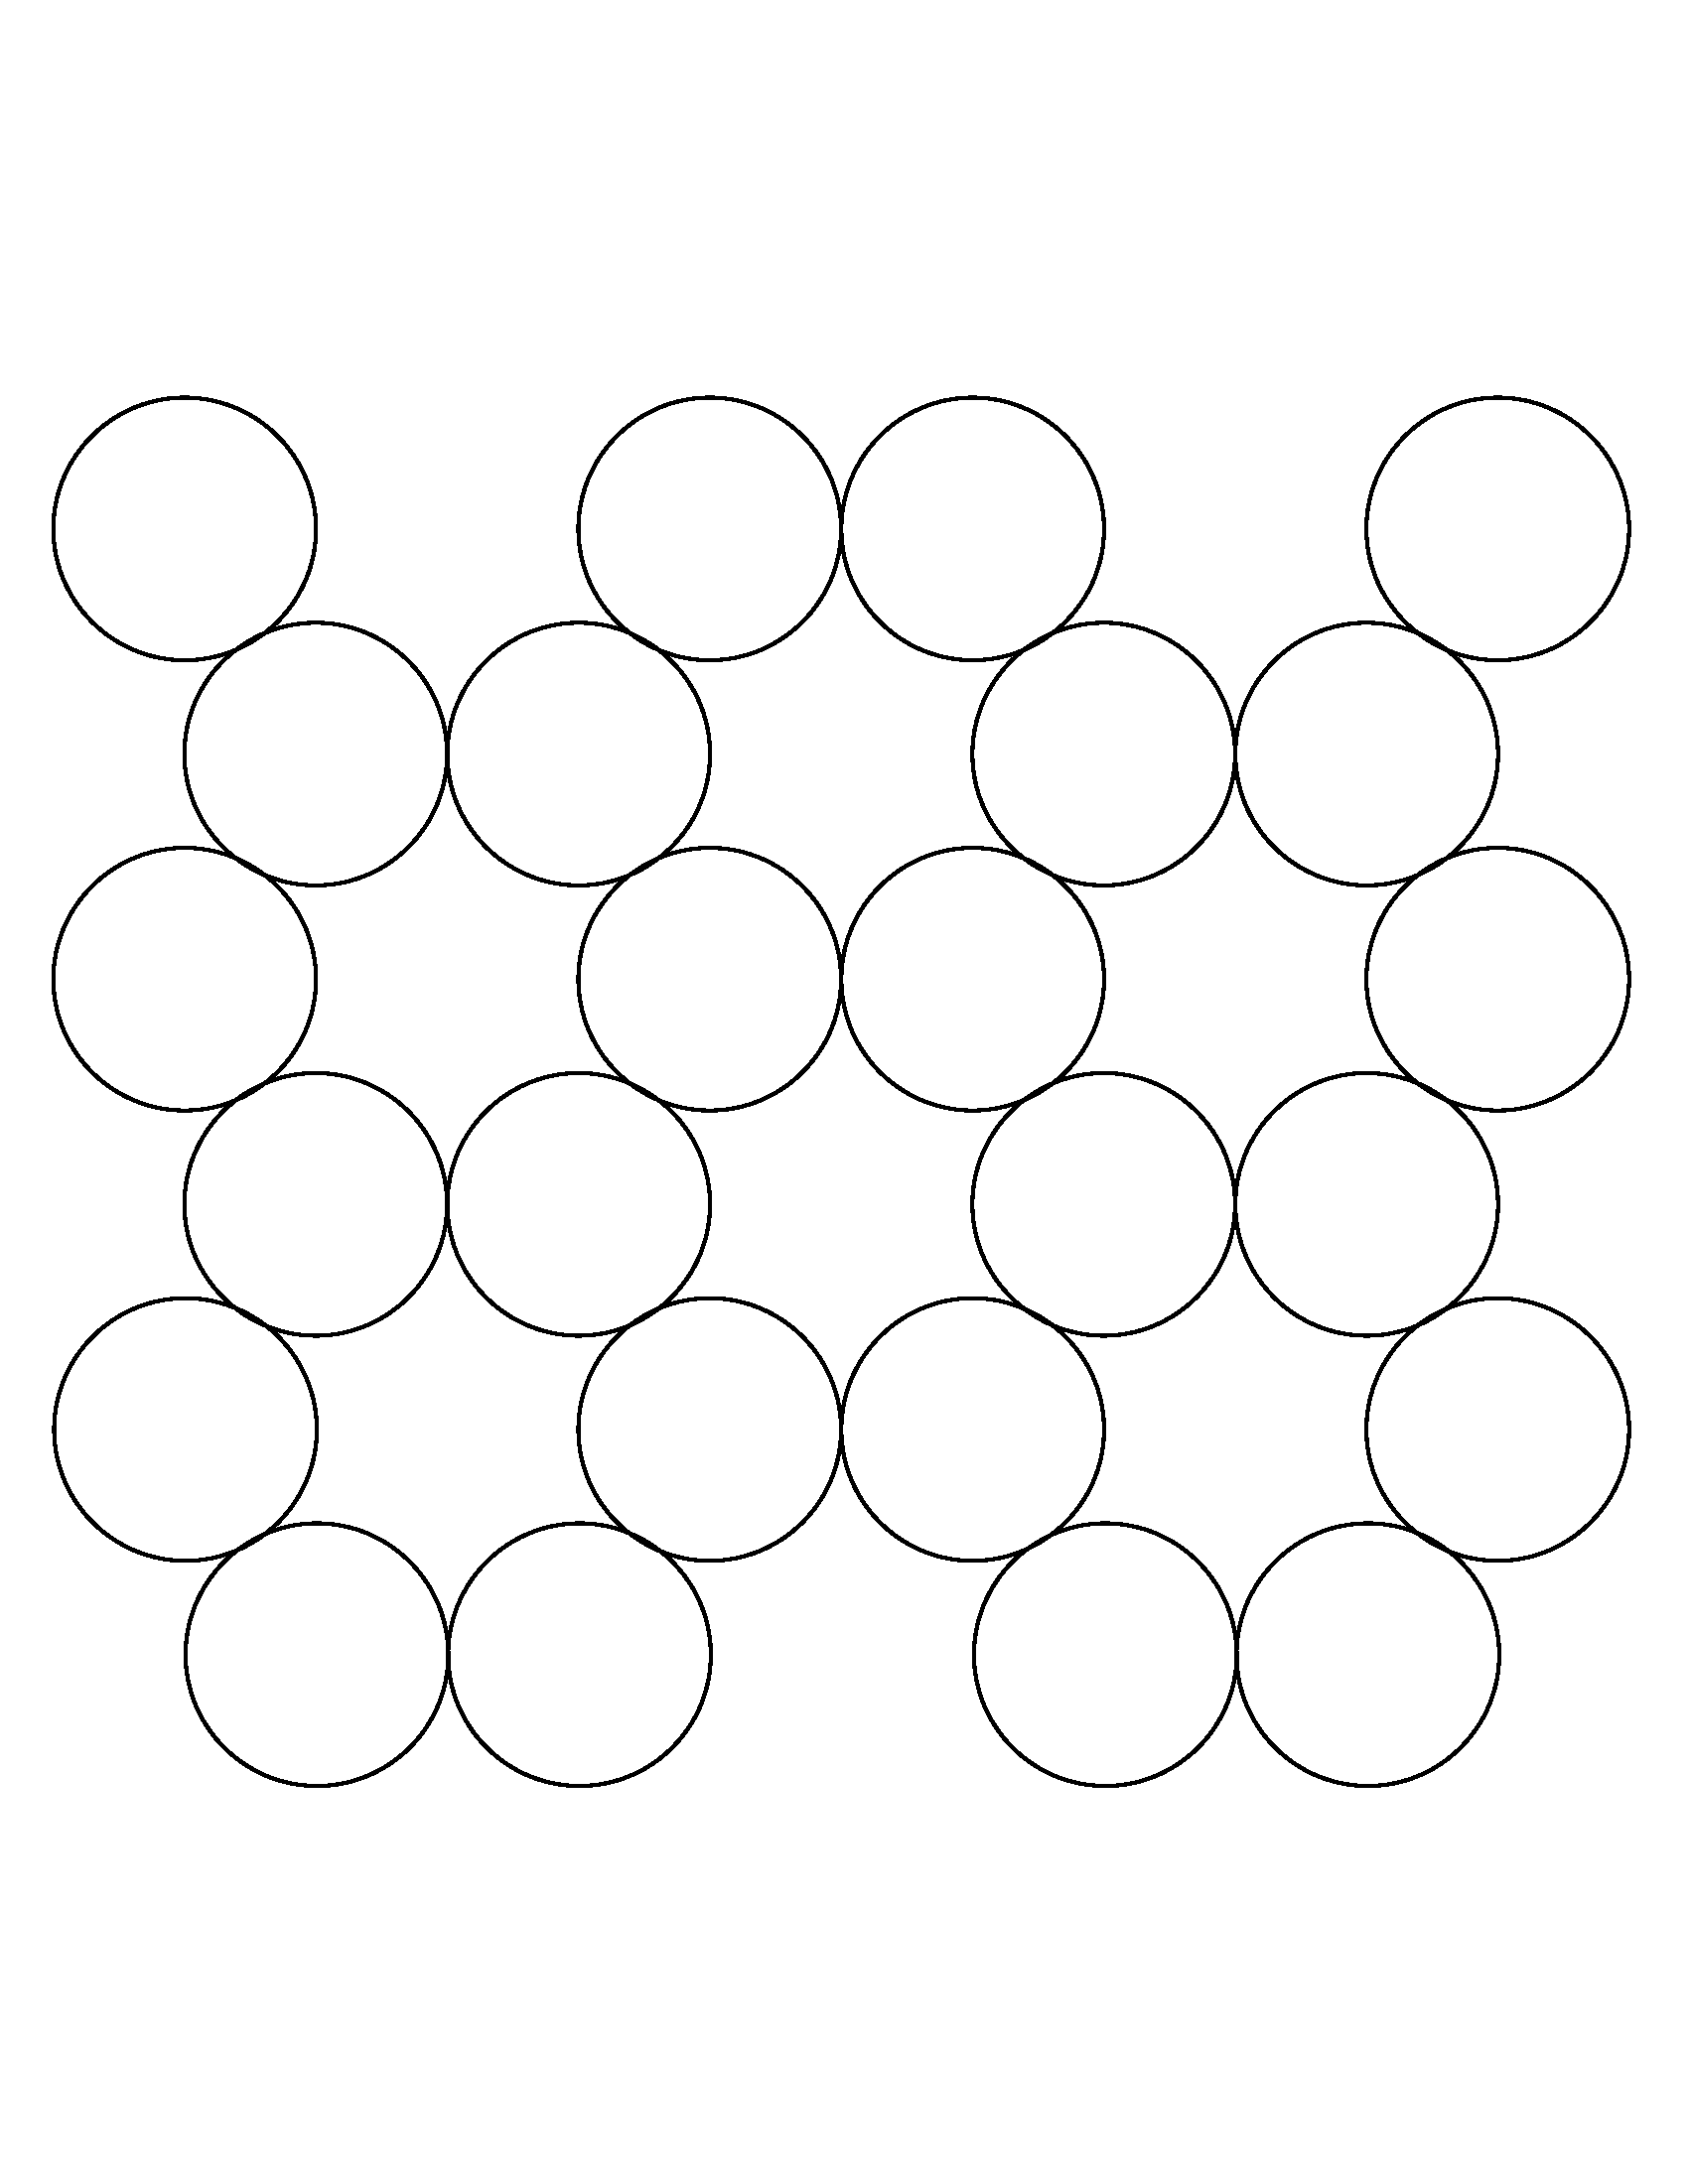
\includegraphics[width=2.7cm]{img/hex.png}
        \label{fig:ARCHalphas_05}
    }
    \subfigure[ DLA ]{
        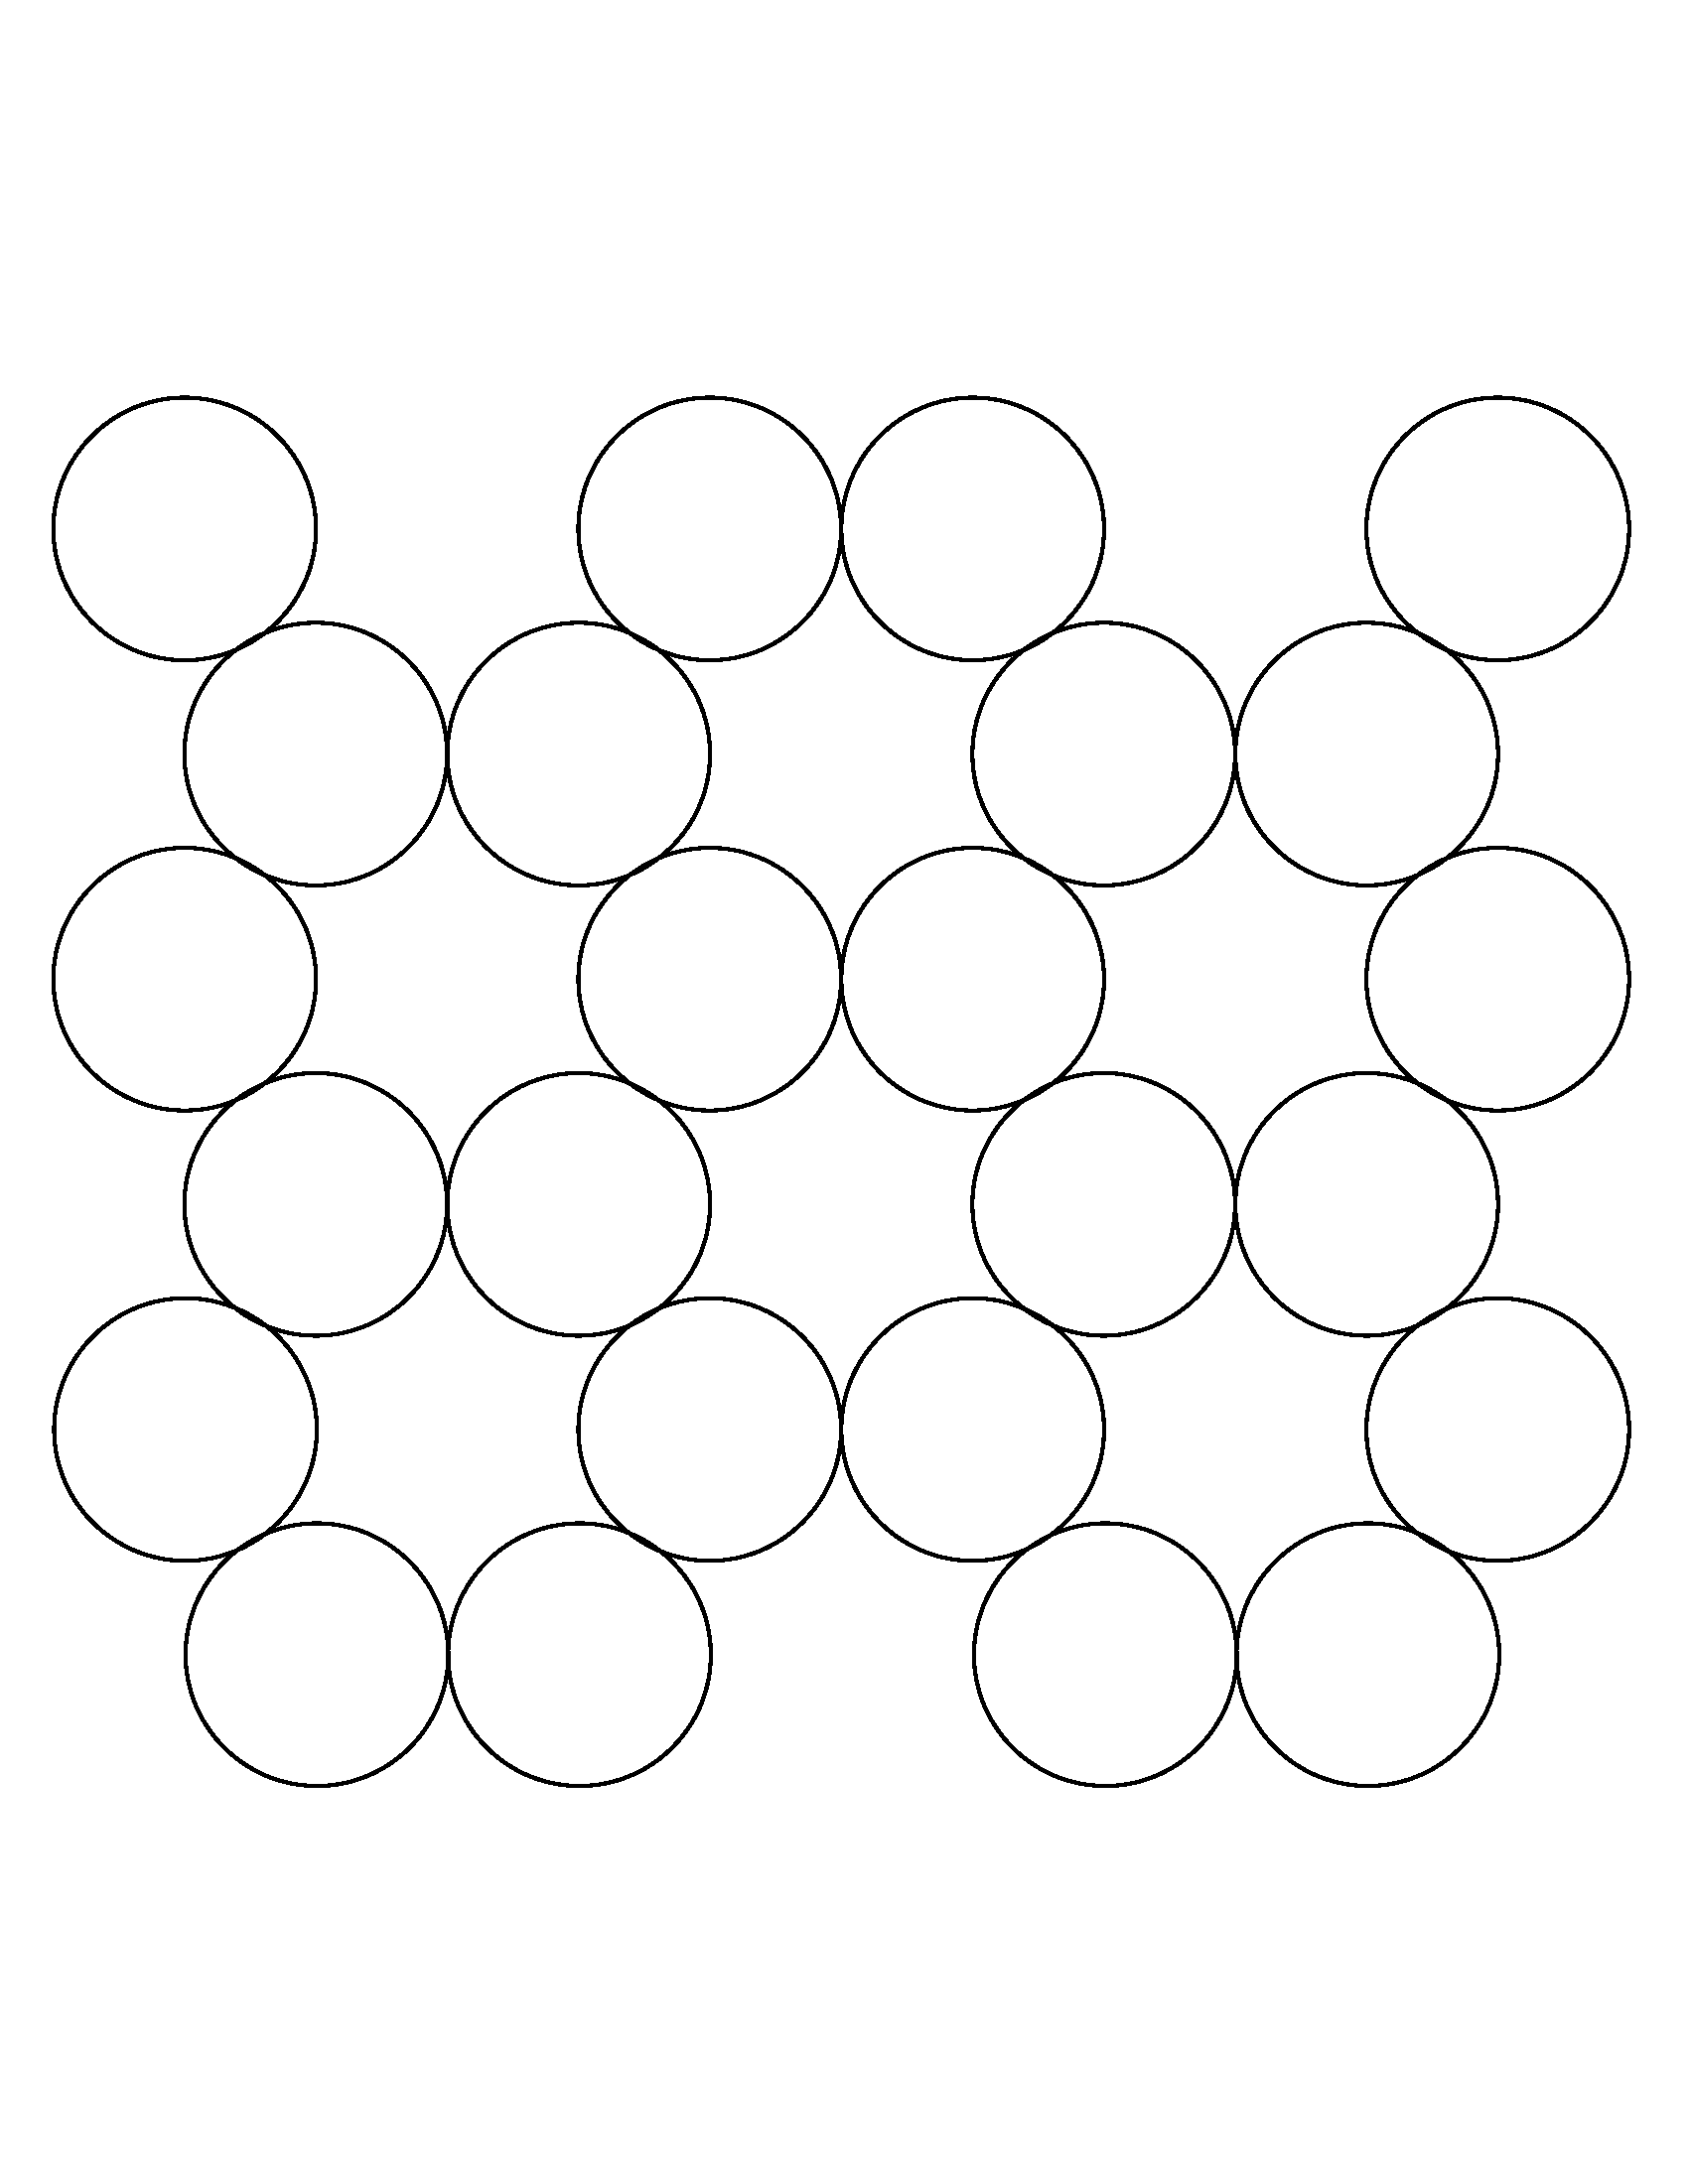
\includegraphics[width=2.7cm]{img/hex.png}
        \label{fig:ARCHalphas_06}
    }
    \subfigure[ PreResNet ]{
        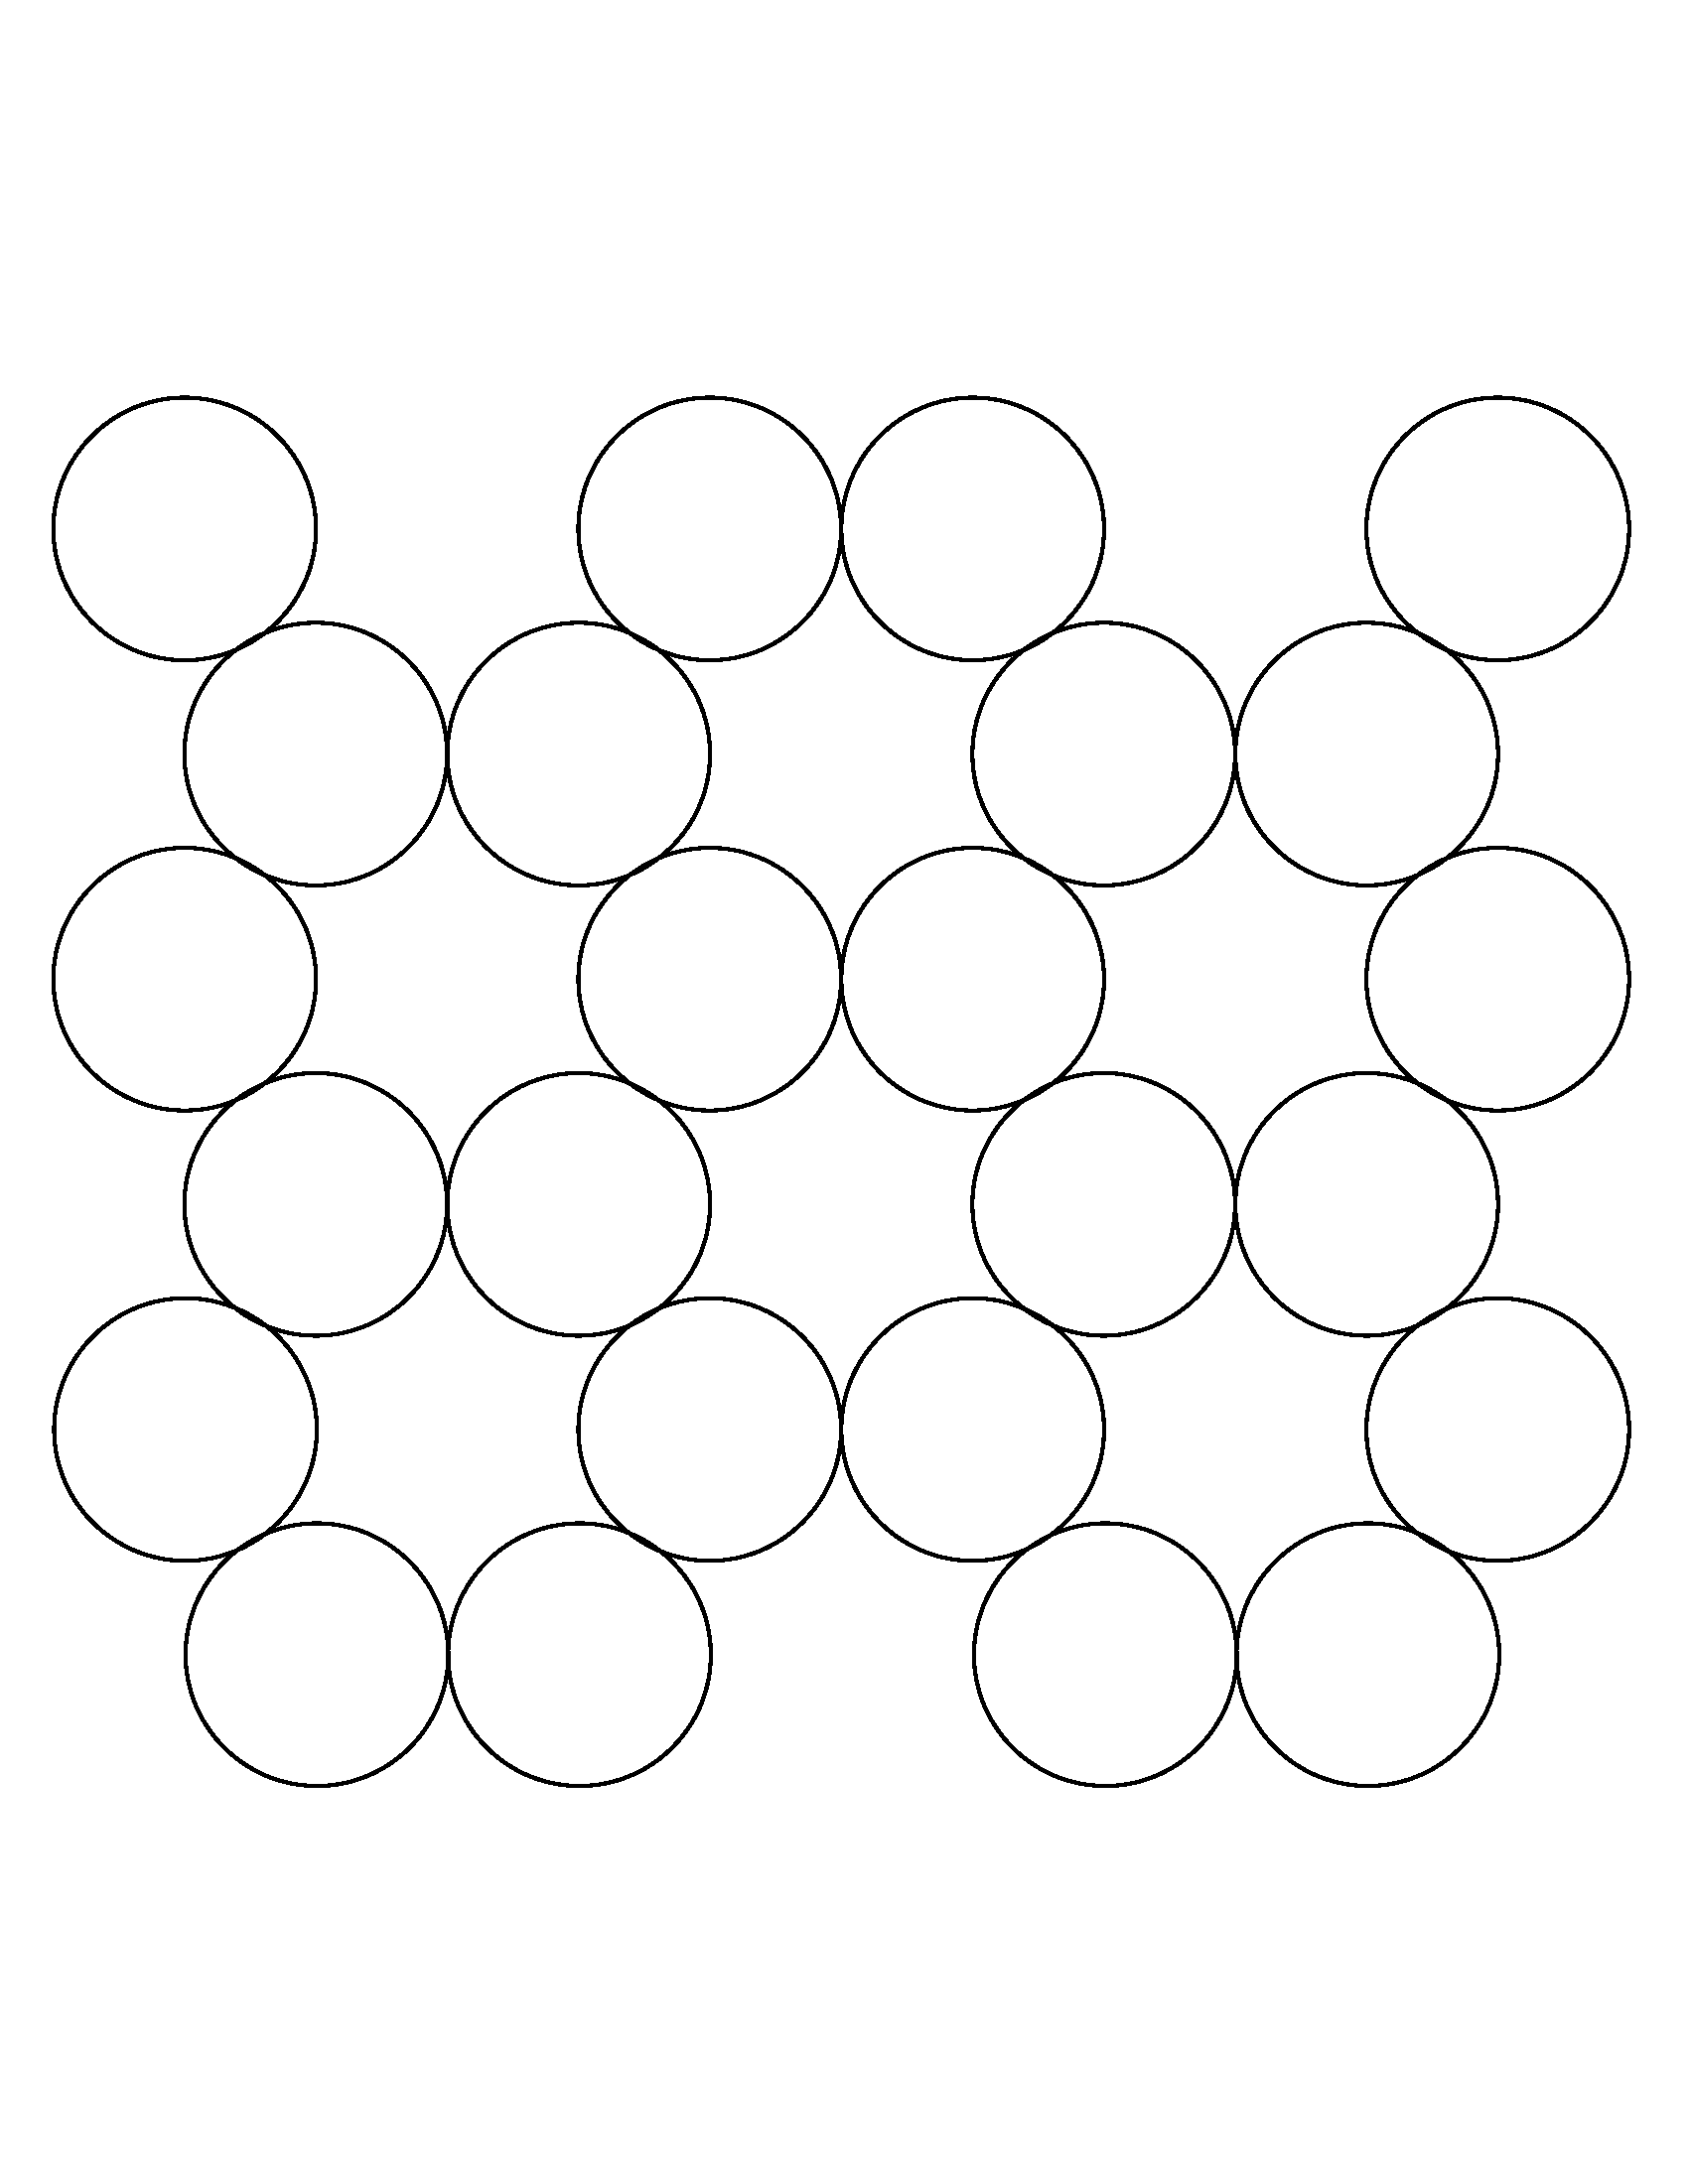
\includegraphics[width=2.7cm]{img/hex.png}
        \label{fig:ARCHalphas_07}
    }
    \subfigure[ ProxylessNAS ]{
        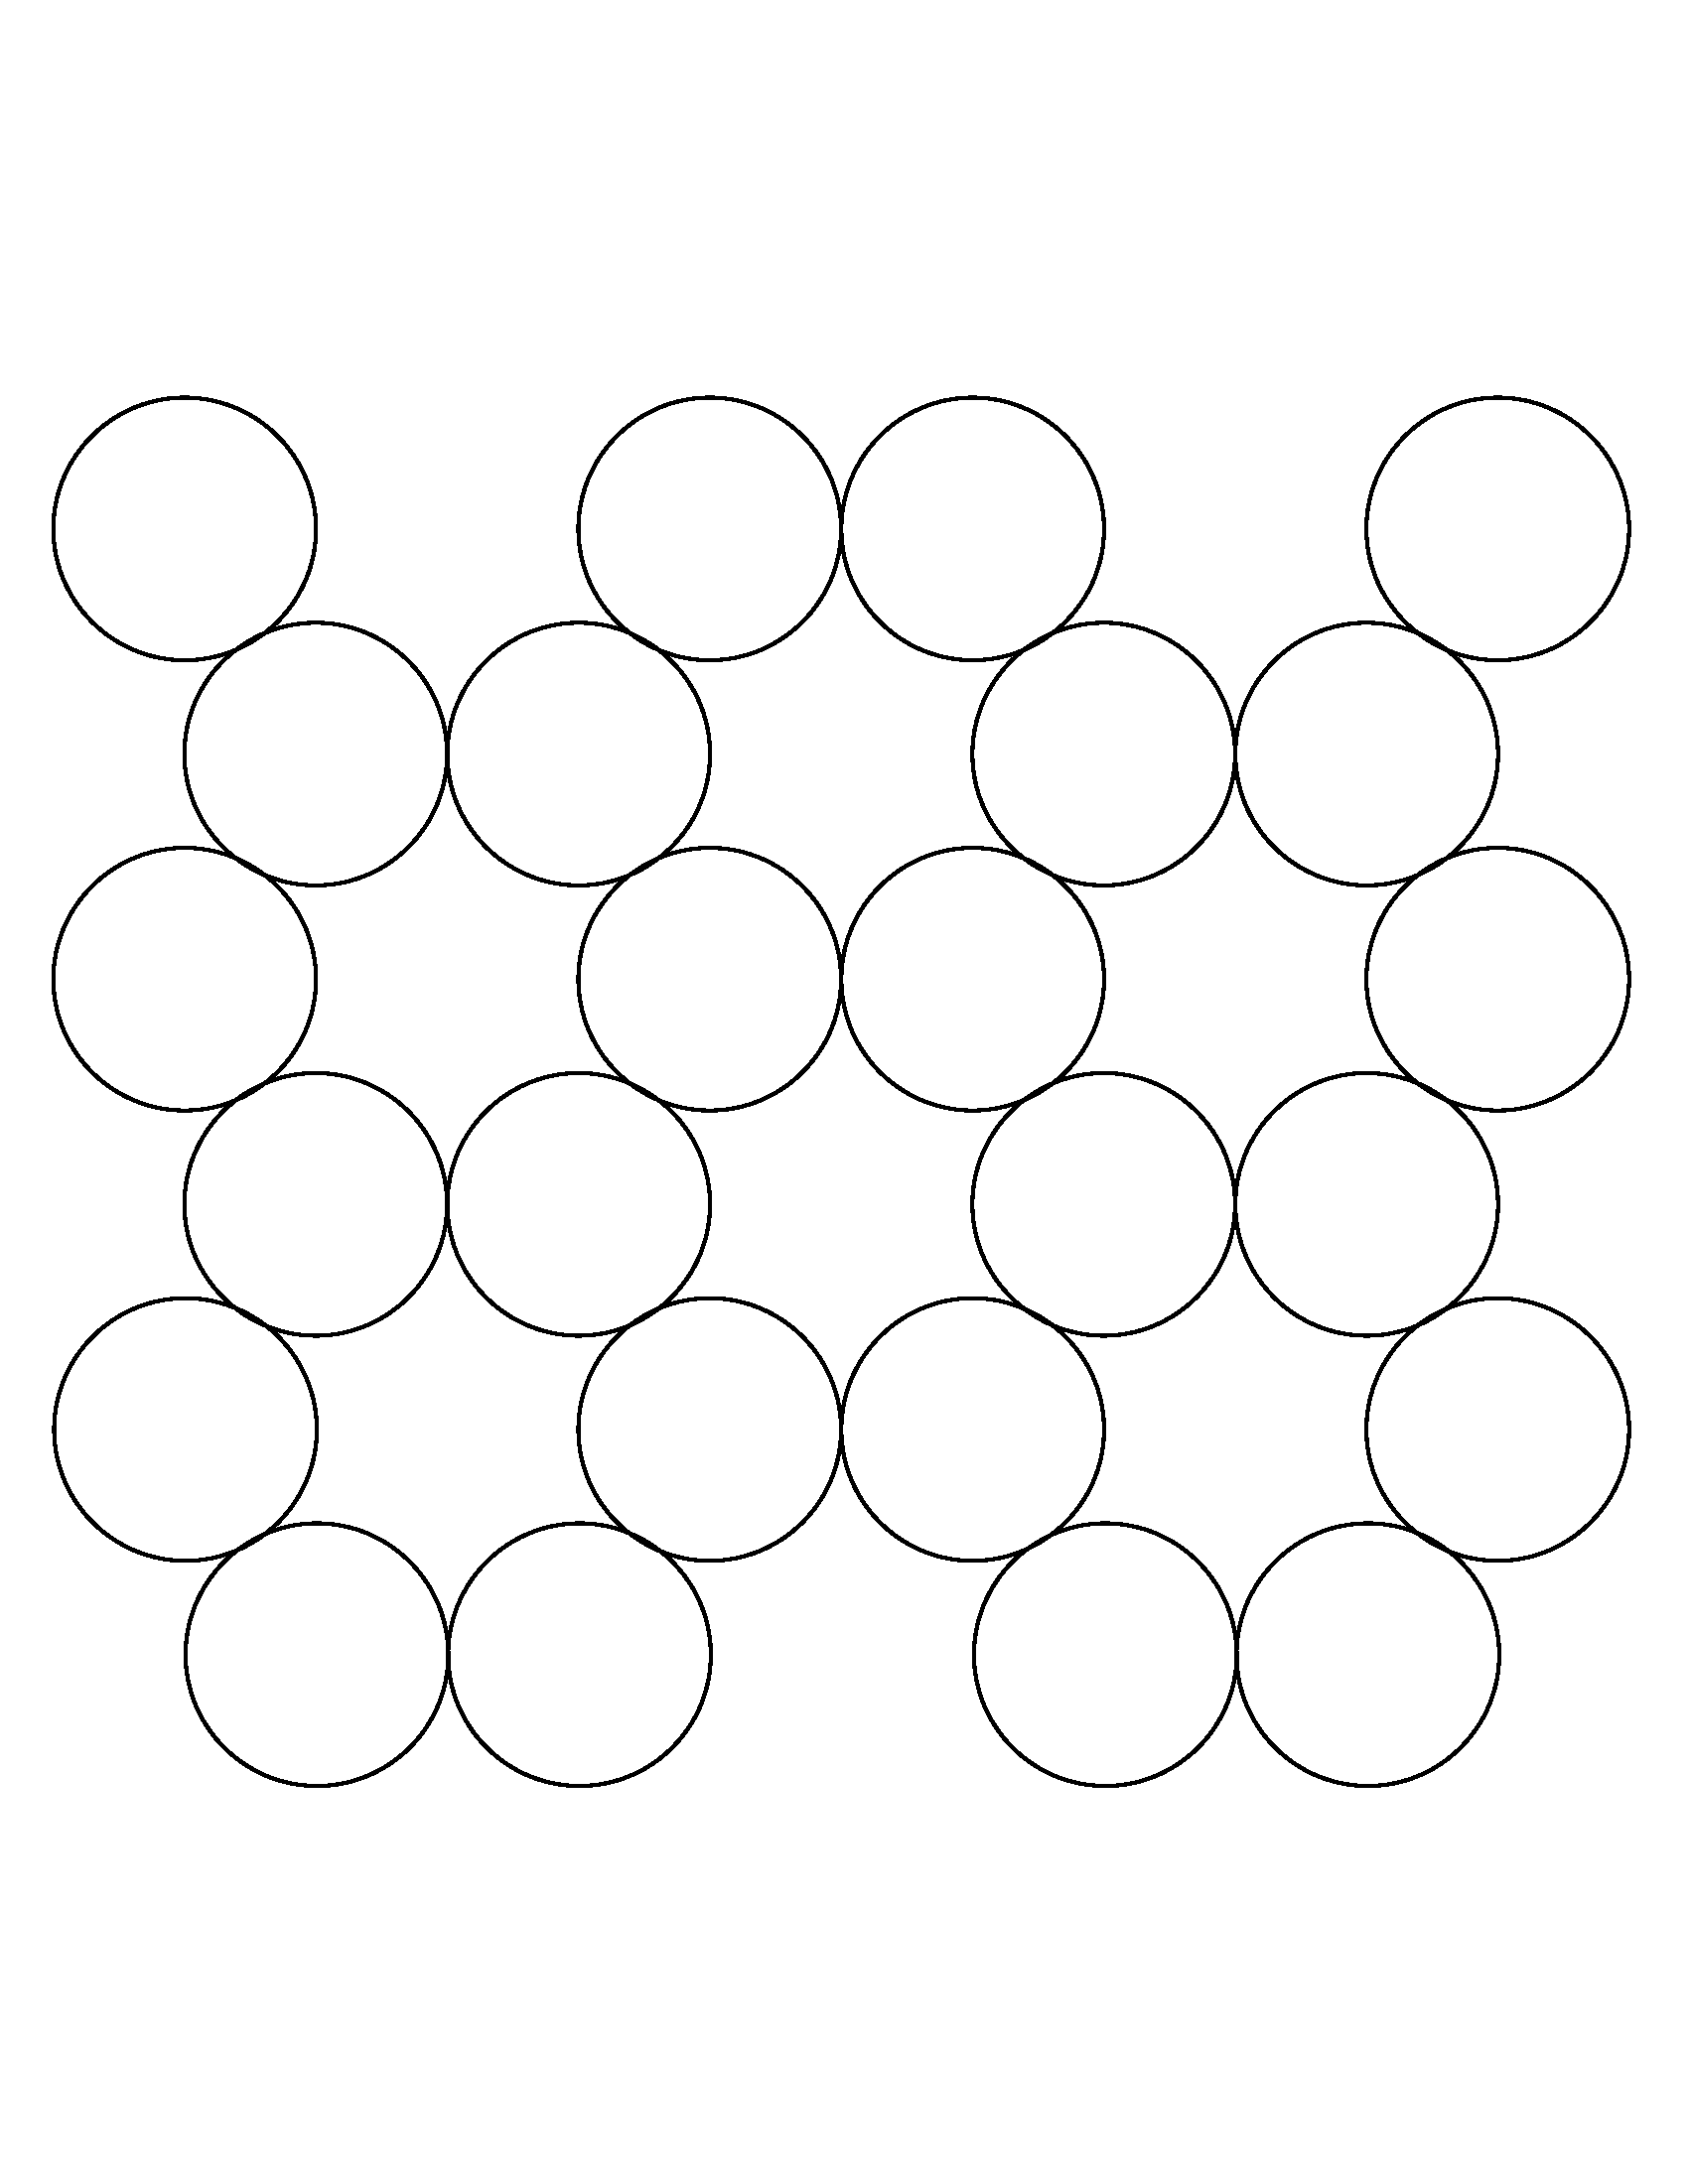
\includegraphics[width=2.7cm]{img/hex.png}
        \label{fig:ARCHalphas_08}
    }
    \subfigure[ VGG/BN-VGG ]{
        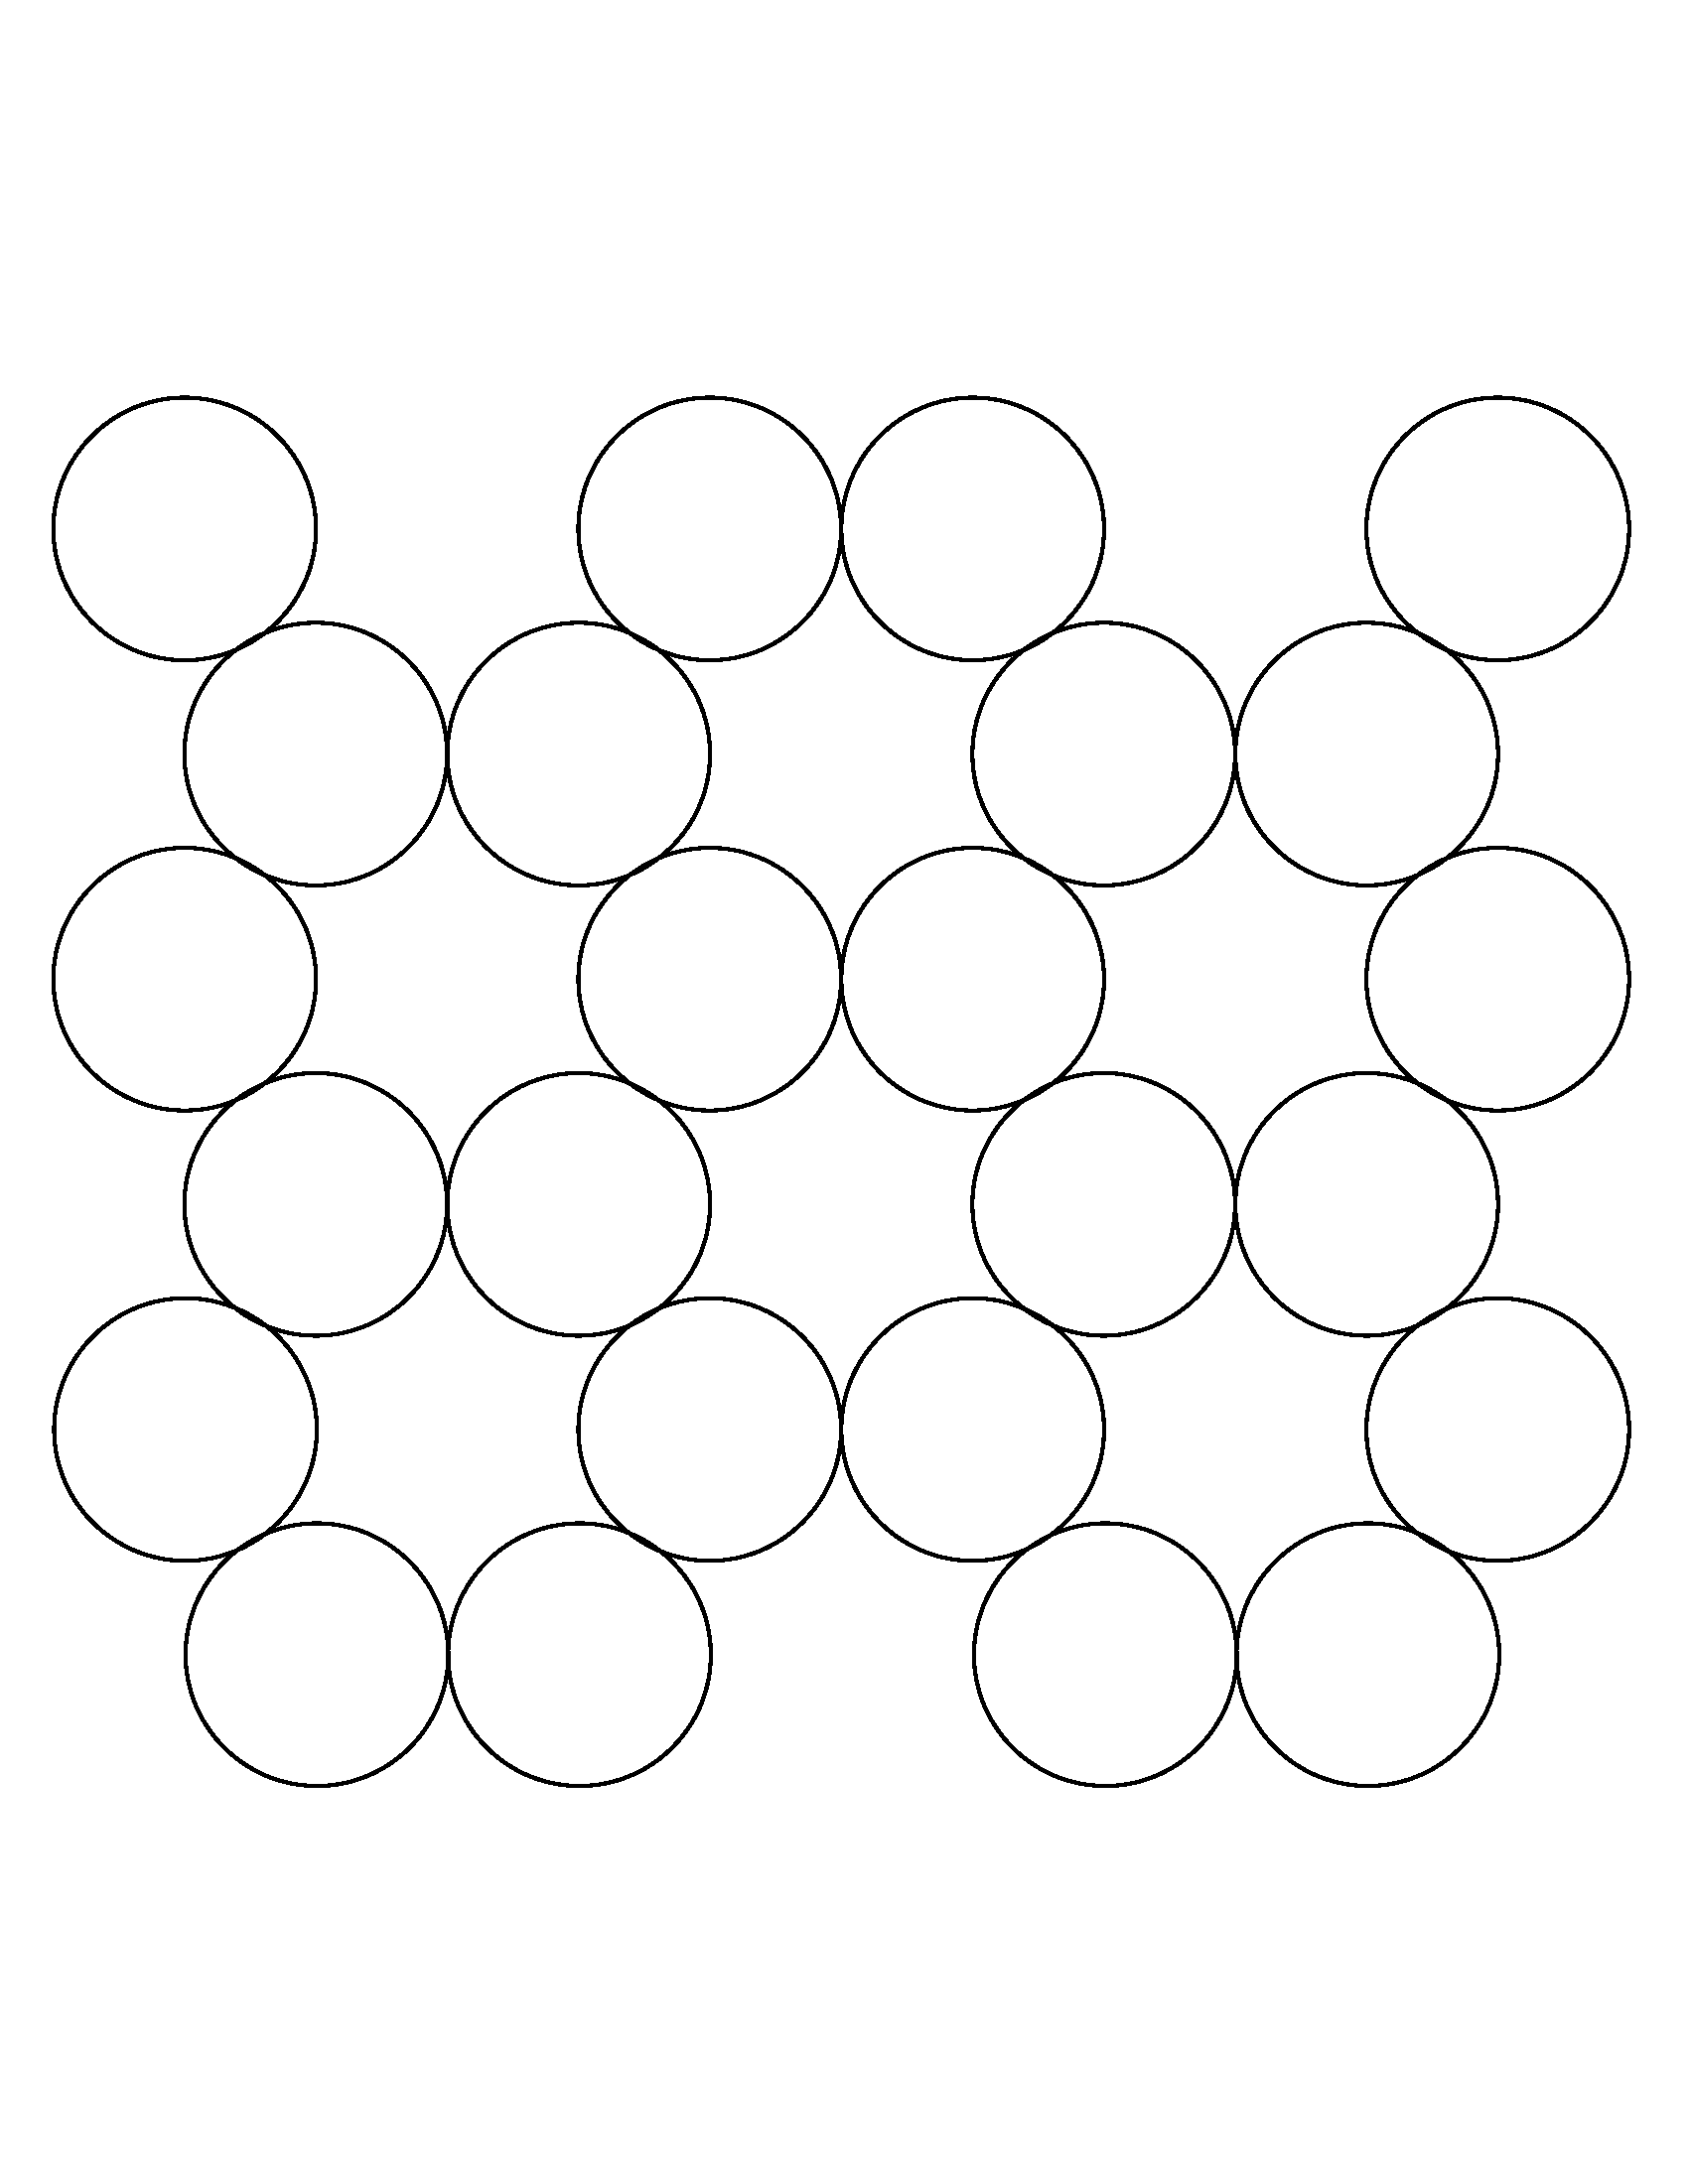
\includegraphics[width=2.7cm]{img/hex.png}
        \label{fig:ARCHalphas_09}
    }
    \subfigure[ IGCV3 ]{
        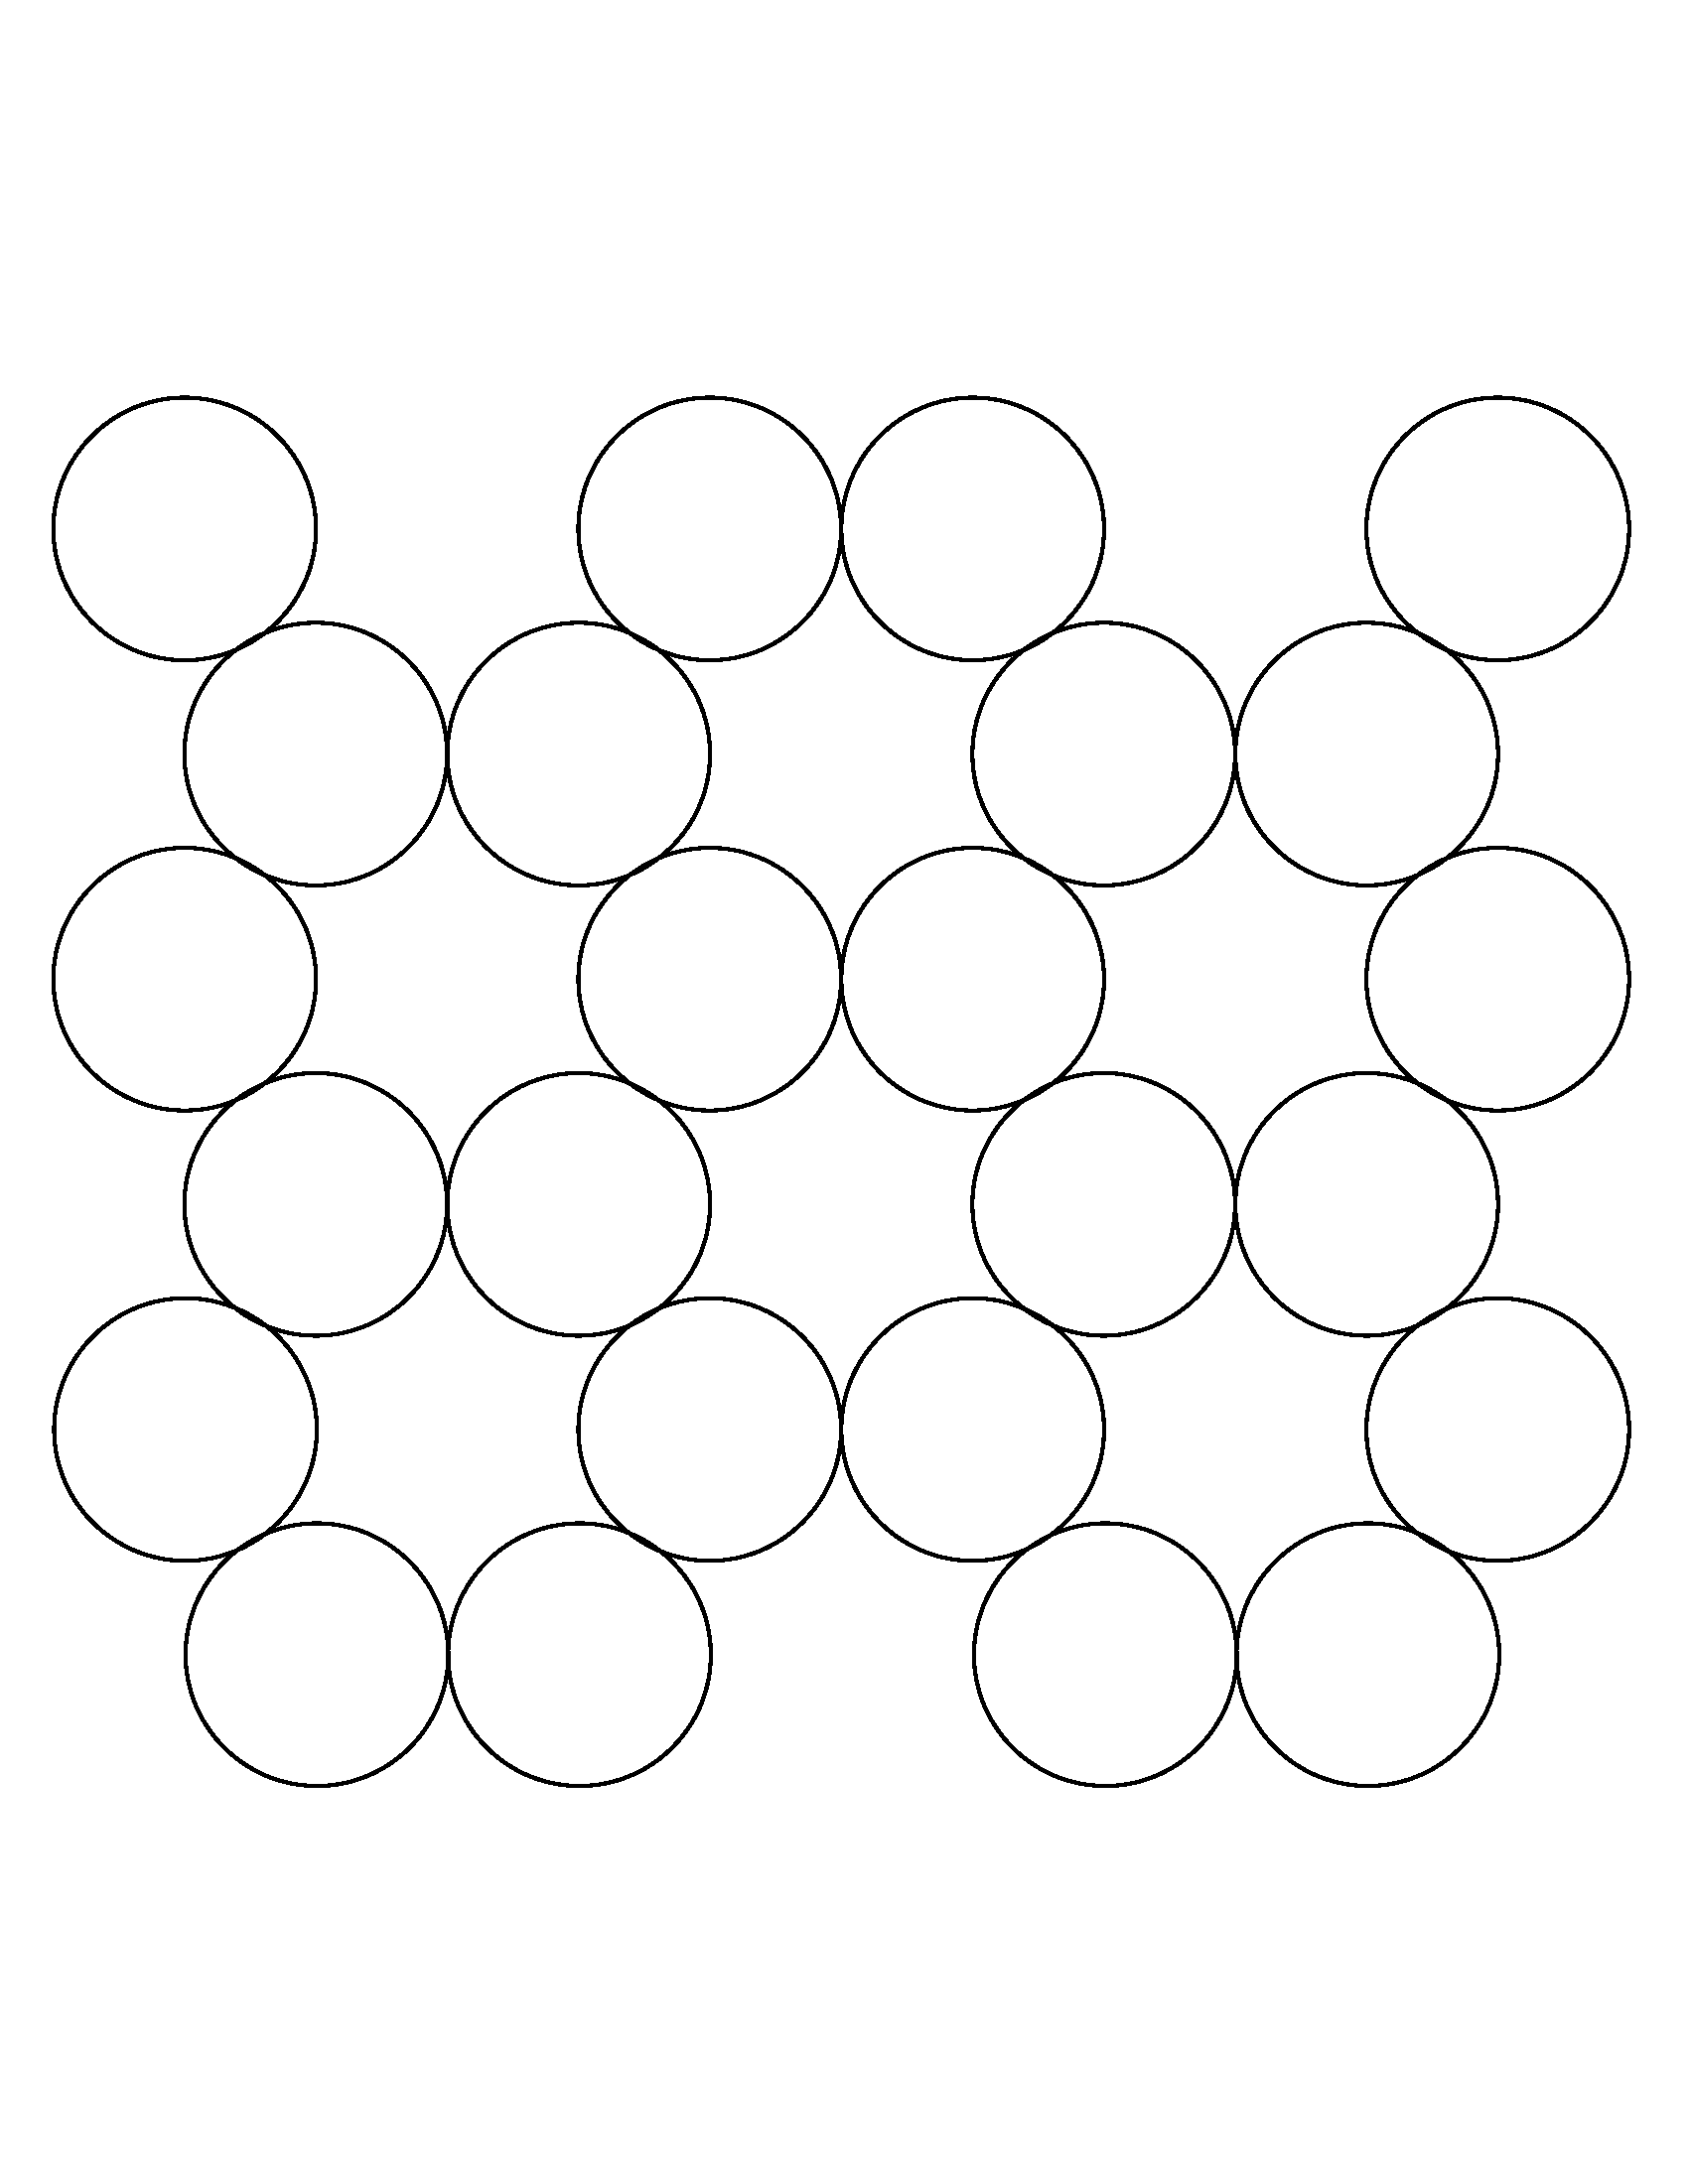
\includegraphics[width=2.7cm]{img/hex.png}
        \label{fig:ARCHalphas_10}
    }
    \subfigure[ EfficientNet ]{
        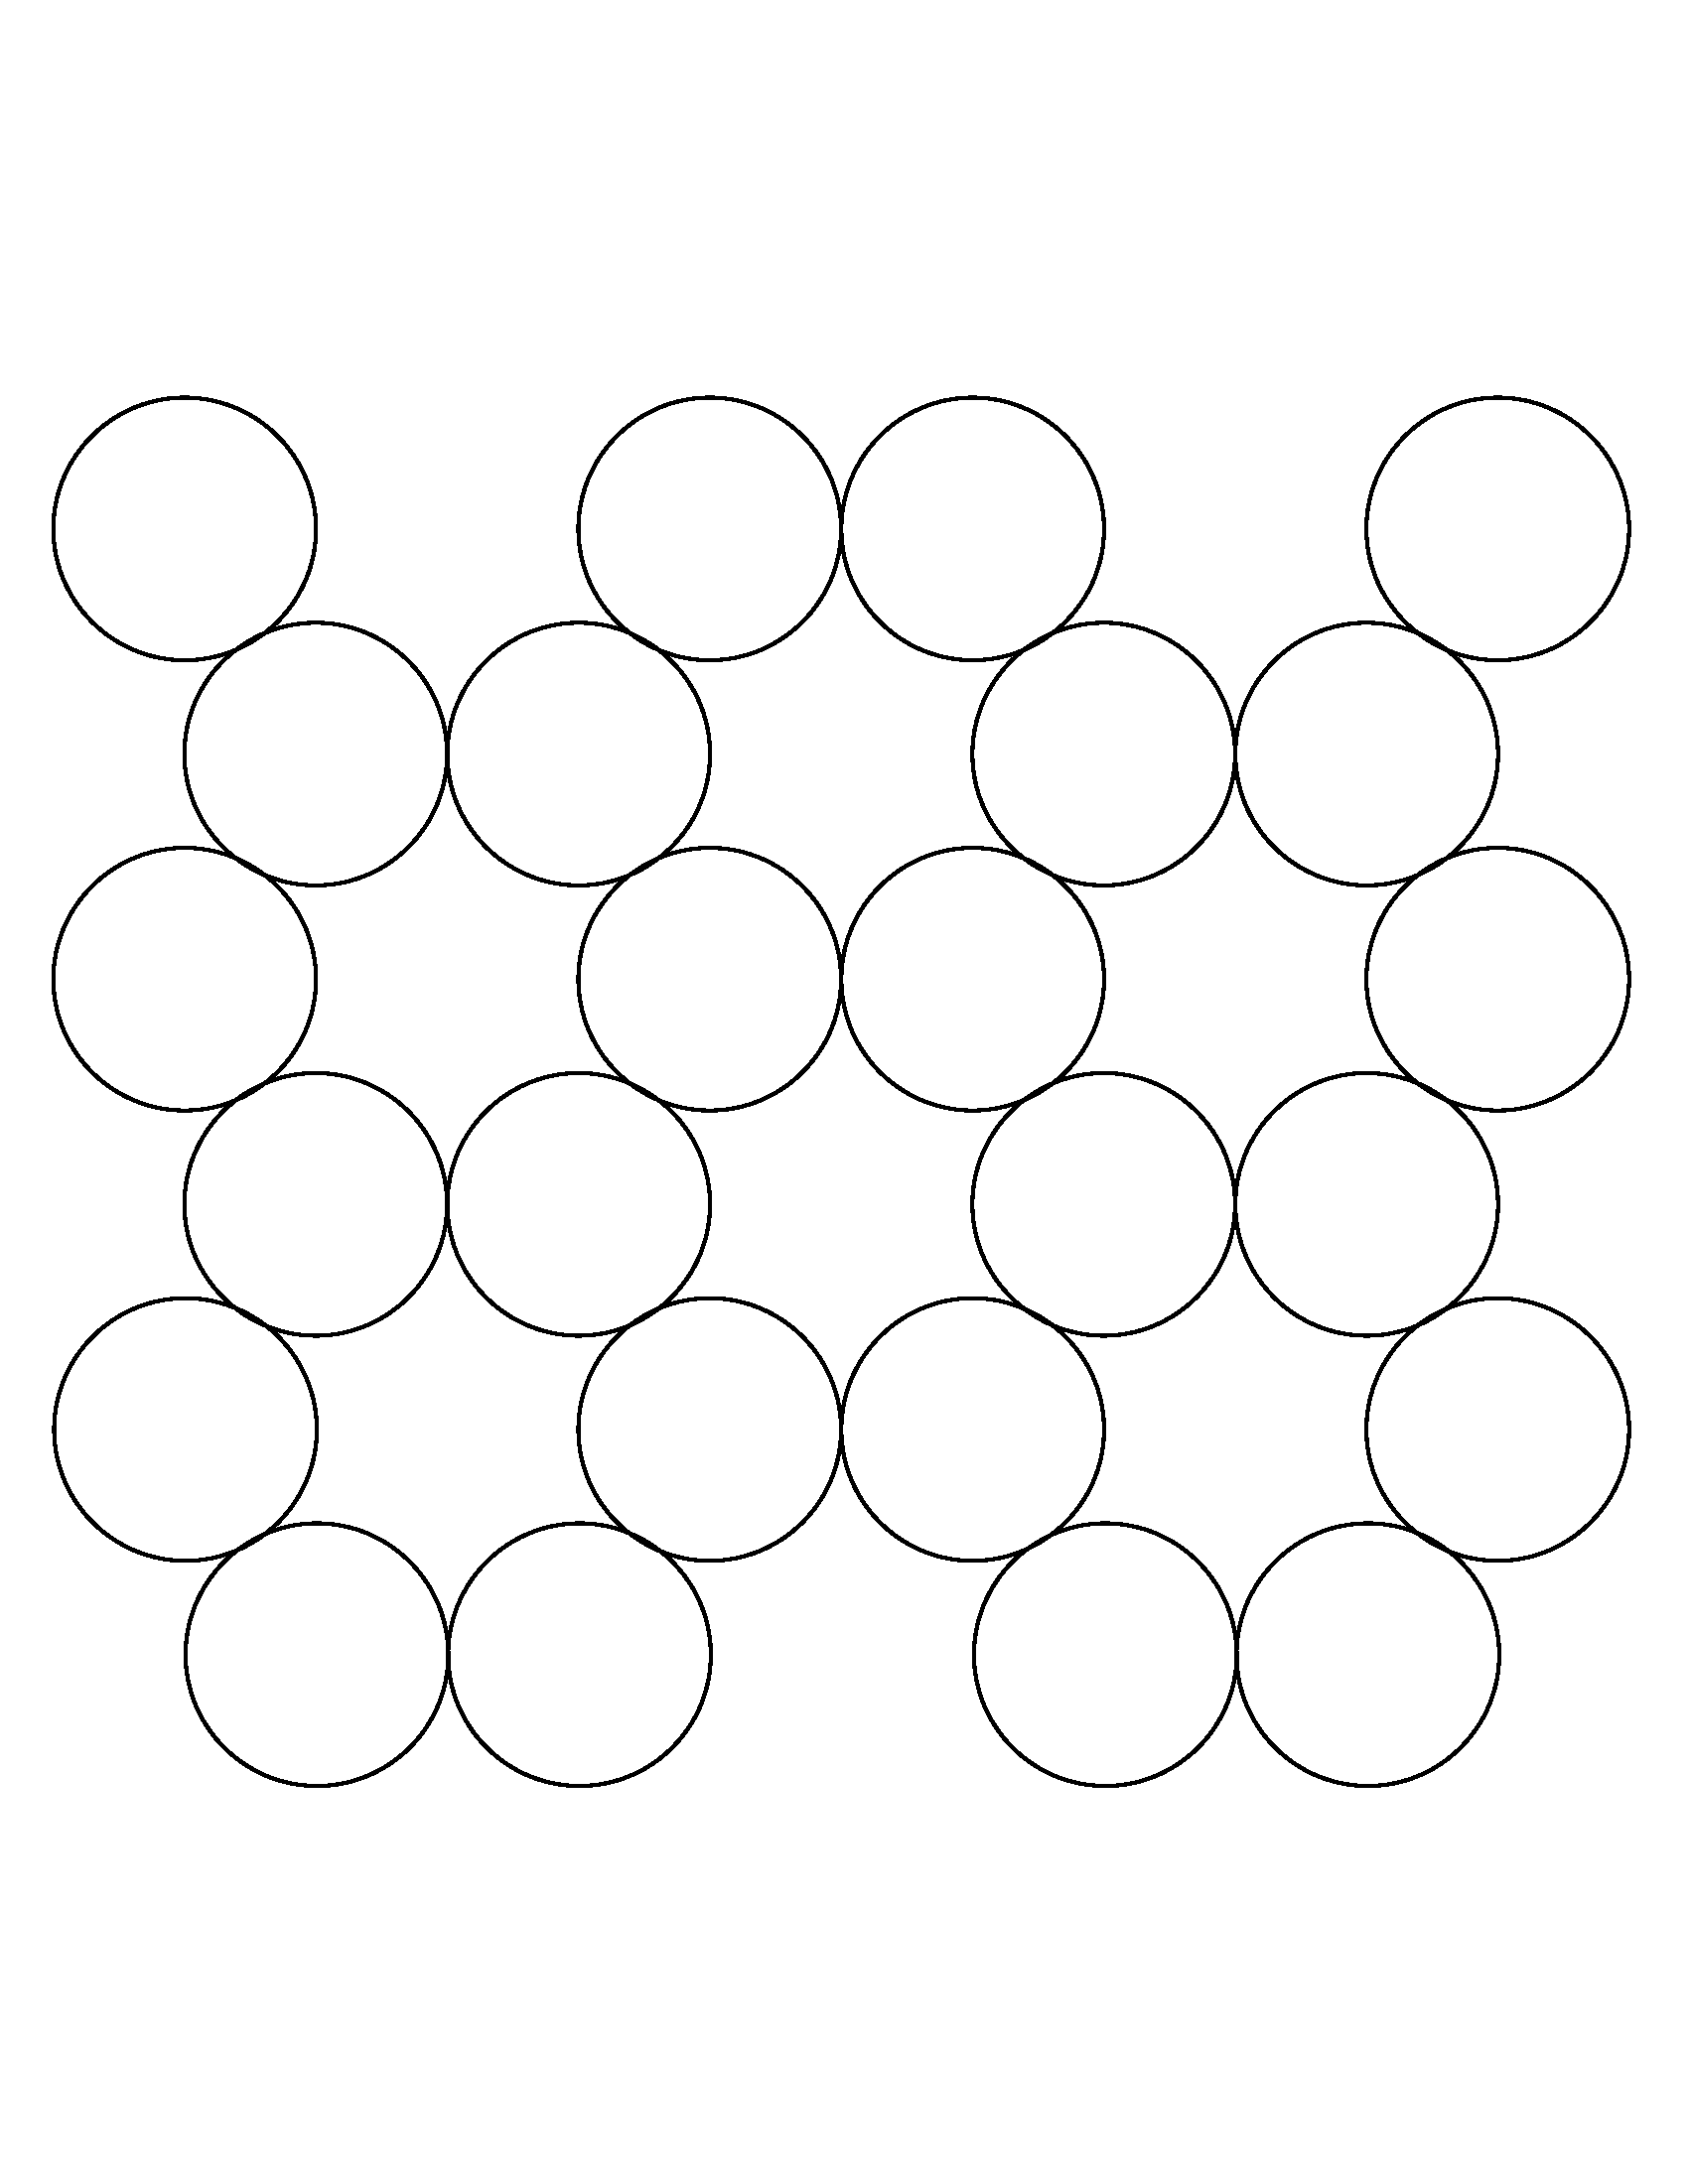
\includegraphics[width=2.7cm]{img/hex.png}
        \label{fig:ARCHalphas_11}
    }
    \subfigure[ SqueezeNext/SqNxt ]{
        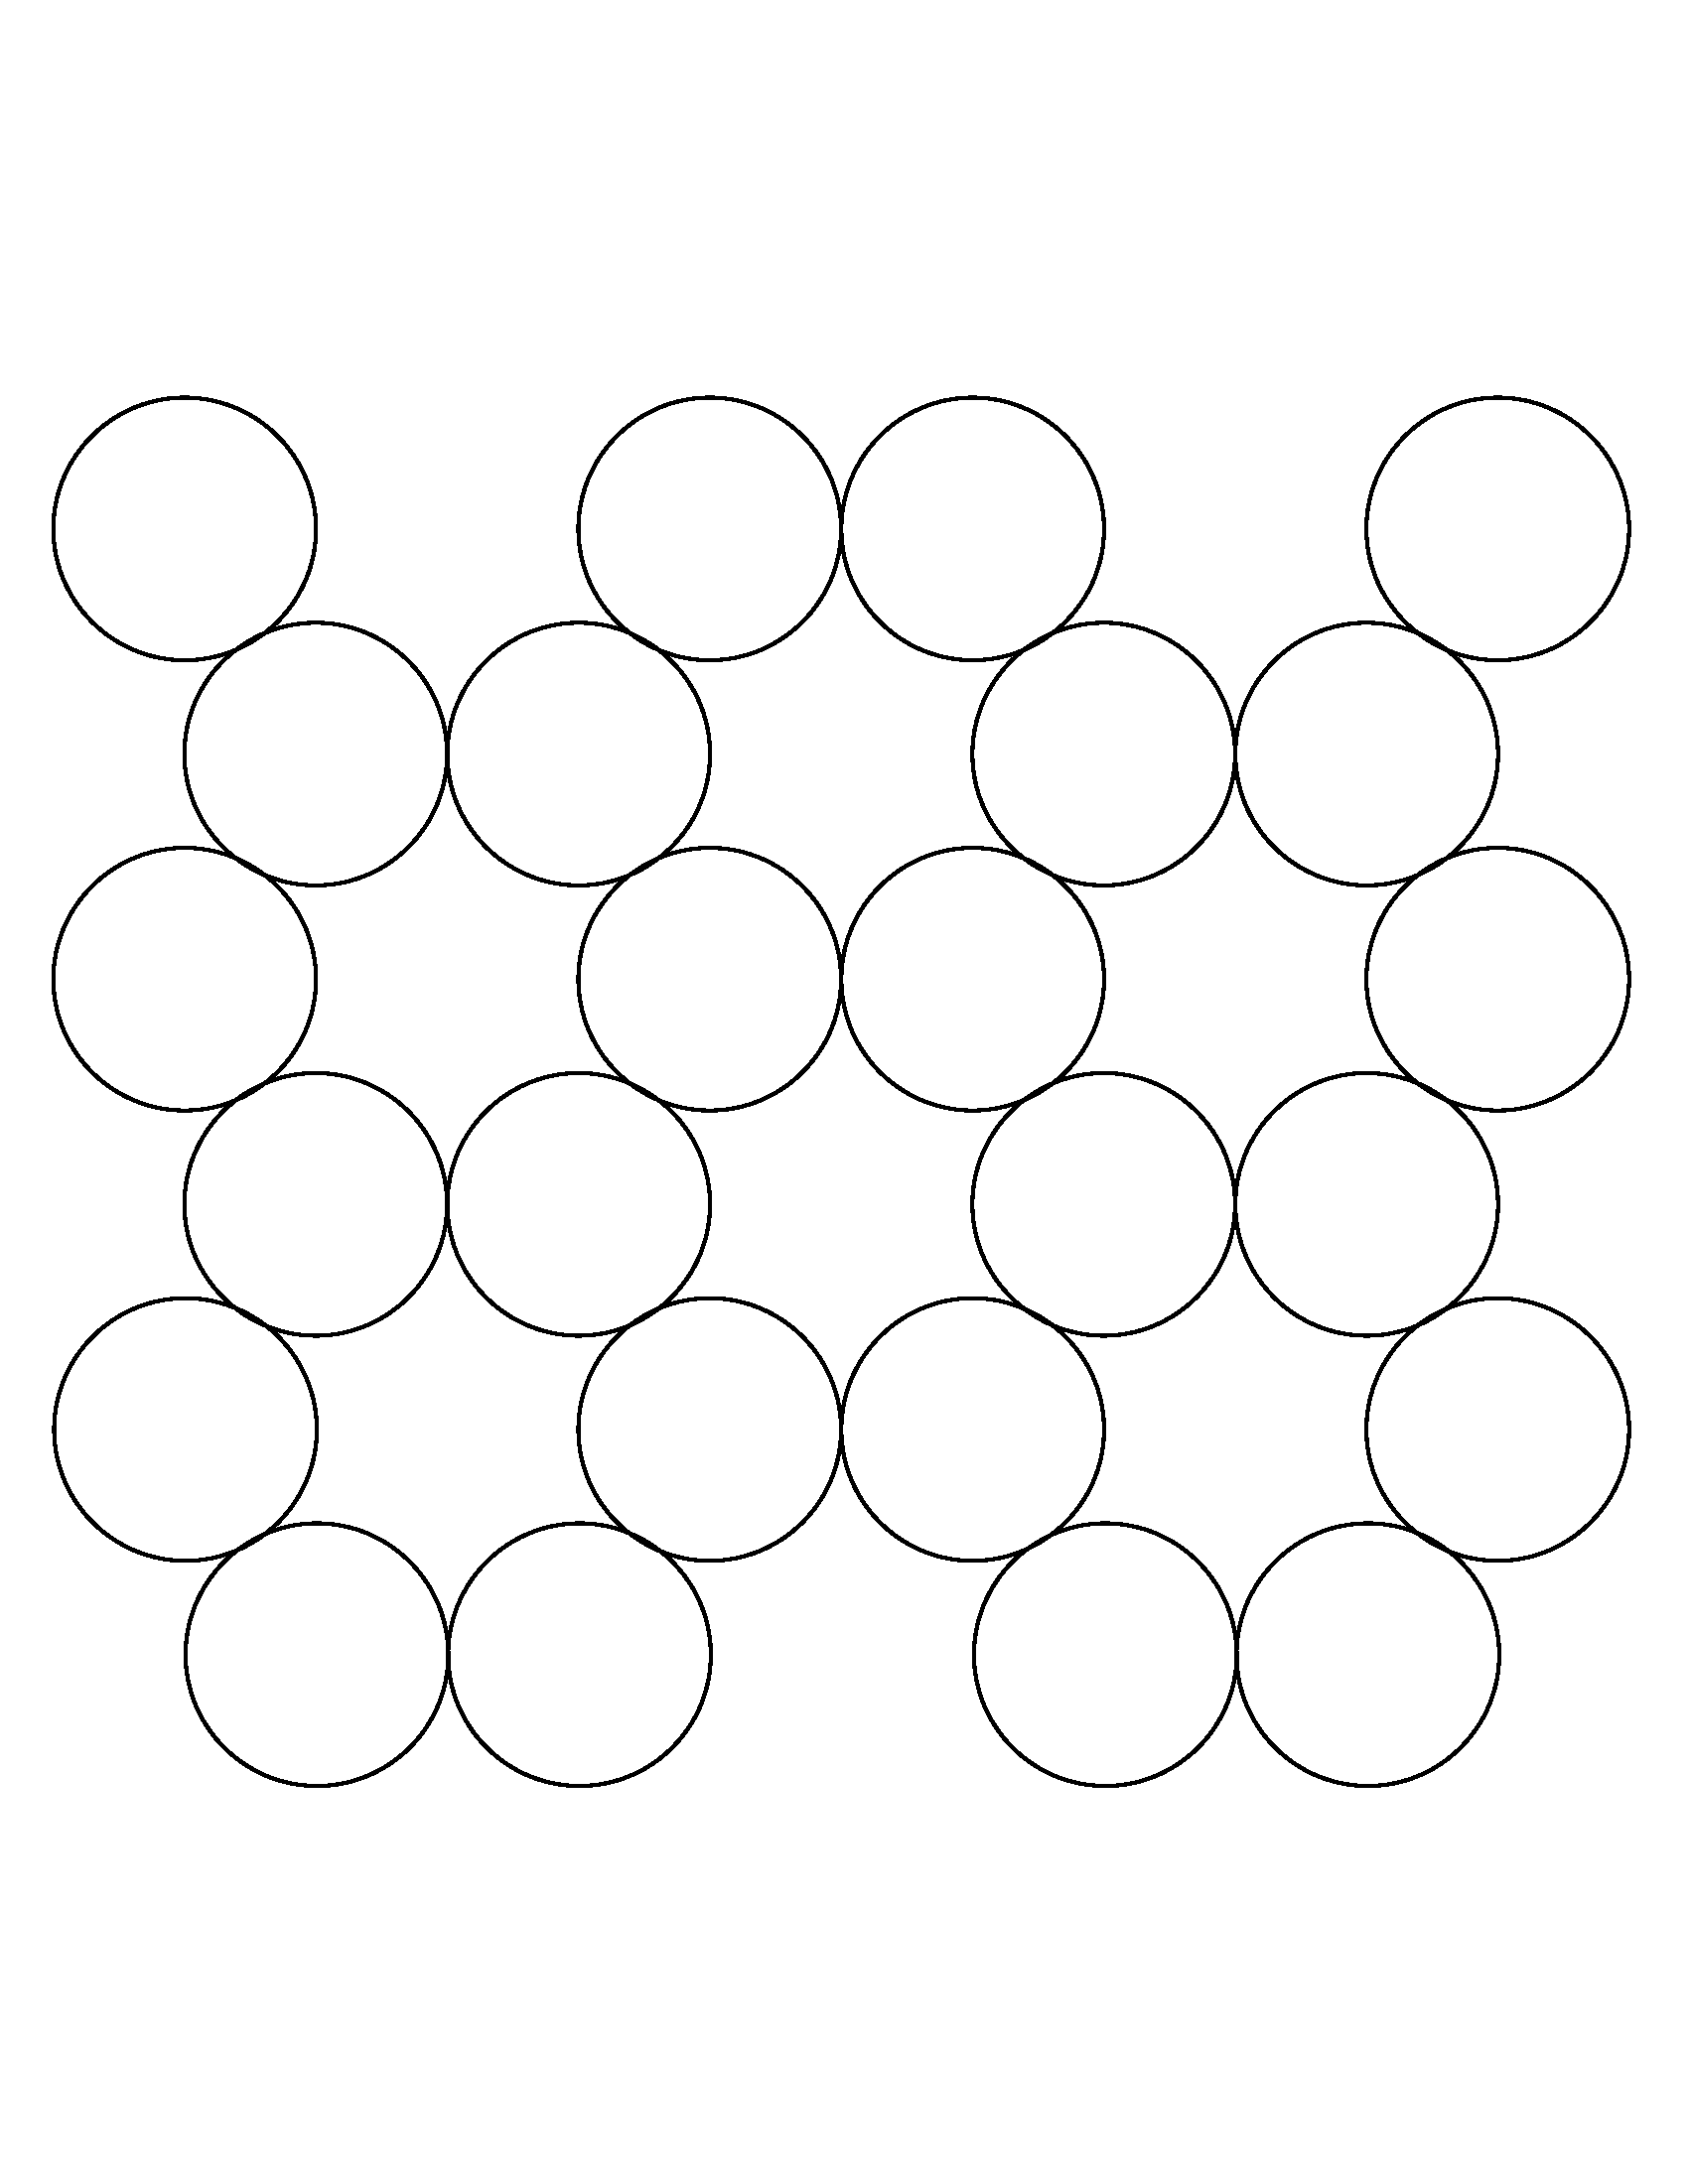
\includegraphics[width=2.7cm]{img/hex.png}
        \label{fig:ARCHalphas_12}
    }
    \subfigure[ ShuffleNet ]{
        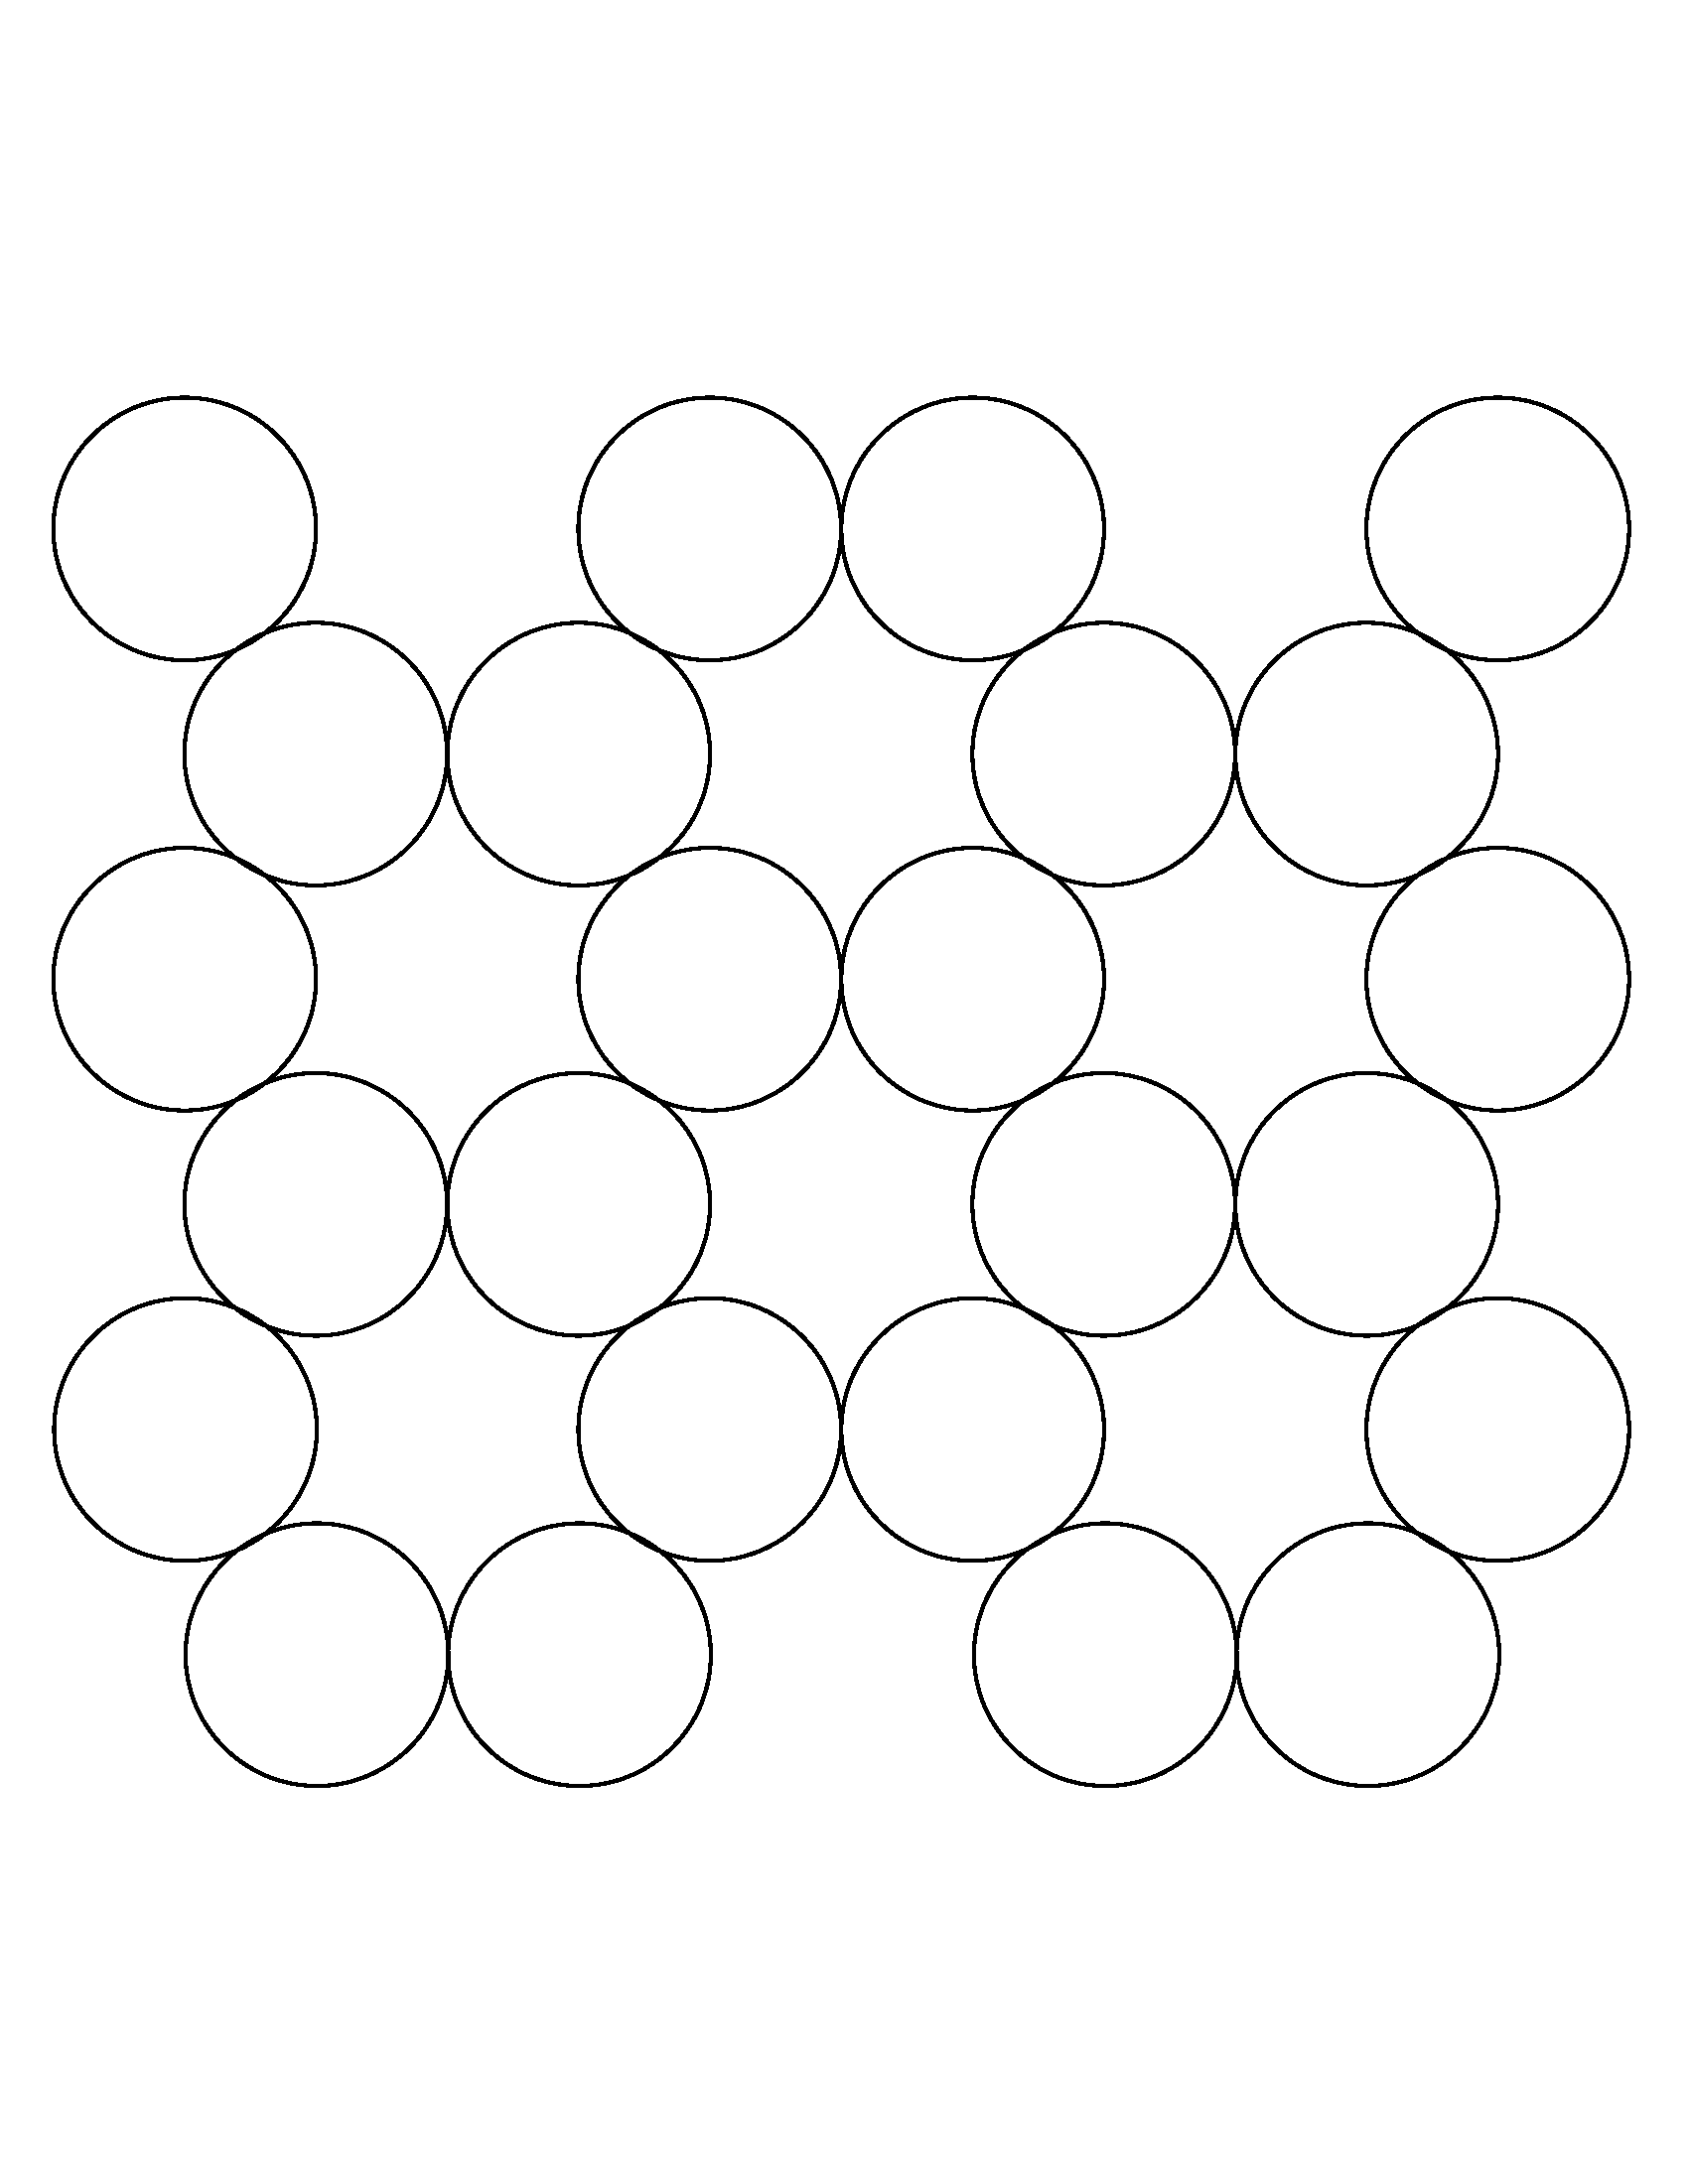
\includegraphics[width=2.7cm]{img/hex.png}
        \label{fig:ARCHalphas_13}
    }
    \subfigure[ DRN-C/DRN-D ]{
        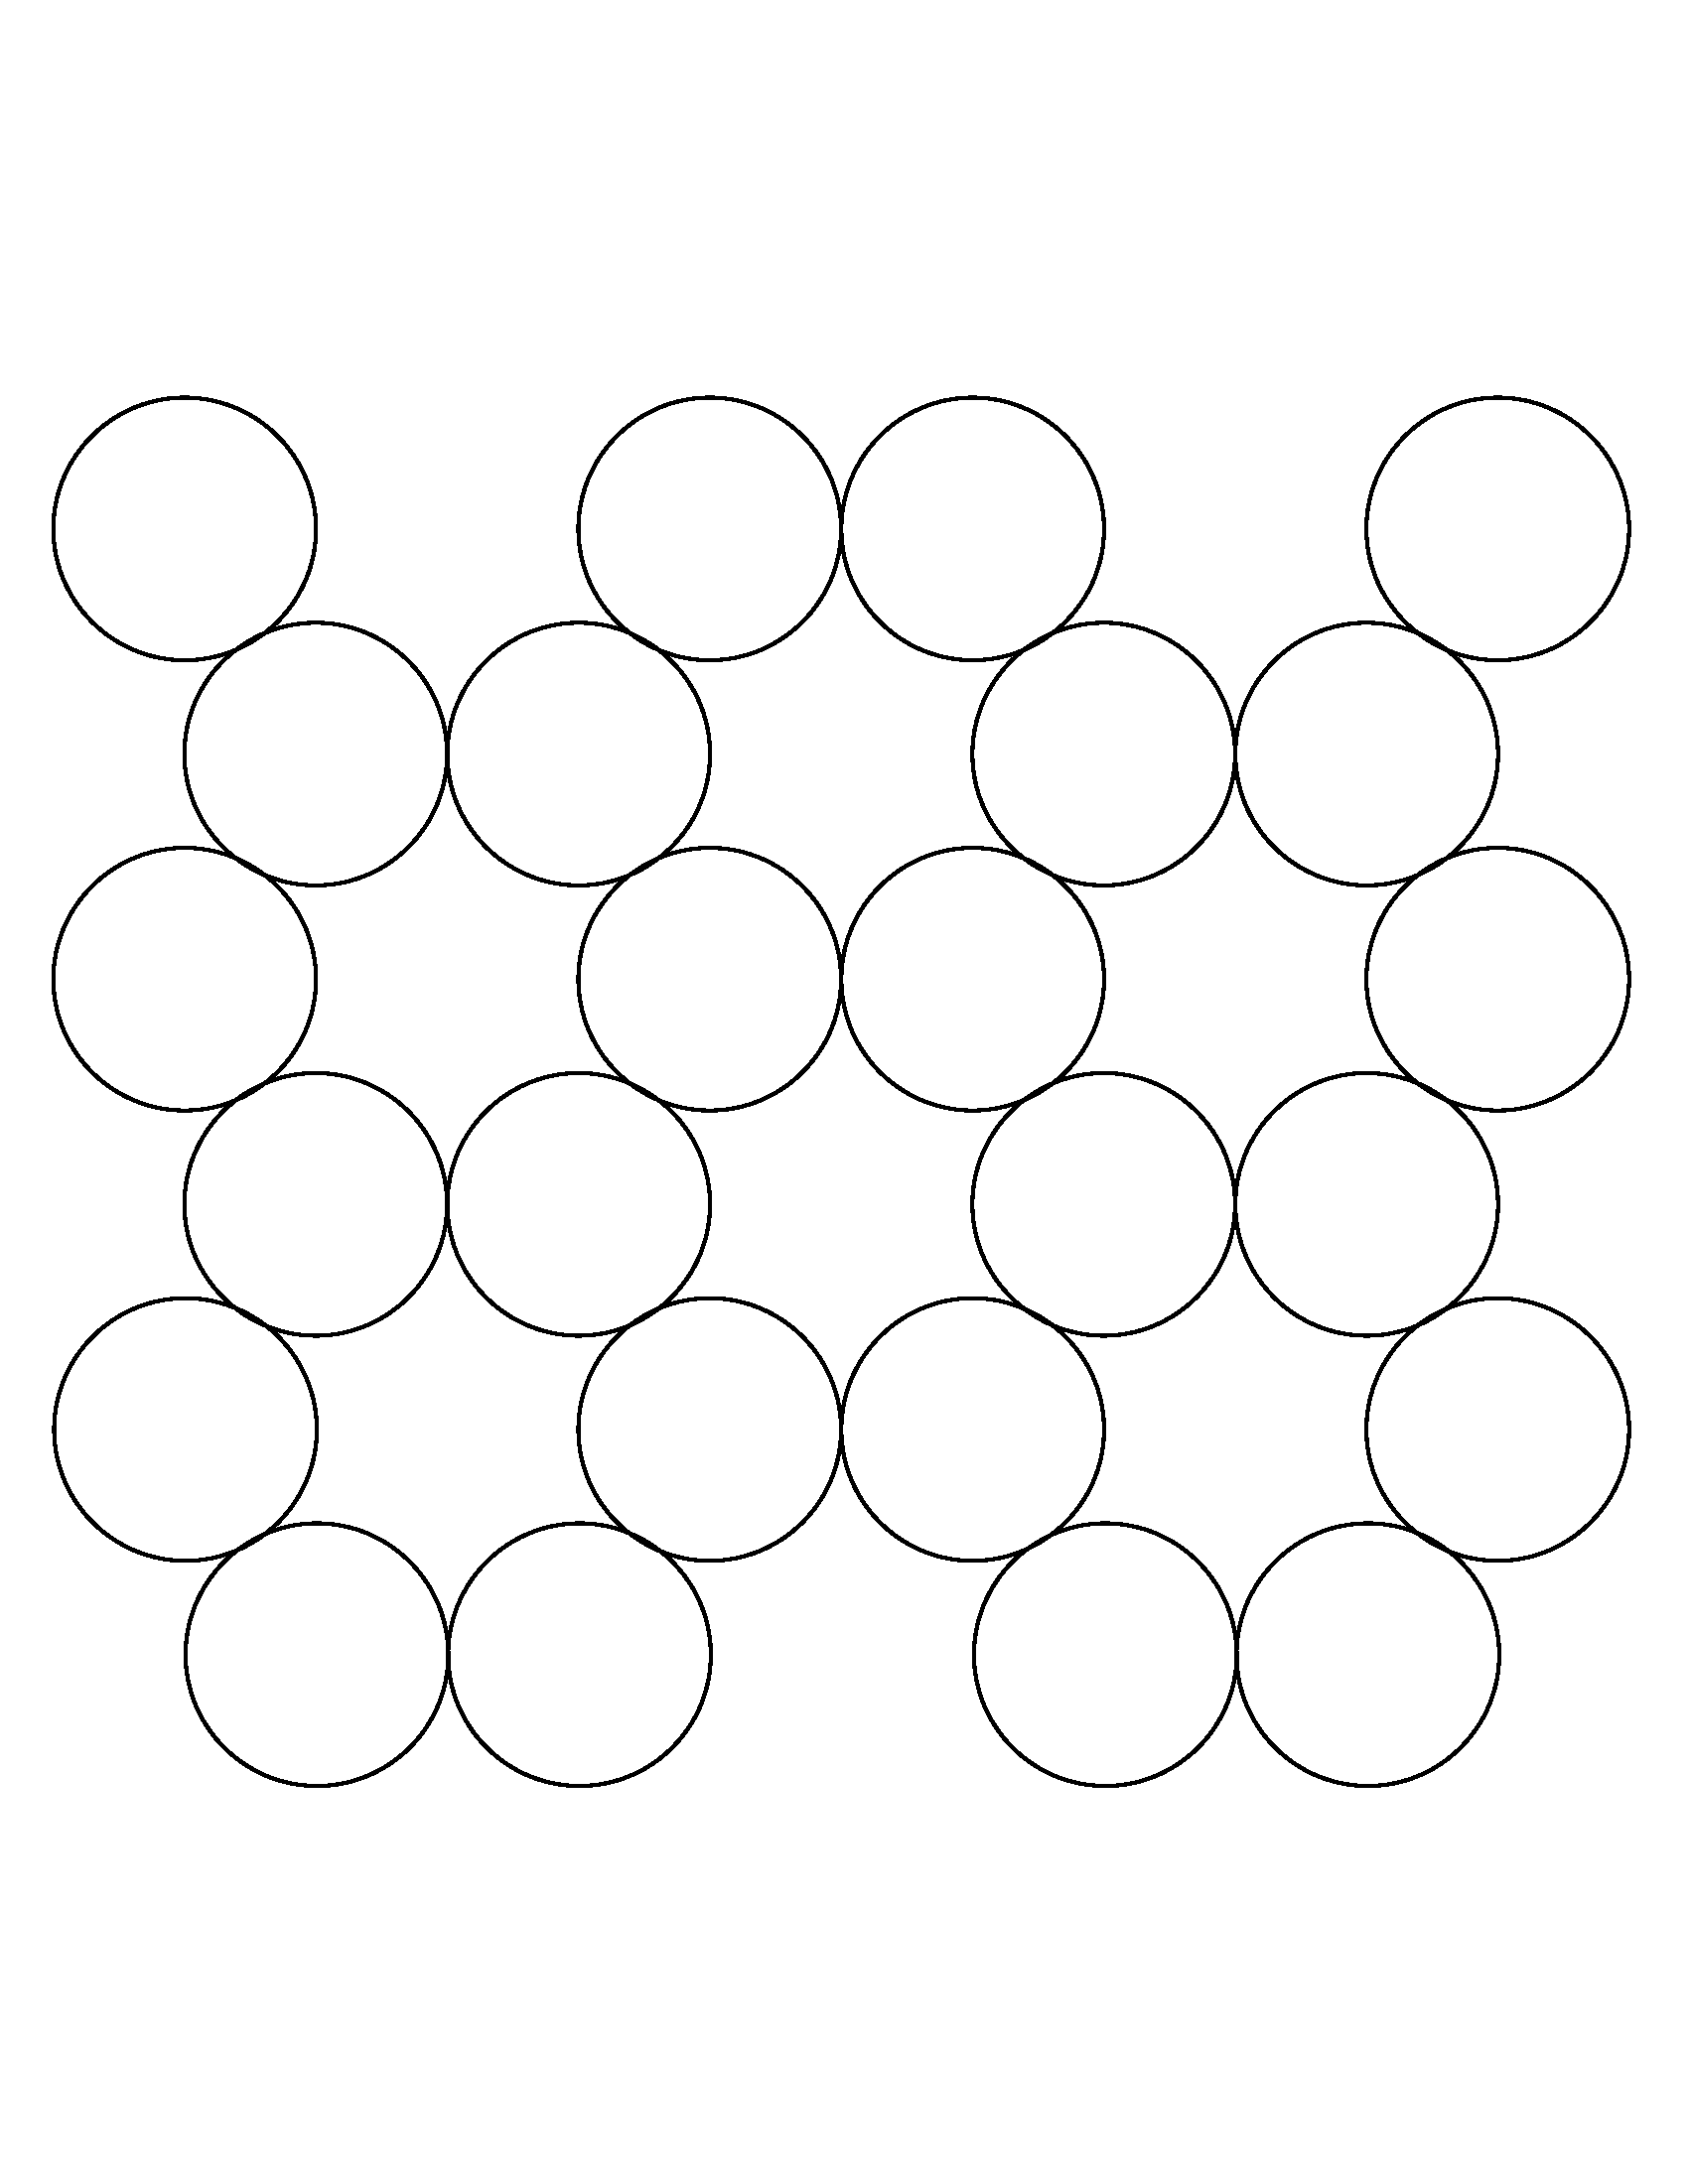
\includegraphics[width=2.7cm]{img/hex.png}
        \label{fig:ARCHalphas_14}
    }
    \subfigure[ ESPNetv2 ]{
        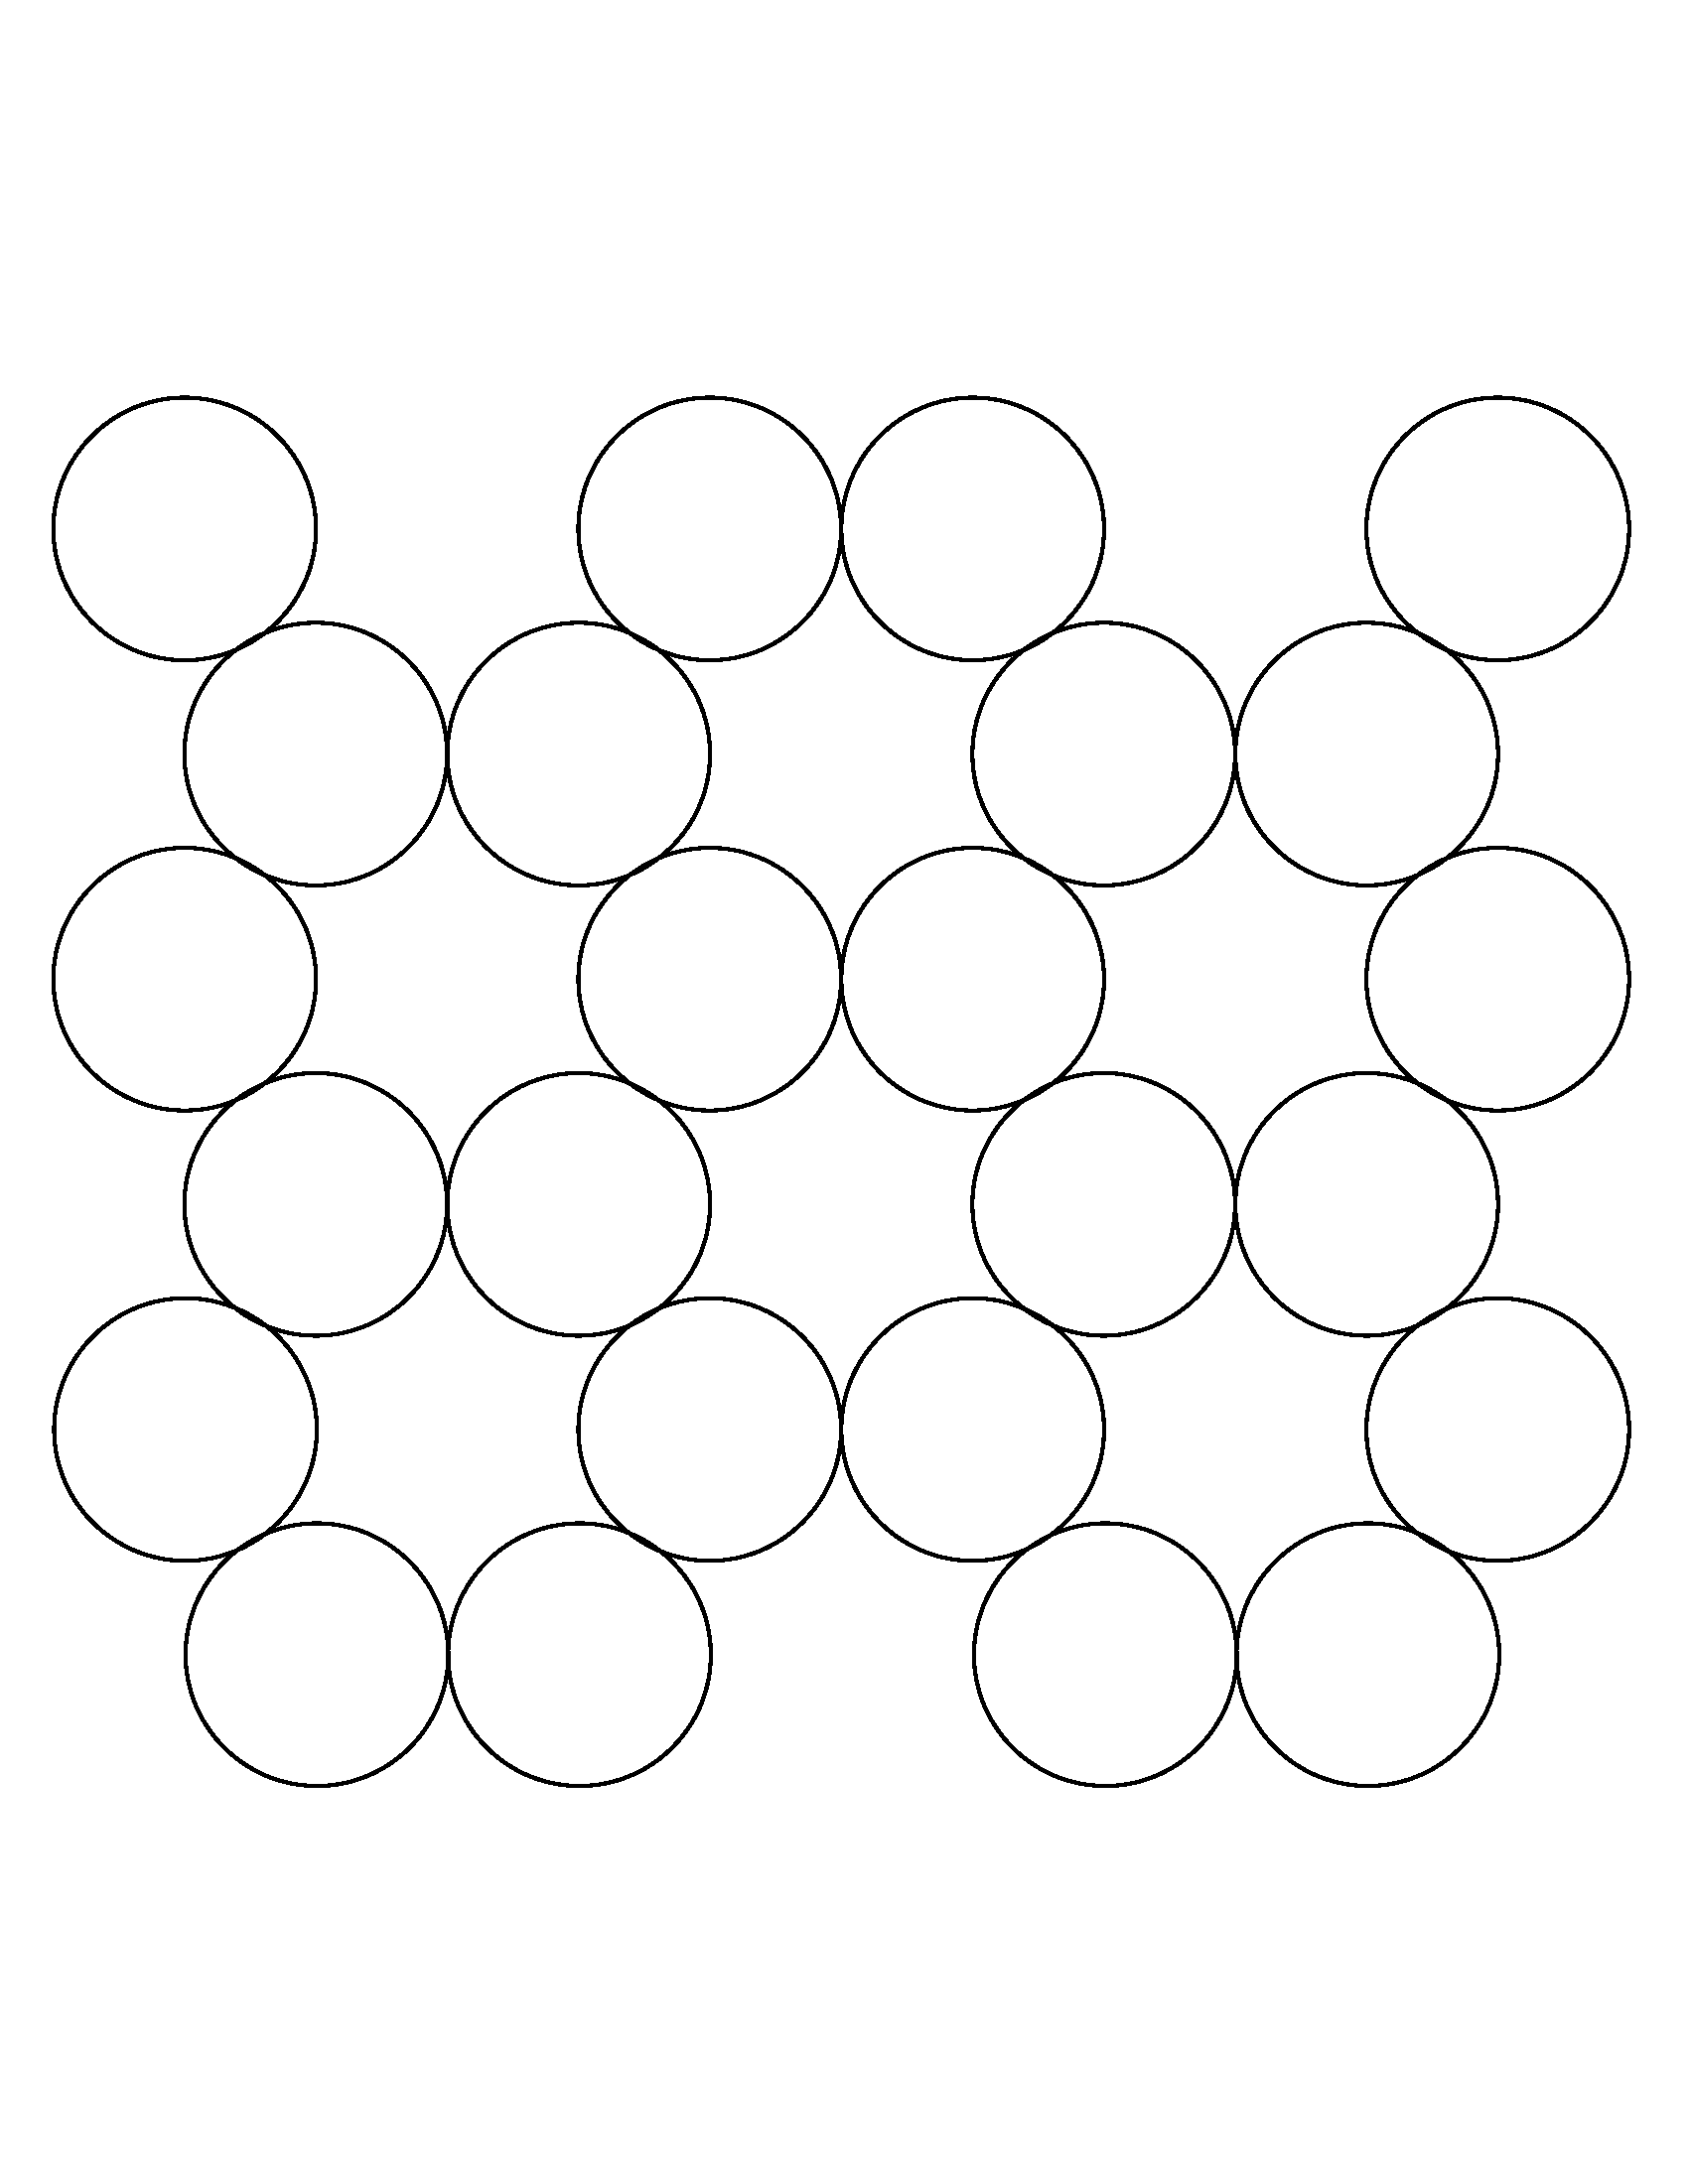
\includegraphics[width=2.7cm]{img/hex.png}
        \label{fig:ARCHalphas_15}
    }
    \subfigure[ HRNet ]{
        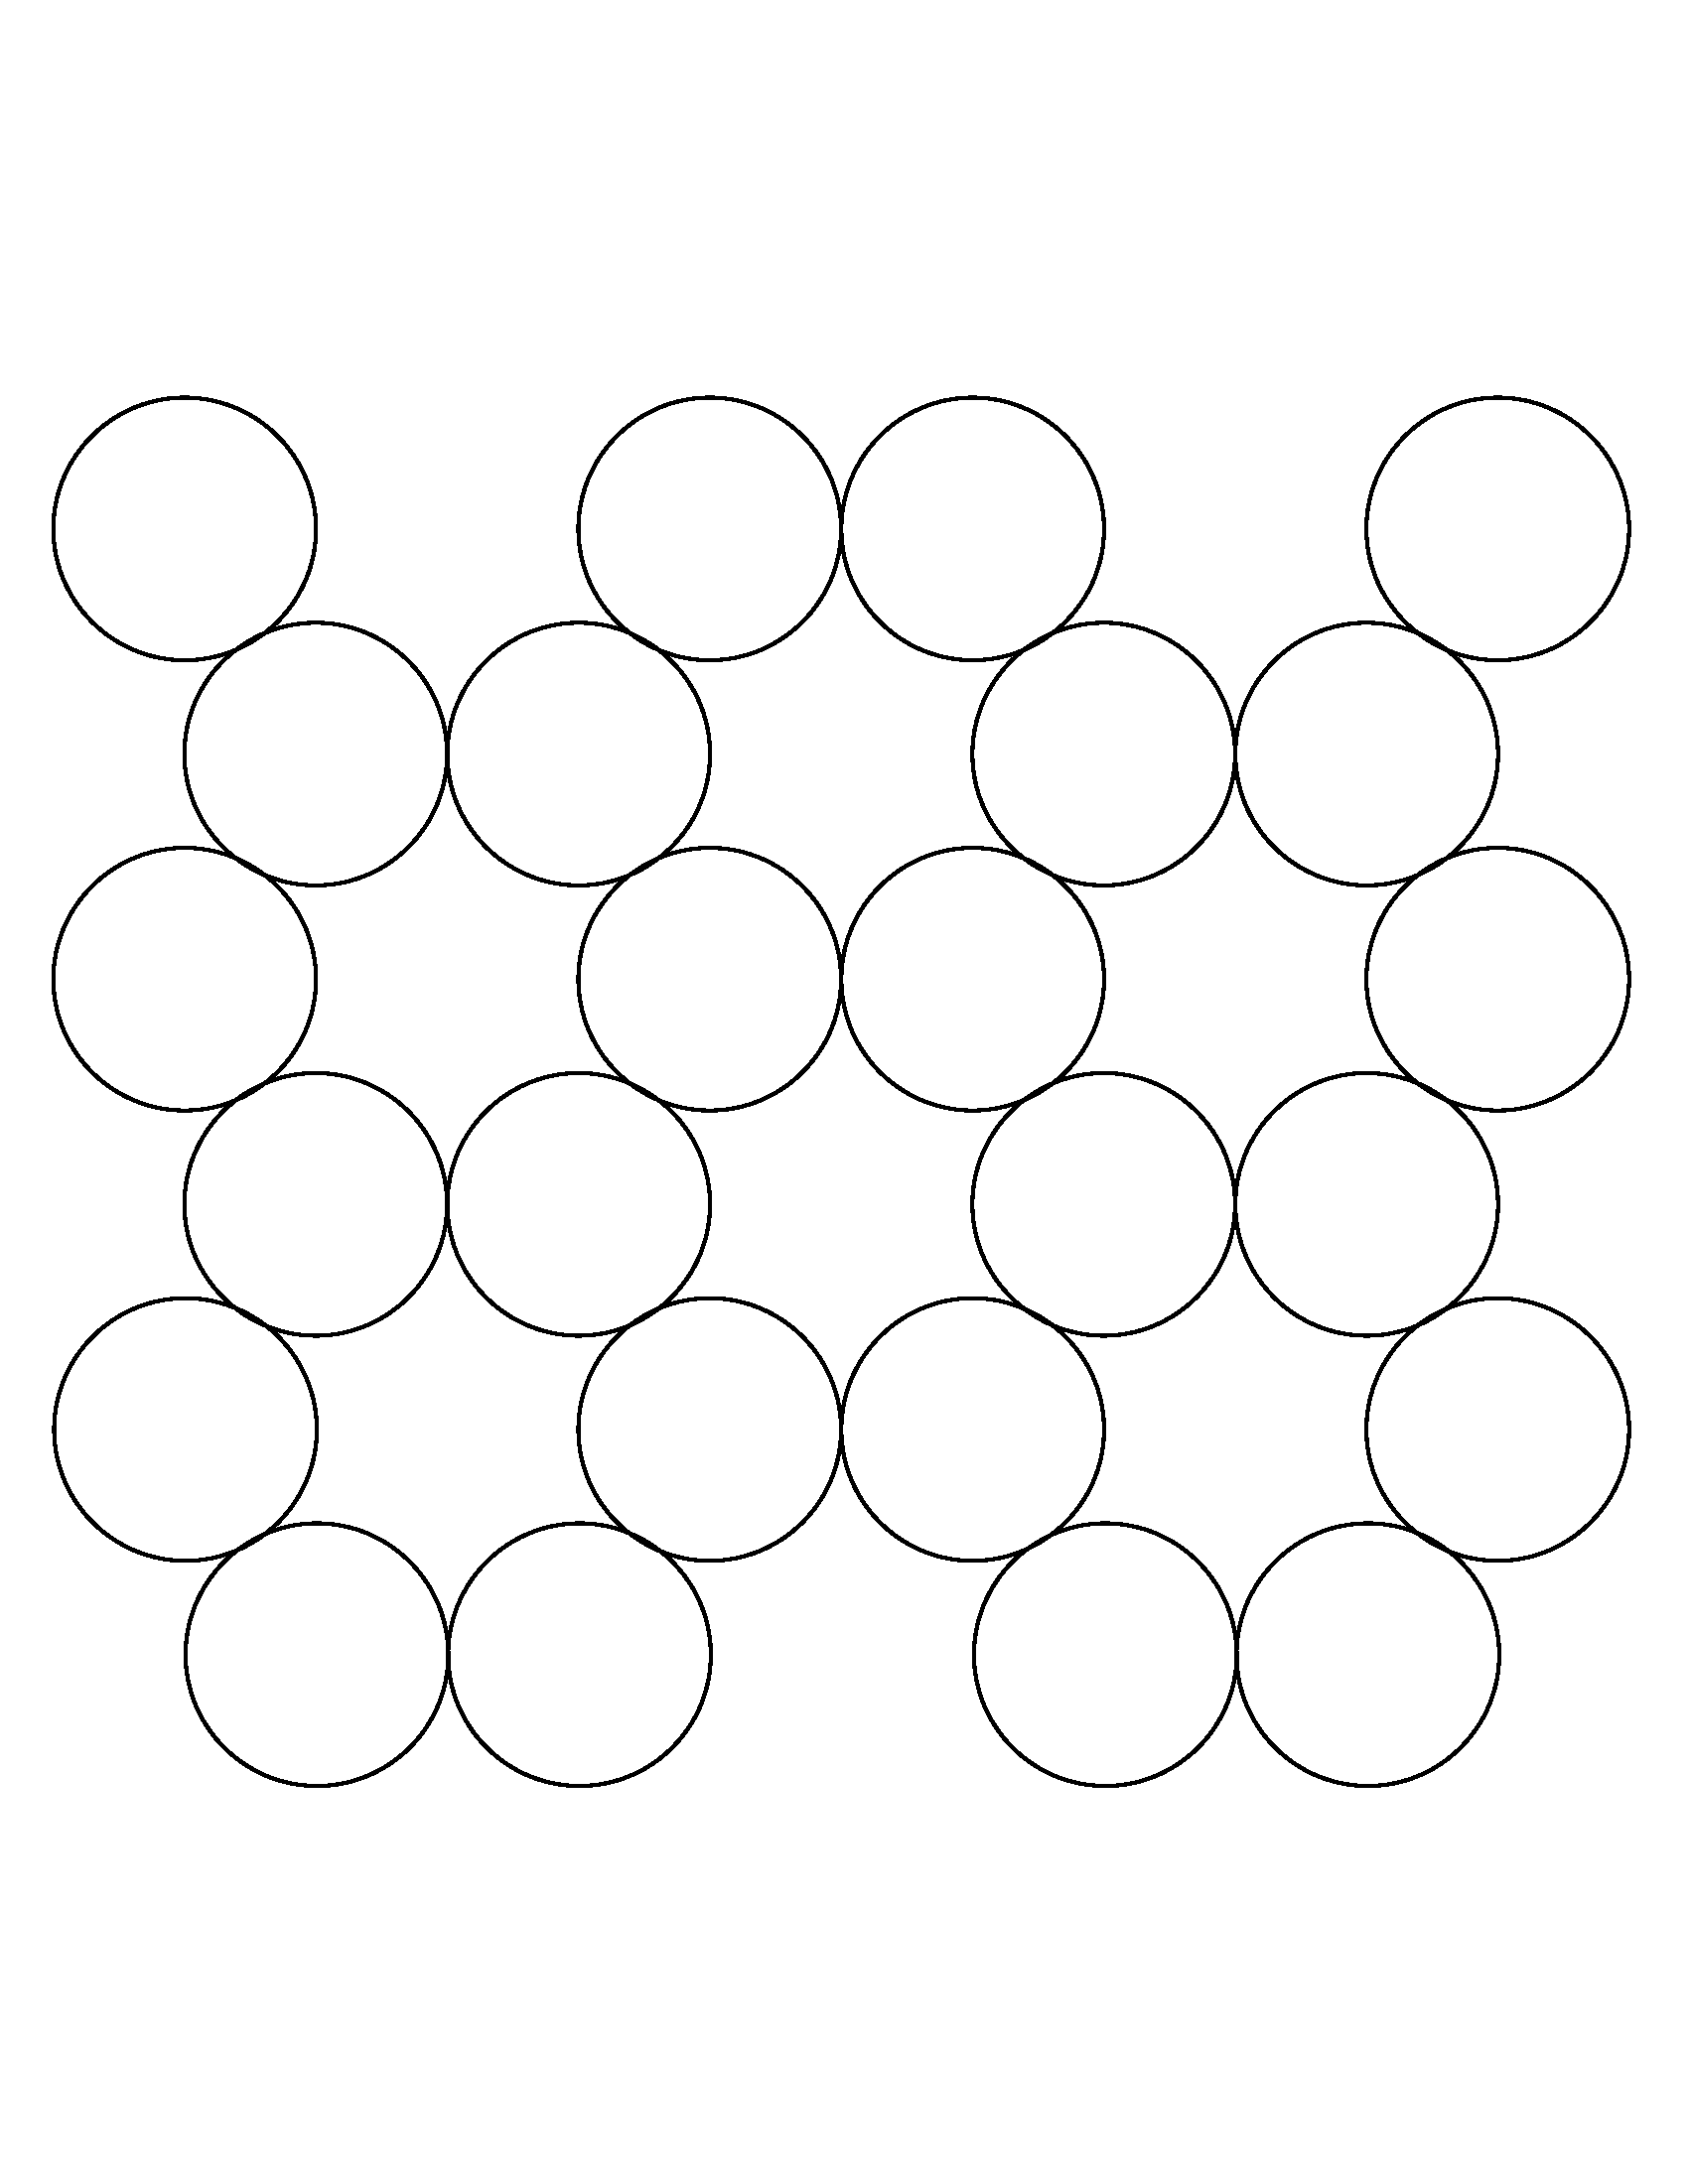
\includegraphics[width=2.7cm]{img/hex.png}
        \label{fig:ARCHalphas_16}
    }
    \subfigure[ SqueezeNet/SqueezeResNet ]{
        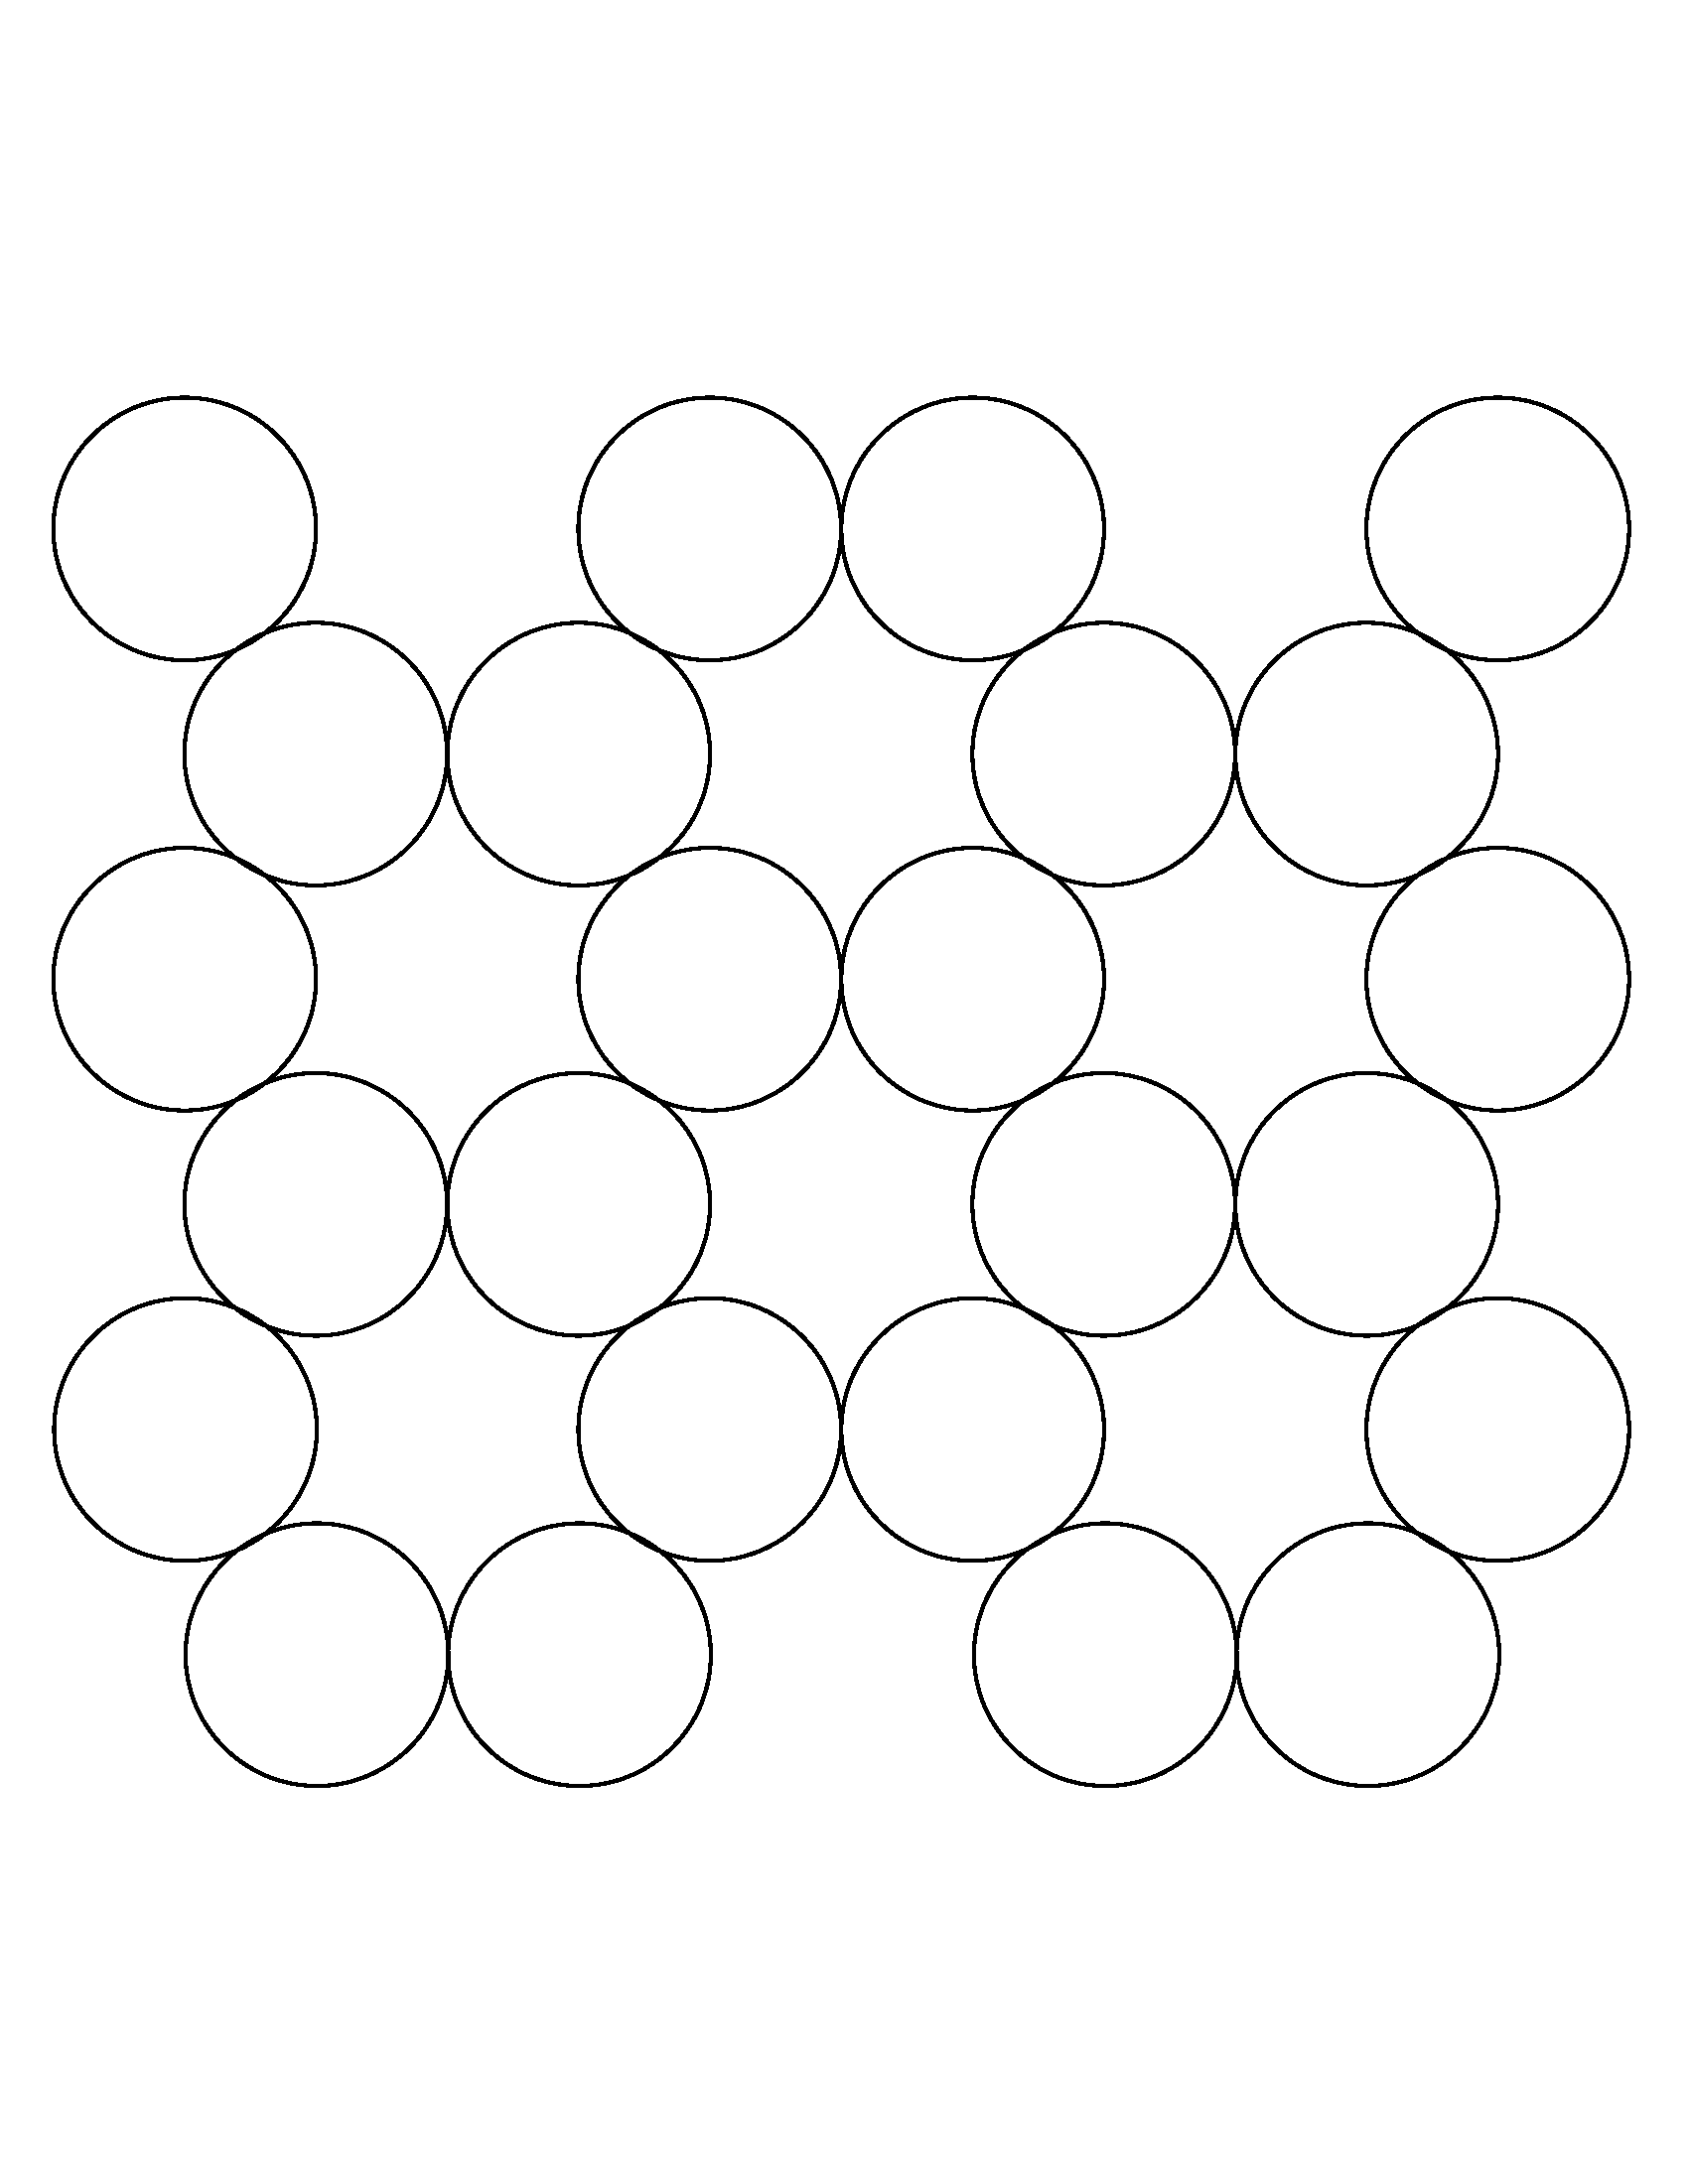
\includegraphics[width=2.7cm]{img/hex.png}
        \label{fig:ARCHalphas_17}
    }
    \caption{PL exponent $\alpha$ versus reported Top1 Test Accuracies for pretrained DNNs available for different architecture series (as segmented in Table~\ref{table:architectures}).
            }
    \label{fig:ARCHalphas}
\end{figure}

 
\begin{table}[t]
\scriptsize
\begin{center}
\begin{tabular}{|c|c|c|c|c|c|}
\hline
Dataset & Model  & $\langle\log\Vert\cdot\Vert_{F}\rangle$ & $\langle\log\Vert\cdot\Vert_{\infty}\rangle$ & $\hat{\alpha}$ & $\langle\log\Vert\cdot\Vert^{\alpha}_{\alpha}\rangle$ \\
\hline
 imagenet-1k & ResNet  & 5.96 &  11.03 & \textbf{3.51} & 4.01 \\
 imagenet-1k & EfficientNet  & 2.67 &  \textbf{1.23} & 2.56 & 2.50 \\
 imagenet-1k & PreResNet  & 6.59 &  15.44 & \textbf{3.59} & 3.71 \\
 imagenet-1k & ShuffleNet  & 35.38 &  89.58 & 19.54 & \textbf{18.48} \\
 imagenet-1k & VGG  & 0.84 &  \textbf{0.68} & 1.89 & 1.59 \\
 imagenet-1k & DLA  & 22.41 &  \textbf{8.49} & 14.69 & 15.68 \\
 imagenet-1k & HRNet  & 0.47 &  0.51 & \textbf{0.16} & 0.16 \\
 imagenet-1k & DRN-C  & 0.60 &  0.66 & \textbf{0.40} & 0.48 \\
 imagenet-1k & SqueezeNext  & 21.94 &  21.39 & 13.31 & \textbf{13.23} \\
 imagenet-1k & ESPNetv2  & 13.77 &  14.74 & \textbf{1.87} & 2.53 \\
 imagenet-1k & IGCV3  & 1.94 &  87.76 & 8.48 & \textbf{1.09} \\
 imagenet-1k & ProxylessNAS  & \textbf{0.19} &  0.26 & 0.28 & 0.26 \\
 imagenet-1k & SqueezeNet  & 0.11 &  0.11 & \textbf{0.07} & 0.08 \\
\hline
 cifar-10 & ResNet  & 0.31 &  0.30 & \textbf{0.28} & 0.28 \\
 cifar-10 & DIA-ResNet  & \textbf{0.05} &  0.08 & 0.28 & 0.32 \\
 cifar-10 & SENet  & 0.09 &  0.09 & \textbf{0.04} & 0.04 \\
\hline
 cifar-100 & ResNet  & 4.13 &  4.50 & \textbf{3.06} & 3.06 \\
 cifar-100 & DIA-ResNet  & \textbf{0.36} &  1.38 & 0.93 & 1.02 \\
 cifar-100 & SENet  & 0.36 &  0.43 & \textbf{0.26} & 0.26 \\
 cifar-100 & WRN  & 0.14 &  0.20 & 0.07 & \textbf{0.06} \\
\hline
 svhn & ResNet  & 0.04 &  0.04 & \textbf{0.02} & 0.02 \\
 svhn & DIA-ResNet  & 0.00 &  \textbf{0.00} & 0.02 & 0.02 \\
 svhn & SENet  & \textbf{0.00} &  0.00 & 0.00 & 0.00 \\
 svhn & WRN  & 0.01 &  0.01 & 0.01 & \textbf{0.01} \\
 svhn & ResNeXt  & 0.00 &  \textbf{0.00} & 0.01 & 0.01 \\
\hline
 cub-200-2011 & ResNet  & 0.20 &  \textbf{0.18} & 3.19 & 3.21 \\
 cub-200-2011 & SENet  & \textbf{1.07} &  1.29 & 1.85 & 1.95 \\
\hline
\end{tabular}
\end{center}
\vspace{-5mm}
\caption{$MSE$ results for our analysis of all CV models in Table~\ref{table:datasets}. }
\label{table:MSEresults}
\end{table}


\begin{table}[t]
\scriptsize
\begin{center}
\begin{tabular}{|c|c|c|c|c|c|}
\hline
Dataset & Model  & $\langle\log\Vert\cdot\Vert_{F}\rangle$ & $\langle\log\Vert\cdot\Vert_{\infty}\rangle$ & $\hat{\alpha}$ & $\langle\log\Vert\cdot\Vert^{\alpha}_{\alpha}\rangle$ \\
\hline
imagenet-1k & ResNet  & 0.82 &  0.67 & \textbf{0.90} & 0.88 \\
 imagenet-1k & EfficientNet  & 0.65 &  \textbf{0.84} & 0.67 & 0.67 \\
 imagenet-1k & PreResNet  & 0.73 &  0.36 & \textbf{0.85} & 0.85 \\
 imagenet-1k & ShuffleNet  & 0.63 &  0.06 & 0.80 & \textbf{0.81} \\
 imagenet-1k & VGG  & 0.71 &  \textbf{0.76} & 0.35 & 0.45 \\
 imagenet-1k & DLA  & 0.13 &  \textbf{0.67} & 0.43 & 0.39 \\
 imagenet-1k & HRNet  & 0.91 &  0.90 & \textbf{0.97} & 0.97 \\
 imagenet-1k & DRN-C  & 0.81 &  0.79 & \textbf{0.87} & 0.85 \\
 imagenet-1k & SqueezeNext  & 0.05 &  0.07 & 0.42 & \textbf{0.43} \\
 imagenet-1k & ESPNetv2  & 0.42 &  0.38 & \textbf{0.92} & 0.89 \\
 imagenet-1k & IGCV3  & 0.98 &  0.12 & 0.92 & \textbf{0.99} \\
 imagenet-1k & SqueezeNet  & 0.01 &  0.00 & \textbf{0.38} & 0.26 \\
 imagenet-1k & ProxylessNAS  & \textbf{0.68} &  0.56 & 0.53 & 0.58 \\
\hline
 cifar-10 & ResNet  & 0.58 &  0.59 & \textbf{0.62} & 0.61 \\
 cifar-10 & DIA-ResNet  & \textbf{0.96} &  0.93 & 0.74 & 0.71 \\
 cifar-10 & SENet  & 0.91 &  0.91 & \textbf{0.96} & 0.96 \\
\hline
 cifar-100 & ResNet  & 0.61 &  0.58 & \textbf{0.71} & 0.71 \\
 cifar-100 & DIA-ResNet  & \textbf{0.96} &  0.85 & 0.90 & 0.89 \\
 cifar-100 & SENet  & 0.97 &  0.96 & \textbf{0.98} & 0.98 \\
 cifar-100 & WRN  & 0.32 &  0.04 & 0.66 & \textbf{0.69} \\
\hline
 svhn & ResNet  & 0.69 &  0.70 & \textbf{0.82} & 0.81 \\
 svhn & DIA-ResNet  & 0.94 &  \textbf{0.95} & 0.78 & 0.77 \\
 svhn & SENet  & \textbf{0.99} &  0.96 & 0.98 & 0.98 \\
 svhn & WRN  & 0.13 &  0.10 & 0.20 & \textbf{0.21} \\
 svhn & ResNeXt  & 0.87 &  \textbf{0.90} & 0.64 & 0.75 \\
\hline
 cub-200-2011 & ResNet  & 0.94 &  \textbf{0.95} & 0.08 & 0.08 \\
 cub-200-2011 & SENet  & \textbf{0.66} &  0.59 & 0.41 & 0.38 \\
\hline
\end{tabular}
\end{center}
\vspace{-5mm}
\caption{$R^{2}$ results for our analysis of all CV models in Table~\ref{table:datasets}. }
\label{table:R2results}
\end{table}


\begin{table}[t]
\scriptsize
\begin{center}
\begin{tabular}{|c|c|c|c|c|c|}
\hline
Dataset & Model  & $\langle\log\Vert\cdot\Vert_{F}\rangle$ & $\langle\log\Vert\cdot\Vert_{\infty}\rangle$ & $\hat{\alpha}$ & $\langle\log\Vert\cdot\Vert^{\alpha}_{\alpha}\rangle$ \\
\hline
 imagenet-1k  & ResNet        &  XXX &   XXX &  XXX &  XXX \\
 imagenet-1k  & EfficientNet  &  XXX &   XXX &  XXX &  XXX \\
 imagenet-1k  & PreResNet     &  XXX &   XXX &  XXX &  XXX \\
 imagenet-1k  & ShuffleNet    &  XXX &   XXX &  XXX &  XXX \\
 imagenet-1k  & VGG           &  XXX &   XXX &  XXX &  XXX \\
 imagenet-1k  & DLA           &  XXX &   XXX &  XXX &  XXX \\
 imagenet-1k  & HRNet         &  XXX &   XXX &  XXX &  XXX \\
 imagenet-1k  & DRN-C         &  XXX &   XXX &  XXX &  XXX \\
 imagenet-1k  & SqueezeNext   &  XXX &   XXX &  XXX &  XXX \\
 imagenet-1k  & ESPNetv2      &  XXX &   XXX &  XXX &  XXX \\
 imagenet-1k  & IGCV3         &  XXX &   XXX &  XXX &  XXX \\
 imagenet-1k  & SqueezeNet    &  XXX &   XXX &  XXX &  XXX \\
 imagenet-1k  & ProxylessNAS  &  XXX &   XXX &  XXX &  XXX \\
\hline
 cifar-10     & ResNet        &  XXX &   XXX &  XXX &  XXX \\
 cifar-10     & DIA-ResNet    &  XXX &   XXX &  XXX &  XXX \\
 cifar-10     & SENet         &  XXX &   XXX &  XXX &  XXX \\
\hline
 cifar-100    & ResNet        &  XXX &   XXX &  XXX &  XXX \\
 cifar-100    & DIA-ResNet    &  XXX &   XXX &  XXX &  XXX \\
 cifar-100    & SENet         &  XXX &   XXX &  XXX &  XXX \\
 cifar-100    & WRN           &  XXX &   XXX &  XXX &  XXX \\
\hline
 svhn         & ResNet        &  XXX &   XXX &  XXX &  XXX \\
 svhn         & DIA-ResNet    &  XXX &   XXX &  XXX &  XXX \\
 svhn         & SENet         &  XXX &   XXX &  XXX &  XXX \\
 svhn         & WRN           &  XXX &   XXX &  XXX &  XXX \\
 svhn         & ResNeXt       &  XXX &   XXX &  XXX &  XXX \\
\hline
 cub-200-2011 & ResNet        &  XXX &   XXX &  XXX &  XXX \\
 cub-200-2011 & SENet         &  XXX &   XXX &  XXX &  XXX \\
\hline
\end{tabular}
\end{center}
\vspace{-5mm}
\caption{Kendall-$\tau$ results for our analysis of all CV models in Table~\ref{table:datasets}. }
\label{table:KTresults}
\end{table}


\subsection{Supplementary Figures}

\michael{The text in this section needs to be changed---probably not removed, but instead discuss things, not point to the figure we remove, and point to the repo. }

\michael{Do we get more visually compelling results if we present figures, but segmented by architectures, as listed in Table~\ref{table:architectures}; if so, perhaps we should put those, so we don't tell R1 that we just removed what looked bad; or maybe actually both, since we segment by dataset in Table~\ref{table:datasets}. }

To explain further how to reproduce our analysis, we run three batches of linear regressions. 
First, at the global level, we divide models by datasets and run regressions separately on all models of a certain dataset, regardless of the architecture. 
At this level, the plots are quite noisy and clustered, as each architecture has its own accuracy trend; but one can
 still see that most plots show positive relationship with positive coefficients. 
% V1 REMOVED FOR V2 % Example regressions are shown in Figure~\ref{fig:DSalphas}, as available in the results notebook.
Example regressions are shown in 
Figure~\ref{fig:DSalphas}, for models segmented by dataset, as listed in Table~\ref{table:datasets}, 
and in 
Figure~\ref{fig:ARCHalphas}, for models segmented by architecture, as listed in Table~\ref{table:architectures}.
\michael{Comment here on differences.}

To generate the results in Table~\ref{table:results}, we run linear regressions for each architecture series in Table~\ref{table:architectures}, regressing each empirical Log Norm metric against the reported Top1 (and Top5) errors (as listed on the \texttt{osmr/imgclsmob} github repository README file~\cite{osmr}, with the relevant data extracted and provided in our github repo as \texttt{pytorchcv.html}).
We record the $R^{2}$ and $MSE$ for each metric, averaged over all regressions for all architectures and datasets.
See Table~\ref{table:MSEresults}, Table~\ref{table:R2results}, and Table~\ref{table:KTresults}.
In the repo, plots are provided for every regression, and more fine grained results may be computed by the reader by analyzing the data in the \texttt{df\_all.xlsx} file.
The final analysis includes 108 regressions in all, those with 4 or more models, with a positive $R^2$.


\subsection{Supplementary Discussion: Additional Details on HT-SR Theory}

The original work on HT-SR Theory~\cite{MM18_TR,MM19_HTSR_ICML,MM20_SDM} considered NNs including AlexNet and InceptionV3 (as well as DenseNet, ResNet, and VGG), and it showed that for nearly every $\mathbf{W}$, the (bulk and tail) of the ESDs can be fit to a truncated PL and the PL exponents $\alpha$ nearly all lie within the range $\alpha\in(1.5,5)$.
Our meta-analysis, the main results of which are summarized in this paper, has shown that these results are ubiquitous.
For example, 
upon examining nearly 10,000 layer weight matrices $\mathbf{W}_{l,i}$ across hundreds of different modern pre-trained DNN architectures, the ESD of nearly every $\mathbf{W}$ layer matrix can be fit to a truncated PL:
$70-80\%$ of the time, the fitted PL exponent $\alpha$ lies in the range $\alpha\in(2,4)$; and  
$10-20\%$ of the time, the fitted PL exponent $\alpha$ lies in the range $\alpha< 2$.  
Of course, there are exceptions: in any real DNN, the fitted $\alpha$ may range anywhere from $\sim 1.5$ to $10$ or higher (and, of course, larger values of $\alpha$ may indicate that the PL is not a good model for the data).  
Still, overall, in nearly all large, pre-trained DNNs, the correlations in the  weight matrices exhibit a remarkable Universality, being both Heavy Tailed, and having small---but not too small---PL exponents. 


